\documentclass[12pt]{article}
\usepackage[letterpaper,margin=0.75in,headheight=14.5pt,headsep=0.22in,footskip=0.35in]{geometry}
\usepackage[T5,T1]{fontenc}
\usepackage[utf8]{inputenc}
\usepackage{lmodern}
\usepackage{amssymb}
\usepackage{array}
\usepackage{enumitem}
\usepackage{environ}
\usepackage{fancyhdr}
\usepackage{graphicx}
\usepackage{longtable}
\usepackage{needspace}
\usepackage{setspace}
\usepackage{tabularx}
\usepackage{titlesec}
\usepackage{xcolor}
\usepackage{float}
\usepackage{booktabs}
\usepackage{hyperref}
\usepackage{mdframed}

\definecolor{HCMUSBlue}{RGB}{0,112,192}
\setlength{\parindent}{0pt}
\setlength{\parskip}{0pt}
\setstretch{1.5}
\setcounter{secnumdepth}{2}
\setcounter{tocdepth}{2}

\titleformat{\section}
  {\color{HCMUSBlue}\bfseries\fontsize{22}{27}\selectfont}
  {\thesection}{0.5em}{}
\titleformat{\subsection}
  {\bfseries\fontsize{16}{20}\selectfont}
  {\thesubsection}{0.6em}{}
\titlespacing*{\section}{0pt}{12pt}{6pt}
\titlespacing*{\subsection}{0pt}{10pt}{4pt}

\newcolumntype{L}{>{\raggedright\arraybackslash}X}
\newcolumntype{C}{>{\centering\arraybackslash}X}
\newcommand{\blankcell}{\rule{0pt}{2.6ex}}
\newcommand{\vnname}[1]{{\fontencoding{T5}\selectfont #1}}
\NewEnviron{srstable}[1]{%
  \begin{center}\small
  \renewcommand{\arraystretch}{1.2}
  \setlength{\tabcolsep}{4pt}
  \begin{tabularx}{\textwidth}{|#1|}\hline
  \BODY
  \end{tabularx}\end{center}
}

\newenvironment{usecasebox}[1]{%
  \begin{mdframed}[frametitle={#1},frametitlebackgroundcolor=HCMUSBlue,frametitlefont=\color{white}\bfseries,linecolor=HCMUSBlue,linewidth=0.7pt,roundcorner=0pt,innerleftmargin=8pt,innerrightmargin=8pt,innertopmargin=6pt,innerbottommargin=6pt,skipabove=0pt,skipbelow=10pt,splittopskip=\topskip,splitbottomskip=\topskip]%
  \refstepcounter{subsection}%
  \addcontentsline{toc}{subsection}{\protect\numberline{\thesubsection}#1}%
}{\end{mdframed}}%

\makeatletter
\renewcommand{\tableofcontents}{%
  \begin{center}
    {\color{HCMUSBlue}\bfseries\fontsize{30}{36}\selectfont Table of Contents\par}
  \end{center}
  \vspace{0.5\baselineskip}
  {\setstretch{1.0}\@starttoc{toc}}%
}
\makeatother

\pagestyle{fancy}
\fancyhf{}
\fancyhead[L]{\small Introduction to Software Engineering}
\fancyhead[R]{\small Room4U -- Software Requirements Specification}
\fancyfoot[L]{\small HCMUS}
\fancyfoot[C]{\small SE Dept.}
\fancyfoot[R]{\small\thepage}
\renewcommand{\headrulewidth}{0pt}
\renewcommand{\footrulewidth}{0pt}
\setlength{\headheight}{14.5pt}

\begin{document}

\newgeometry{top=1in,bottom=1in,left=1in,right=0.625in}
\begin{titlepage}
\thispagestyle{empty}
\vspace*{0.35in}
\begin{center}
  {\bfseries\fontsize{22}{28}\selectfont Introduction to Software Engineering\par}
  \vspace{1.15in}
  {\bfseries\fontsize{20}{25}\selectfont Room4U -- Software Requirements Specification\par}
\end{center}

\vspace{0.65in}
{\fontsize{14}{20}\selectfont This document specifies the requirements for Room4U, a room-booking system prepared for the Introduction to Software Engineering course.\par}

\vfill
\begin{center}
  
\includegraphics[width=1.1in]{hcmus-logo.png}\\[0.25in]
  Software Engineering Department\\
  Faculty of Information and Technology\\
  University of Science
\end{center}
\end{titlepage}
\restoregeometry

\clearpage
\newgeometry{margin=1in}
\thispagestyle{empty}
\tableofcontents
\clearpage
\restoregeometry
\pagenumbering{arabic}
\pagestyle{fancy}

\begin{center}
  {\color{HCMUSBlue}\bfseries\fontsize{40}{48}\selectfont Room4U -- Software Requirements Specification\par}
\end{center}

\section{Objectives}
This SRS defines the externally observable behavior and quality targets for Room4U. It develops the submitted PA1 scope into requirements, business rules, acceptance scenarios, use cases, and interface prototypes that the team can review before the PA2 requirements baseline.

Specifically, this document focuses on:
\begin{itemize}[leftmargin=1.5em,itemsep=2pt,topsep=2pt]
  \item \textbf{Defining system requirements:} Translating the project's core feature scope into detailed functional and non-functional requirements.
  \item \textbf{Establishing business rules \& domain logic:} Specifying time boundaries, scheduling constraints, conflict detection mechanisms, and role-based permissions.
  \item \textbf{Providing use case specifications:} Detailing comprehensive workflows for student requests, administrative approvals, room management, and maintenance handling.
  \item \textbf{Enabling downstream design and testing:} Serving as the precise reference for PA3 architectural design and PA4 test case generation.
  \item \textbf{Maintaining scope integrity:} Preserving the core concepts of one simulated library, two user roles, manual librarian approvals, and five Must-have feature groups.
\end{itemize}

\section{Member Contribution Assessment}

\begin{srstable}{p{0.15\textwidth}|p{0.2\textwidth}|p{0.31\textwidth}|p{0.12\textwidth}|L}
\textbf{Student ID} & \textbf{Member} & \textbf{Actual PA2 contribution} & \textbf{Actual share} & \textbf{Evidence} \\ \hline
22127245 & \vnname{Nguyễn Thành Long} & Objectives, introduction, non-functional requirements, SRS review, and report assembly. & 25\% & \href{https://github.com/T03-R4U/ROOM4U/issues/18}{\#18}, \href{https://github.com/T03-R4U/ROOM4U/issues/20}{\#20}, \href{https://github.com/T03-R4U/ROOM4U/issues/24}{\#24} \\ \hline
24127506 & \vnname{Trần Thiên Phúc} & Use case specifications, requirements traceability matrix, requirements review record, and data-feasibility review. & 25\% & \href{https://github.com/T03-R4U/ROOM4U/issues/26}{\#26}, \href{https://github.com/T03-R4U/ROOM4U/issues/28}{\#28}, \href{https://github.com/T03-R4U/ROOM4U/issues/29}{\#29} \\ \hline
24127127 & \vnname{Lại Minh Thông} & Problem statement, stakeholders, functional requirements, business rules, acceptance criteria, and use case model. & 25\% & \href{https://github.com/T03-R4U/ROOM4U/issues/21}{\#21}, \href{https://github.com/T03-R4U/ROOM4U/issues/22}{\#22}, \href{https://github.com/T03-R4U/ROOM4U/issues/23}{\#23}, \href{https://github.com/T03-R4U/ROOM4U/issues/25}{\#25} \\ \hline
24127461 & \vnname{Nguyễn Kim Ngân} & UI prototypes, screen descriptions, and interface review. & 25\% & \href{https://github.com/T03-R4U/ROOM4U/issues/27}{\#27} \\ \hline
\end{srstable}

The table summarizes PA2 contributions and links to the associated task evidence. Contribution shares total 100\%.

\clearpage
\section{Introduction}
\subsection{Purpose}
The purpose of this document is to define the complete software requirements for Room4U, a web-based group-study room booking and management system. This Software Requirements Specification (SRS) serves as the foundational reference for the development team for PA3 design, for testers to derive PA4 test cases, and for instructors and Teaching Assistants (TAs) to review project scope and consistency.

\subsection{Scope}
Room4U is an independent simulation website for a university library containing an initial set of eight rooms. It supports pre-provisioned test accounts for students and library administrators. The system centralizes room schedules, request submissions, and administrative approvals while preventing double bookings.

The Must-have scope comprises five core feature groups:
\begin{srstable}{p{0.16\textwidth}|L}
\textbf{Feature} & \textbf{Must-have scope} \\ \hline
F01 & Authentication and access control: secure login and logout for students and administrators using pre-created accounts, with backend-enforced roles and data ownership. \\ \hline
F02 & Room search and schedule viewing: view room listings, photos, capacities, and equipment; filter by group size and date; and inspect approved or blocked time slots. \\ \hline
F03 & Personal request management: submit booking requests, view Pending, Approved, Rejected, and Cancelled statuses, review history, and cancel active requests before they start. \\ \hline
F04 & Booking request processing: allow administrators to review the request queue, approve or reject requests, and cancel approved bookings with a reason while rechecking availability to prevent conflicts. \\ \hline
F05 & Room and availability management: allow administrators to add or edit room details, suspend room request intake, and block maintenance periods. \\ \hline
\end{srstable}

Out of scope are real university SSO or student-database integration, self-service registration and password recovery, group-member management, personal-calendar integration, online payments, AI features, native mobile apps, automated email notifications and reminders, a separate notification center, check-in, analytics and usage statistics, feedback reporting, no-show penalties, automatic room reassignment, and an administrator interface for dynamically configuring booking rules.

Accounts and room data are simulated. The initial demonstration environment uses eight rooms, two Student accounts, and one Administrator account, with support for up to 500 pre-created accounts. Since room creation is supported in F05, eight rooms represent the initial test dataset rather than a permanent maximum.

\subsection{Product Perspective}
Room4U is an independent web application with a Node.js and Express backend, a PostgreSQL relational database, and Firebase Authentication.

\textbf{System interfaces:} The system interfaces externally with Firebase Authentication to verify user identity tokens. Business logic, role verification, and data storage are managed internally by the Room4U backend and PostgreSQL database.

\textbf{User interfaces:} Users access the system through HTML5- and JavaScript-compatible web browsers over HTTPS. The user interface is optimized for desktop browsers, including Chrome and Edge, as well as standard mobile viewports.

\textbf{Communications interfaces:} Client-server communication takes place over the internet using HTTPS.

\textbf{Memory constraints:} The application runs in standard user web browsers and on a Linux demonstration server configured with 2 vCPUs, 4 GB of RAM, and 20 GB of storage. Data structures and backend queries are designed to prevent memory leaks and support rapid conflict evaluation.

\textbf{Operations:} Users and administrators operate the system through web browser interfaces. Routine procedures include manual request processing by librarians, database backups before live demonstrations, and management of credentials through secure environment variables.

\textbf{Site adaptation requirements:} No physical site adaptations are required. The application runs in a standard cloud or Linux VPS environment with environment-specific configuration.

\subsection{User Characteristics}
\begin{itemize}[leftmargin=1.5em,itemsep=2pt,topsep=2pt]
  \item \textbf{Students:} Direct users who need group-study spaces. They search for suitable rooms, submit and cancel booking requests, and track request statuses.
  \item \textbf{Librarians (Library Administrators):} Direct users responsible for managing room availability, blocking maintenance intervals, and reviewing and processing student booking requests.
  \item \textbf{Instructors and Teaching Assistants:} Academic evaluators who review project deliverables and evaluate course engineering processes.
\end{itemize}

\subsection{Glossary}
\begin{srstable}{p{0.24\textwidth}|L}
\textbf{Term} & \textbf{Definition} \\ \hline
Request & A student's proposed room, time, and group-size record, initially with Pending status. \\ \hline
Booking & A request whose current status is Approved and therefore reserves a specific time interval. \\ \hline
Pending & A status indicating the request is awaiting an administrator decision; it holds no room capacity. \\ \hline
Rejected / Cancelled & Terminal request statuses that reserve no room time interval. \\ \hline
Maintenance block & An active room-unavailability interval created by an admin. \\ \hline
Suspended room & A room that does not accept new submissions or approvals; existing retained bookings remain visible. \\ \hline
Owner & The individual Student account that submitted a request, not the entire study group. \\ \hline
Atomic decision & An action whose checks and committed outcome remain consistent despite concurrent actions. \\ \hline
Baseline & A document or feature version reviewed and approved by the team for subsequent design and testing. \\ \hline
P1 and D references & P1 refers to the submitted PA1 document (\texttt{T03\_PA1.pdf}); D01--D08 refer to the proposed PA2 baseline decisions. \\ \hline
\end{srstable}

\subsection{Sources and Requirement Conventions}
\textbf{Sources:} P1 is \texttt{T03\_PA1.pdf}, the submitted Room4U Project Proposal and Plan. T2 is the supplied PA2 Software Requirements Specification template. G is the supplied Project Guidelines and Rubric. These course documents form the official sources for scope and deliverables; no external field interviews or real-library policy validation are claimed.

\textbf{Requirement identifiers:} FR means Functional Requirement; NFR means Non-Functional Requirement; BR means Business Rule; UC means Use Case; S means Screen or Interface; and AC means Acceptance Criteria Scenario.

All listed FRs and operational UCs are classified as Must-have. The complete five-feature baseline is committed at the feature level. References to PA3 design and PA4 testing matrices represent planned mappings rather than completed artifacts.

\subsection{Baseline Decisions for PA2}
The following proposed decisions make the specification executable and testable as refinements to the initial PA1 scope. The team must review and confirm or revise them before baselining; use change control if a decision changes the committed scope.

\begingroup
\setstretch{1.0}
\begin{srstable}{p{0.07\textwidth}|p{0.13\textwidth}|L|p{0.22\textwidth}}
\textbf{ID} & \textbf{Topic} & \textbf{Proposed decision} & \textbf{Review owner and basis} \\ \hline
D01 & Time boundaries & Use server time; require now $<$ start $\leq$ now + 7 days. The full booking must fit within 08:00--20:00 on one local date. & BA and Backend. Refines the seven-day limit in PA1. \\ \hline
D02 & Time selection & Start times use 30-minute boundaries; allowed durations are 30, 60, 90, and 120 minutes. & BA and UI. Refines the start increment proposed in PA1. \\ \hline
D03 & Quality targets & Adopt the measurable performance, usability, and recovery targets specified in Section 6.2 after feasibility checks. & Whole Team. PA1 deferred measurable targets to PA2. \\ \hline
D04 & Reasons and validation & Rejection, admin cancellation, and maintenance block creation require a trimmed reason of 1--250 characters. Room capacity is an integer from 1 to 50. & BA. Establishes concrete input validation limits. \\ \hline
D05 & Room suspension and edits & Suspension blocks new submissions and approvals but preserves existing Approved bookings. A capacity reduction cannot invalidate a future Approved booking. & BA and Backend. Clarifies interactions between F04 and F05. \\ \hline
D06 & Maintenance lifecycle & An admin may remove a future maintenance block after confirmation, preserving history and reopening only the released interval. & BA. Provides a reversible availability operation within F05. \\ \hline
D07 & Late and terminal requests & Student and admin cancellations require now $<$ booking start. Pending requests past their start remain visible but cannot be approved or student-cancelled; admins may reject them. & BA. Avoids introducing an automatic Expired status or scheduled background job. \\ \hline
D08 & Identity and history & Keep room IDs stable. Do not expose other students' booking identities on the shared calendar; retain full status history and cancellation reasons. & BA and Backend. Refines privacy and traceability behavior implied by PA1. \\ \hline
\end{srstable}
\endgroup

\subsection{Assumptions and Dependencies}
The project assumes a single library with an initial set of eight rooms and up to 500 test accounts. All timestamps and schedule calculations use the \texttt{Asia/Ho\_Chi\_Minh} time zone.

The backend relies on Firebase Authentication for identity-token validation and PostgreSQL for transaction-safe conflict prevention. One representative student submits each group request; the system does not manage individual group memberships or synchronize with personal calendars.

\clearpage

\section{Problem Statement}

\subsection{Business Context}

Room4U models the reservation of group-study rooms in a university library. The project assumes one library with eight rooms, each with its own capacity, equipment and available times. Students need these rooms to meet their groups, practise presentations or work on assignments together. Before requesting a room, they need to know which rooms suit their group and when those rooms are free. Librarians decide which requests to accept and look after the rooms.

The library, rooms and accounts are simulated. This scenario is an assumption used to model the problem; it is not a survey or interview finding and does not describe confirmed processes of the real HCMUS library.

\subsection{Current Problems}

In the modeled scenario, a student asks for a room in person or through a separate form, while room information and request status are kept in different places. This creates the following problems:
\begin{itemize}[leftmargin=1.5em,itemsep=2pt,topsep=2pt]
  \item Before asking, a student cannot easily tell whether a room has sufficient capacity, the needed equipment and availability at the desired time.
  \item Students may request already-booked time slots, so their requests cannot be accepted.
  \item Librarians must check schedules manually before responding to each request.
  \item Students cannot easily see whether a request is waiting, accepted or refused, or why a decision was made or changed.
  \item Manual decisions can conflict: administrators acting on outdated availability may both accept bookings for the same room and time.
\end{itemize}

\subsection{Operating Environment}

\textbf{Users:} Students and librarians use Room4U in a modern web browser on a laptop or phone over HTTPS. Tests focus on desktop Chrome and Edge and one mobile viewport.\par
\textbf{Server:} One Linux server runs one application instance and one database. The planning assumption is 2 vCPUs, 4 GB of RAM and 20 GB of storage; a smoke test will check these figures.\par
\textbf{Data:} The system uses eight simulated rooms and pre-created Student and Administrator accounts. The main demonstration uses two Student accounts and one Administrator account, and the planning environment allows up to 500 accounts. Test data covers schedule conflicts, time limits, capacity limits and permissions.\par
\textbf{Time and language:} The library is open daily from 08:00 to 20:00. All times use the \texttt{Asia/Ho\_Chi\_Minh} time zone, and the interface is in Vietnamese.\par
\textbf{Demonstration:} Demonstrations require Internet access and a Firebase test project. A data backup is made beforehand, and a backup video is ready in case the network fails.\par
\textbf{Updates:} Users refresh a view to see the latest saved state. There is no real-time push, email or separate notification center.

\subsection{Design and Implementation Constraints}
\begingroup
\small
\setstretch{1.0}
\setlength{\tabcolsep}{4pt}
\renewcommand{\arraystretch}{1.15}
\begin{longtable}{|>{\raggedright\arraybackslash}p{0.07\textwidth}|>{\raggedright\arraybackslash}p{0.75\textwidth}|>{\raggedright\arraybackslash}p{0.13\textwidth}|}
\hline
\textbf{ID} & \textbf{Constraint} & \textbf{Source} \\ \hline
\endfirsthead
\hline
\textbf{ID} & \textbf{Constraint} & \textbf{Source} \\ \hline
\endhead
\hline
\endfoot
\hline
\endlastfoot
DC-01 & \textbf{Scope.} The product covers five Must-have feature groups: F01 authentication and access control, F02 room search and schedule viewing, F03 personal request management, F04 booking request processing, and F05 room and availability management. Out of scope are connection to university login or library systems; self-service registration, password recovery and institution-wide identity management; group-member management and personal-calendar synchronization; payments, AI features and native mobile apps; email, reminders and a separate notification center; check-in, analytics, feedback and no-show penalties; and an interface for configuring booking rules. The fixed booking rules are still enforced. & PA1 3.3, 3.4 \\ \hline
DC-02 & \textbf{Standalone simulation.} Room4U is a standalone website that works on test data. It does not connect to the student database, a real room-booking system, door locks or library attendance devices. University email addresses, if used for accounts, are test data and do not imply single sign-on. & PA1 3.1 \\ \hline
DC-03 & \textbf{Technology.} The team plans HTML, CSS and JavaScript for the front end; Node.js with Express for the back end; PostgreSQL for the database; Firebase Authentication for sign-in; and a Linux server with Nginx and HTTPS. Vitest, Supertest, Playwright and GitHub Actions are planned for testing and continuous integration; GitHub and GitHub Projects are planned for source control and tasks. This stack is a planning decision to be validated by an environment check during PA3 design. Any alternative will be recorded as an Architecture Decision Record. & PA1 4.2 \\ \hline
DC-04 & \textbf{Rule enforcement.} The system itself must enforce capacity, duration, opening hours, advance-booking limits and schedule-conflict rules; the user interface only assists data entry and feedback. Concurrent approvals must never create two overlapping Approved bookings for one room. The implementation approach will be decided in PA3. & PA1 3.1, 4.1 \\ \hline
DC-05 & \textbf{Secrets.} Secrets such as API keys and service-account files must never be committed to the repository. & PA1 4.2 \\ \hline
DC-06 & \textbf{Process.} The team follows the waterfall model, with test planning in the spirit of the V-model. Each phase ends with a phase gate represented by a PA submission and becomes a baseline. Later changes are recorded, their impact is assessed, and they are listed in the next PA. Coding starts after the PA3 design gate, and each code change is merged only after another member reviews its pull request. & PA1 4.2, 5.1; PA0 team contract \\ \hline
DC-07 & \textbf{Team and schedule.} Four team members build the system within the course schedule, each planning about 7 hours per week. The Must-have features are the commitments for the implementation phase (PA5). & PA1 3.1; PA0 team contract \\ \hline
\end{longtable}
\endgroup

\clearpage
\section{Stakeholders}

\begin{srstable}{p{0.22\textwidth}|L|p{0.18\textwidth}}
\textbf{Stakeholder} & \textbf{Role and concerns} & \textbf{Source} \\ \hline
Student & Find a room that fits the group in capacity, equipment and time; submit a request and see clearly that Pending is not confirmed; follow the status of own requests and read rejection or cancellation reasons; cancel own requests before they start; and see only own requests. & P1 3.3 \\ \hline
Library Administrator & Review requests from one queue and decide quickly; avoid double bookings, including when another administrator acts at the same time; keep room details up to date; suspend a room and block maintenance periods; and retain decisions and their reasons. & P1 3.3 \\ \hline
Modeled library representative & Have clear room schedules and room use that follow library rules; require fixed booking rules to be enforced by the system; and keep decisions with librarians rather than the system. & P1 3.3 \\ \hline
Instructor and TA & Review requirements that are clear, complete, consistent and traceable; a scope controlled through change control; and evidence of a sound team process. & P1 3.3; T2; G \\ \hline
Team T03 & Deliver a scope that can be completed in the available time; work from requirements unambiguous enough to design and test; and maintain a stable baseline with recorded changes. & P1 5.2 \\ \hline
\end{srstable}

\clearpage
\section{Requirements}
\subsection{Functional Requirements}
Each functional requirement is a normative statement in the PA2 requirements baseline. Priority is Must unless changed through the approved change-control process in Section 3. Requirements are grouped by their PA1 feature ID.

\begingroup
\small
\setstretch{1.0}
\setlength{\tabcolsep}{3pt}
\renewcommand{\arraystretch}{1.12}
\begin{longtable}{|>{\raggedright\arraybackslash}p{0.075\textwidth}|>{\raggedright\arraybackslash}p{0.49\textwidth}|>{\raggedright\arraybackslash}p{0.07\textwidth}|>{\raggedright\arraybackslash}p{0.07\textwidth}|>{\raggedright\arraybackslash}p{0.23\textwidth}|}
\hline
\textbf{ID} & \textbf{Requirement} & \textbf{Feat.} & \textbf{Prio.} & \textbf{Source} \\ \hline
\endfirsthead
\hline
\textbf{ID} & \textbf{Requirement} & \textbf{Feat.} & \textbf{Prio.} & \textbf{Source} \\ \hline
\endhead
\hline
\endfoot
\hline
\endlastfoot
\multicolumn{5}{|l|}{\textbf{F01 Authentication and access control}} \\ \hline
FR-01 & The system shall allow a user who already has a Student or Administrator account to sign in with that account, and shall recognise whether the user is a Student or an Administrator. & F01 & Must & PA0 \#1; PA1 3.1, 3.3 \\ \hline
FR-02 & The system shall allow only signed-in users to use its functions other than signing in. When a user's sign-in is no longer valid, the system shall ask the user to sign in again before continuing. & F01 & Must & PA0 \#1; PA1 F01 \\ \hline
FR-03 & The system shall let each signed-in user use only the functions that belong to the user's role. Students may submit, view and cancel their own booking requests; Administrators may review, approve, reject and cancel booking requests and manage rooms and maintenance; both roles may search rooms and view schedules. The system shall refuse any function outside the user's role. & F01 & Must & PA0 \#1; PA1 F01 \\ \hline
FR-04 & The system shall show a Student only the requests that the Student submitted, and shall allow a Student to cancel only those requests. & F01 & Must & PA0 \#5; PA1 F01, F03; D08 \\ \hline
FR-05 & The system shall allow a signed-in user to sign out. After signing out, the system shall stop showing that user's private information and shall require the user to sign in again before any other function can be used. & F01 & Must & PA1 F01 \\ \hline
\multicolumn{5}{|l|}{\textbf{F02 Room search and schedule viewing}} \\ \hline
FR-06 & The system shall display the list of rooms and, for each room, its name, capacity, equipment, photo (or a placeholder image when the room has none) and current availability, including whether the room is suspended. & F02 & Must & PA0 \#2; PA1 F02 \\ \hline
FR-07 & The system shall allow a user to filter the room list by a selected booking date and a group size given as a whole number, and shall leave out any room whose capacity is smaller than that group size. & F02 & Must & PA0 \#2; PA1 F02 \\ \hline
FR-08 & For a selected room and date, the system shall display the periods occupied by Approved bookings and by active maintenance blocks. The system shall not show a Pending request as occupying a period. & F02 & Must & PA1 F02, 3.4.2 \\ \hline
FR-09 & The system shall indicate which rooms are suspended and which periods are unavailable. The shared room schedule shall not reveal who made a booking or any other student's request history. & F02 & Must & PA1 F02, F05; D08 \\ \hline
\multicolumn{5}{|l|}{\textbf{F03 Personal request management}} \\ \hline
FR-10 & Before accepting a booking request, the system shall check the selected room, start time, duration and group size against the booking rules (BR-01 to BR-07 and BR-11). If any rule is not met, the system shall refuse the request, tell the student which input must be corrected, and not create a request. & F03 & Must & PA0 \#3, \#8; PA1 F03, 3.4.2; D01--D02 \\ \hline
FR-11 & For each accepted booking request, the system shall create a separate request with the status Pending. A Pending request shall not reserve the room, and other requests for the same period may still be submitted. & F03 & Must & PA0 \#3; PA1 F03, 3.4.2 \\ \hline
FR-12 & The system shall let a Student view their own requests, showing for each request the room, time, group size, current status and, when one was recorded, the reason for its rejection or cancellation. & F03 & Must & PA0 \#5; PA1 F03, 3.4.2 \\ \hline
FR-13 & The system shall allow the owner of a Pending or Approved request to cancel it, after confirming the action, only before the request's start time. When a request is cancelled, the system shall set it to Cancelled and make any period it held available again. & F03 & Must & PA0 \#5; PA1 F03, 4.1; D07 \\ \hline
\multicolumn{5}{|l|}{\textbf{F04 Booking request processing}} \\ \hline
FR-14 & The system shall show an Administrator the Pending requests by default and shall allow the Administrator to filter requests by status, including Approved. For each request the system shall show the requesting student, room, time, group size and whether the requested period is currently available. & F04 & Must & PA0 \#6; PA1 F04 \\ \hline
FR-15 & The system shall allow an Administrator to approve a request only if it is still Pending and, at the moment of approval, the room is not suspended and the request still meets the booking rules and does not overlap an Approved booking or an active maintenance block. An approved request shall have the status Approved. & F04 & Must & PA0 \#3; PA1 F04, 3.4.2 \\ \hline
FR-16 & The system shall never allow two Approved bookings of the same room to overlap, nor an Approved booking to overlap an active maintenance block, even when several Administrators act on the same room at the same time (for example, approving two requests for the same period, or approving a request while another Administrator suspends the room or adds maintenance). When two requests for overlapping periods are approved at the same time, the system shall approve only one; the other shall stay Pending, no status change shall be recorded for it, and the Administrator shall be told that a conflict occurred. An action that cannot be completed because of such a conflict shall not change any request, booking or room, shall not create a partial history entry, and shall tell the Administrator the cause of the conflict. The result of a concurrent action that has already succeeded shall be kept, not undone. & F04 & Must & PA0 \#4; PA1 3.1, 4.1; D05 \\ \hline
FR-17 & The system shall allow an Administrator to reject a Pending request by giving a valid reason (BR-13). The system shall set the request to Rejected and keep the reason in the request's history so that the student can see it. & F04 & Must & PA0 \#6; PA1 F04; D04, D07 \\ \hline
FR-18 & The system shall allow an Administrator to cancel an Approved booking before its start time by giving a valid reason (BR-13). The system shall set the booking to Cancelled, keep the reason and history, and make its period available again. & F04 & Must & PA1 F04, 3.5.2; D04, D07 \\ \hline
FR-19 & For the creation of every request and for every change of a request's status, the system shall record who performed it, when it happened, the previous and new status and, where a reason is required, the reason. & F04 & Must & PA1 3.4.2, 4.1; D08 \\ \hline
\multicolumn{5}{|l|}{\textbf{F05 Room and availability management}} \\ \hline
FR-20 & The system shall allow an Administrator to create a room, active from the moment it is created, by entering a unique room code, a name, a valid capacity, an equipment description and, optionally, a photo. & F05 & Must & PA0 \#7; PA1 F05; D04 \\ \hline
FR-21 & The system shall allow an Administrator to change the details of a room (the same details entered when the room is created), keeping the room's identity so that its bookings stay linked to it. When the change is saved, the system shall check the new capacity against the group sizes of the room's future Approved bookings as they are at that moment, and shall refuse a capacity lower than the group size of any of them. This check shall also hold when a capacity change and the approval of a booking for the same room happen at the same time: the system shall never end in a state where a future Approved booking has a group size larger than the room's saved capacity. & F05 & Must & PA0 \#7; PA1 F05; D05, D08 \\ \hline
FR-22 & The system shall allow an Administrator to suspend a room after confirming the action. While a room is suspended, the system shall refuse new requests for it and refuse to approve its Pending requests; its existing Approved bookings and history shall be kept. & F05 & Must & PA0 \#7; PA1 F05; D05 \\ \hline
FR-23 & The system shall allow an Administrator to resume a suspended room so that it accepts new requests again. Resuming a room shall not remove any Approved booking or maintenance block; their periods remain unavailable. & F05 & Must & PA0 \#7; PA1 F05; D05 \\ \hline
FR-24 & The system shall allow an Administrator to create a maintenance block for a room by entering a start time, an end time later than the start time, and a valid reason (BR-13). & F05 & Must & PA0 \#7; PA1 F05; D04 \\ \hline
FR-25 & The system shall refuse a maintenance block that overlaps an Approved booking or another active maintenance block of the same room. When it refuses because of Approved bookings, the system shall show the Administrator which bookings are affected and shall not cancel them automatically. & F05 & Must & PA1 3.4.2, 3.5.2; BR-15 \\ \hline
FR-26 & The system shall allow an Administrator to remove a maintenance block only while the block is active and has not yet started, and only after confirming the action. A successful removal shall end only the block's effect on the schedule: the system shall keep the record of the block, make available again the period the block occupied (unless an Approved booking or another active block also occupies it), and not change any booking or any other block. & F05 & Must & PA1 F05; D06 \\ \hline
FR-27 & After an Administrator successfully changes a room or a maintenance block, the system shall use the new information in all later room searches, schedules, request submissions and approvals. & F05 & Must & PA1 F02, F05 \\ \hline
\end{longtable}
\endgroup

\subsection{Non-Functional Requirements}
The targets below are requirements and verification conditions. They are not measured results or claims of compliance. D03 records the adoption of new numeric targets; the PA1 security, history, and conflict requirements remain in force.

\begingroup
\small
\setstretch{1.0}
\setlength{\tabcolsep}{3pt}
\renewcommand{\arraystretch}{1.1}
\begin{longtable}{|>{\raggedright\arraybackslash}p{0.07\textwidth}|>{\raggedright\arraybackslash}p{0.15\textwidth}|>{\raggedright\arraybackslash}p{0.41\textwidth}|>{\raggedright\arraybackslash}p{0.28\textwidth}|}
\hline
\textbf{ID} & \textbf{Category} & \textbf{Measurable requirement} & \textbf{Verification} \\ \hline
\endfirsthead
\hline
\textbf{ID} & \textbf{Category} & \textbf{Measurable requirement} & \textbf{Verification} \\ \hline
\endhead
\hline
\endfoot
\hline
\endlastfoot
NFR-01 & Performance & On the PA1 reference VPS (2 vCPU, 4 GB RAM), P95 server response time for room search and own-request reads shall be at most 2 seconds during a 5-minute measured run after a 1-minute warm-up. Use 50 authenticated virtual users, each issuing one read every 5 seconds, an 80/20 search/history mix, 8 rooms, 500 accounts, and 5,000 bookings. & Record response times and errors with a load harness; exclude Firebase sign-in and client Internet latency. Report failed requests as well.\newline\textit{Source / baseline decision:} PA1 Scope \& D03 (Quality Targets). \\ \hline
NFR-02 & Security & Every tested unauthenticated or invalid-token protected API request shall return 401. Every tested authenticated operation outside the user's role or ownership shall return 403 without disclosing protected records. & Execute an endpoint-by-role-and-owner negative-test matrix; require 100\% of defined cases to pass.\newline\textit{Source / baseline decision:} PA1 Security Baseline \& D08 (Identity \& Privacy). \\ \hline
NFR-03 & Concurrency & Across 100 trials of two simultaneous approvals of conflicting Pending requests for one otherwise free interval, exactly one shall become Approved and the other shall remain Pending with a conflict outcome. No Approved/maintenance overlap shall result from concurrent approval and maintenance creation. & Use synchronized concurrent requests and inspect final states and history; also exercise approval versus cancellation and room suspension.\newline\textit{Source / baseline decision:} PA1 Risk R1 (Concurrent Approvals) \& D05. \\ \hline
NFR-04 & Accessibility & All actions in sign-in, room search, submission, own cancellation, and admin approval shall be operable by keyboard with visible focus, persistent field labels, and errors linked to their fields. Normal text contrast shall be at least 4.5 to 1; status shall not depend on color alone. & Use a keyboard walkthrough and contrast measurement of S01--S08; record failures and corrections.\newline\textit{Source / baseline decision:} D03 \& UI Design Standards. \\ \hline
NFR-05 & Usability & After a one-minute introduction, at least 3 of 4 student-role evaluators unfamiliar with the prototype shall find a suitable room and submit a valid request within 5 minutes without moderator assistance. All four shall identify that Pending is not confirmed. & Time the same scripted task, record completion, and ask the status question; obtain real participants before recording results.\newline\textit{Source / baseline decision:} D03 \& Usability Goals. \\ \hline
NFR-06 & Confidentiality & Application source, repository history, and application-controlled logs shall contain no passwords, Firebase service-account credentials, or full identity tokens. Production application traffic shall use HTTPS. Public client configuration is assessed separately from server credentials. & Scan source/history and sampled logs; inspect deployed HTTPS configuration.\newline\textit{Source / baseline decision:} PA1 Security Setup \& Section 4 Tech Stack. \\ \hline
NFR-07 & Compatibility & The Must-have workflows shall pass on the stable desktop versions of Chrome and Edge used at verification and at viewport widths of 390 and 1366 pixels, without horizontal page scrolling or inaccessible controls. & Record browser versions and execute smoke tests at 390$\times$844 and 1366$\times$768.\newline\textit{Source / baseline decision:} PA1 Environment Specs (Table 2). \\ \hline
NFR-08 & Recovery & The team shall be able to restore the application database from a verified pre-demo backup on the reference environment within 30 minutes, preserving all records committed before that backup. & Time a restore drill and compare room, booking, and history counts and identifiers to the backup inventory; document the backup point.\newline\textit{Source / baseline decision:} PA1 Environment \& Demo Operations. \\ \hline
NFR-09 & Data consistency & After a rejected validation or failed status transition, 100\% of tested cases shall preserve the prior booking status, occupancy, and history without an orphan or partial event. & Inject validation, conflict, and persistence failures; compare before/after snapshots.\newline\textit{Source / baseline decision:} D05 \& D07 (State \& Transaction Safety). \\ \hline
NFR-10 & History retention & All successful booking-request creation and status-transition events shall remain retrievable with an unambiguous timestamp and actor throughout course verification. Corrections shall add events rather than overwrite prior history. & Create, approve, and cancel a request; verify ordered events and unchanged earlier values after later edits.\newline\textit{Source / baseline decision:} D08 (Traceability \& Auditability). \\ \hline
NFR-11 & Error feedback & For every defined invalid input in BR-01--08 and BR-11--14, the interface shall identify the field or action requiring correction, preserve non-sensitive valid form values, and leave the operation uncommitted. & Exercise boundary and invalid-value cases; inspect field messages and retained values.\newline\textit{Source / baseline decision:} D04 (Reasons \& Validation Limits). \\ \hline
NFR-12 & Localization & All application-controlled labels, validation messages, booking statuses, and dates in S01--S08 shall be available in Vietnamese. Times shall be presented in Asia/Ho\_Chi\_Minh with a visible date and time-zone label on booking and admin detail screens. & Review the screen/message inventory and compare known stored instants with displayed local times.\newline\textit{Source / baseline decision:} PA1 Differentiation \& Interface Rules. \\ \hline
\end{longtable}
\endgroup

\subsubsection{Source Mapping for Section 6.2 (NFR-01 to NFR-12)}
This mapping links each non-functional requirement to its governing baseline decision or source, target scope and features, planned PA3 design area, and planned PA4 verification method.

\begingroup
\footnotesize
\setstretch{1.0}
\setlength{\tabcolsep}{2pt}
\renewcommand{\arraystretch}{1.1}
\begin{longtable}{|>{\raggedright\arraybackslash}p{0.07\textwidth}|>{\raggedright\arraybackslash}p{0.19\textwidth}|>{\raggedright\arraybackslash}p{0.20\textwidth}|>{\raggedright\arraybackslash}p{0.22\textwidth}|>{\raggedright\arraybackslash}p{0.24\textwidth}|}
\hline
\textbf{Req. ID} & \textbf{Governing source / decision} & \textbf{Target scope and features} & \textbf{Planned PA3 design area} & \textbf{Planned PA4 verification} \\ \hline
\endfirsthead
\hline
\textbf{Req. ID} & \textbf{Governing source / decision} & \textbf{Target scope and features} & \textbf{Planned PA3 design area} & \textbf{Planned PA4 verification} \\ \hline
\endhead
\hline
\endfoot
\hline
\endlastfoot
NFR-01 & PA1 scope and D03 (quality targets) & UC-03, UC-05; room search and own-request reads & Read-path performance and response behavior & NFR-01 verification method in Section 6.2 \\ \hline
NFR-02 & PA1 security baseline and D08 (identity and privacy) & System-wide protected operations (UC-03--UC-13); UC-14 inherits caller checks & Identity, role, and ownership enforcement & NFR-02 negative-test matrix in Section 6.2 \\ \hline
NFR-03 & PA1 risk R1 (concurrent approvals) and D05 & UC-08, UC-12--UC-14 (approvals, suspension, and maintenance) & Consistent concurrent decision behavior & NFR-03 synchronized concurrency trials in Section 6.2 \\ \hline
NFR-04 & D03 and UI design standards & UC-01, UC-03--UC-06, UC-08 (screens S01--S08) & Accessible interaction and status communication & NFR-04 keyboard and contrast verification in Section 6.2 \\ \hline
NFR-05 & D03 and usability goals & UC-03--UC-05 (find, submit, and understand status) & Student task flow and status comprehension & NFR-05 scripted usability evaluation in Section 6.2 \\ \hline
NFR-06 & PA1 security setup and Section 4 technology stack & System-wide source control, repository logs, and transport & Secret handling, logging, and transport-security design & NFR-06 source/log and HTTPS verification in Section 6.2 \\ \hline
NFR-07 & PA1 environment specifications (Table 2) & System-wide screen interactions (S01--S08) & Browser and responsive interaction design & NFR-07 browser and viewport smoke checks in Section 6.2 \\ \hline
NFR-08 & PA1 environment and demo operations & System-wide operational backup and recovery & Backup and recovery planning & NFR-08 restore drill in Section 6.2 \\ \hline
NFR-09 & D05 and D07 (state and transaction safety) & UC-04, UC-06, UC-08--UC-14 (state-changing workflows) & Consistent state, occupancy, and history outcomes & NFR-09 failure-injection and snapshot comparison in Section 6.2 \\ \hline
NFR-10 & D08 (traceability and auditability) & UC-04--UC-06, UC-08--UC-10 (booking-request history) & Booking-request event and history information & NFR-10 history verification in Section 6.2; AC-08 \\ \hline
NFR-11 & D04 (reasons and validation limits) & UC-04, UC-08--UC-13 (input validation and feedback) & Validation and error-feedback design & NFR-11 invalid-input verification in Section 6.2 \\ \hline
NFR-12 & PA1 differentiation and interface rules & UC-01--UC-13 (Vietnamese interface and time zones) & Vietnamese labels, statuses, and local time presentation & NFR-12 localization and time-display verification in Section 6.2 \\ \hline
\end{longtable}
\endgroup

\subsection{Domain Requirements and Business Rules}
The rules below are simulated project policies from PA1 and refinements D01--D08 agreed by the team. They are not laws or verified regulations of the real university library.

\begingroup
\small
\setstretch{1.0}
\setlength{\tabcolsep}{3pt}
\renewcommand{\arraystretch}{1.12}
\begin{longtable}{|>{\raggedright\arraybackslash}p{0.075\textwidth}|>{\raggedright\arraybackslash}p{0.68\textwidth}|>{\raggedright\arraybackslash}p{0.18\textwidth}|}
\hline
\textbf{ID} & \textbf{Rule} & \textbf{Source} \\ \hline
\endfirsthead
\hline
\textbf{ID} & \textbf{Rule} & \textbf{Source} \\ \hline
\endhead
\hline
\endfoot
\hline
\endlastfoot
BR-01 & Each request covers exactly one room in one simulated library. Accounts are created in advance, and a student submits a request on behalf of a group. & PA1 3.3--3.4 \\ \hline
BR-02 & A booking must lie within 08:00--20:00 on a single date in the library's local time (Asia/Ho\_Chi\_Minh). A booking that ends exactly at 20:00 is allowed. & PA1 3.4.2; D01 \\ \hline
BR-03 & A booking starts and ends on a :00 or :30 mark and lasts 30, 60, 90 or 120 minutes. & PA1 3.4.2; D02 \\ \hline
BR-04 & When a request is submitted, and again when it is approved, the booking start must be later than the current time and no later than 7 days after the current time. The system compares times and shows them in Asia/Ho\_Chi\_Minh time. & PA1 3.4.2; D01 \\ \hline
BR-05 & The group size is a whole number from 1 up to the room's current capacity. A room's capacity is a whole number from 1 to 50. & PA1 3.4.2; D04 \\ \hline
BR-06 & Two periods overlap exactly when each starts before the other ends (start1 < end2 and start2 < end1). Periods that only touch, for example 09:00--10:00 and 10:00--11:00, do not overlap and may both be booked. & PA1 4.1 \\ \hline
BR-07 & A Pending request does not reserve a room, so several overlapping Pending requests may exist. Approved bookings and active maintenance blocks make their periods unavailable. & PA1 3.4.2 \\ \hline
BR-08 & Approving a request is one all-or-nothing decision made on the latest information: the request's status and time, the room's state and capacity, and conflicts are all checked again. The system must never hold two overlapping Approved bookings of one room, or an Approved booking that overlaps an active maintenance block. & PA1 3.1, 4.1 \\ \hline
BR-09 & A booking request changes status only as follows: a new request starts as Pending; a Pending request may become Approved, Rejected or Cancelled; an Approved booking may become Cancelled. Rejected and Cancelled are final. & PA1 F03--F04, 4.1 \\ \hline
BR-10 & A student may cancel their own Pending or Approved request only before its start time. An Administrator may cancel an Approved booking only before its start time. A Pending request whose start time has passed cannot be approved or cancelled by the student; only an Administrator can reject it. & PA1 4.1; D07 \\ \hline
BR-11 & Suspending a room stops new requests for it and stops approval of its Pending requests. Existing Approved bookings stay until someone cancels them. Resuming a room does not remove any booking or maintenance block. & PA1 F05; D05 \\ \hline
BR-12 & The room or time of an Approved booking cannot be edited. To change it, the booking is cancelled and a student submits a new request. Administrators cannot create bookings directly or act on behalf of a student. & PA1 3.4.2 \\ \hline
BR-13 & Rejecting a request, cancelling an Approved booking as Administrator and creating a maintenance block each require a reason of 1--250 characters after leading and trailing spaces are removed. A maintenance block must end later than it starts and may cover closed hours or several dates. & PA1 3.5.2; D04 \\ \hline
BR-14 & A room code must be unique, ignoring letter case and surrounding spaces. A room name has 1--80 characters and the equipment description at most 250 characters. When a capacity change is saved, it is checked against the group sizes of the future Approved bookings the room has at that moment, and must not fall below any of them. This also holds when the change happens at the same time as the approval of a booking: a future Approved booking never has a group size larger than the room's saved capacity. & PA1 F05; D04, D05 \\ \hline
BR-15 & Creating a maintenance block never cancels a booking automatically. If an Approved booking overlaps the block, the Administrator first cancels that booking and then creates the block again. Two active maintenance blocks of one room must not overlap. A block can be removed only while it is active and has not yet started, after confirmation. Removing it ends only its effect on the schedule: its record is kept, only the period it occupied is reopened (unless a booking or another active block occupies that period), and no booking or other block changes. & PA1 3.4.2; D06 \\ \hline
BR-16 & Booking history is kept. The details of a request are visible only to its owner and to Administrators. The shared room schedule shows when a room is unavailable, not who booked it. & PA1 F01, 3.4.2; D08 \\ \hline
\end{longtable}
\endgroup

\subsubsection{Booking Status Transitions}
\begingroup
\small
\setstretch{1.0}
\setlength{\tabcolsep}{3pt}
\renewcommand{\arraystretch}{1.12}
\begin{longtable}{|>{\raggedright\arraybackslash}p{0.17\textwidth}|>{\raggedright\arraybackslash}p{0.30\textwidth}|>{\raggedright\arraybackslash}p{0.10\textwidth}|>{\raggedright\arraybackslash}p{0.35\textwidth}|}
\hline
\textbf{From} & \textbf{Action and actor} & \textbf{To} & \textbf{Required condition} \\ \hline
\endfirsthead
\hline
\textbf{From} & \textbf{Action and actor} & \textbf{To} & \textbf{Required condition} \\ \hline
\endhead
\hline
\endfoot
\hline
\endlastfoot
No request & Student submits a request & Pending & UC-14 passes; store creation history. \\ \hline
Pending & Administrator approves & Approved & All checks of BR-08 still hold at the moment of approval. \\ \hline
Pending & Administrator rejects & Rejected & A valid reason is given (BR-13); allowed even after the start time has passed. \\ \hline
Pending or Approved & Student (the owner) cancels & Cancelled & Before start time; confirm ownership and current status. \\ \hline
Approved & Administrator cancels & Cancelled & Before the start time; a valid reason is given (BR-13). \\ \hline
Rejected or Cancelled & Any processing action & No change & Final states; the history is kept and never overwritten. \\ \hline
\end{longtable}
\endgroup

Elapsed time does not by itself create a new status. An Approved booking stays Approved after its period has passed, as a historical record, and a Pending request whose start has passed remains visible so that an Administrator can reject it. There is no automatic Expired status, check-in or no-show handling.

\subsubsection{Data Needed by the Requirements}
\begingroup
\small
\setstretch{1.0}
\setlength{\tabcolsep}{3pt}
\renewcommand{\arraystretch}{1.12}
\begin{longtable}{|>{\raggedright\arraybackslash}p{0.17\textwidth}|>{\raggedright\arraybackslash}p{0.76\textwidth}|}
\hline
\textbf{Record} & \textbf{Required information} \\ \hline
\endfirsthead
\hline
\textbf{Record} & \textbf{Required information} \\ \hline
\endhead
\hline
\endfoot
\hline
\endlastfoot
Room & Unique room code; name; capacity; equipment description; photo or a placeholder; state (active or suspended). \\ \hline
Request & Owner; room; date and time in Asia/Ho\_Chi\_Minh; group size; current status; time of creation; rejection or cancellation reason when there is one. \\ \hline
Booking event & Request; who acted; when; previous and new status; reason when one is required. A creation entry has no previous status. \\ \hline
Maintenance & Room; start time; end time; reason; state (active or removed); the record is kept after removal. \\ \hline
Account & Identity of the user and role (Student or Administrator). Passwords belong to the identity service and are not business records. \\ \hline
\end{longtable}
\endgroup

Table names, types, indexes and locking mechanisms are PA3 decisions. This inventory defines information required by the use cases, not an implemented schema.

\subsection{Acceptance Criteria}
These Given/When/Then scenarios are acceptance-test seeds for PA4. AC-07 contains a family of separate boundary cases; instantiate each input separately. Fix the server clock in time-dependent tests and satisfy every other rule when exercising a positive boundary.

\begin{description}[style=nextline,leftmargin=0pt,labelindent=0pt,labelsep=0pt,font=\bfseries,itemsep=4pt]
\item[AC-01 Valid sign in] Feature F01. Given a pre-created Student account with valid credentials; when the student signs in; then a Student session is established and the room view is shown; no Admin controls are granted.
\item[AC-02 Invalid identity and unauthorized access] Feature F01. Given a protected operation and, separately, a student who does not own request B102; when an invalid token is used, or the student requests B102 or an admin operation; then the invalid token receives 401; role/ownership violations receive 403; no protected data is returned or changed.
\item[AC-03 Sign out] Feature F01. Given a user is signed in and viewing private request data; when the user signs out and navigates back or requests a protected action; then the private view is cleared and the application requires sign-in before showing private data or accepting the action.
\item[AC-04 Capacity and date filtering] Feature F02. Given R02 has 6 seats and R03 has 3 seats; when a student searches for a group of 4 on a selected date; then R02 can appear and R03 is excluded; room equipment and date-specific availability remain inspectable.
\item[AC-05 Public availability] Feature F02. Given R02 has an Approved booking 09:00--10:00, a Pending request 10:00--11:00 and maintenance 11:00--12:00; when a student views its calendar; then 09:00--10:00 and 11:00--12:00 are unavailable, Pending does not hold 10:00--11:00, and other students' identities are absent.
\item[AC-06 Pending submission] Feature F03. Given an active room, valid future time, valid group size and no Approved or maintenance conflict; when the owner confirms a request; then one new request ID is returned with Pending status and a creation event; another student may still submit an overlapping Pending request.
\item[AC-07 Boundary validation] Feature F03. Given server time is fixed for the test and the selected room has capacity 6; when start is at now, beyond now+7 days or at a :15 mark, duration is 29, 45 or 121 minutes, group size is 0 or 7, or the end is after 20:00; then the request is refused with no new record. Separately, duration 30, 60, 90 or 120, start exactly at now+7 days, start at a :00 or :30 mark, group size 6 and end exactly 20:00 pass when every other rule is satisfied.
\item[AC-08 Own history and processing reason] Feature F03. Given a student owns requests in Pending, Approved, Rejected and Cancelled states; when the student opens My requests and a processed request; then the correct status and ordered history are shown; a required rejection/admin-cancellation reason is visible; other owners' requests are absent.
\item[AC-09 Student cancellation boundary] Feature F03. Given a student owns a Pending or Approved request; when the student confirms cancellation before its start, then separately attempts at or after start or on a terminal request; then the first operation sets Cancelled and releases any reservation; later/terminal attempts fail without an extra transition.
\item[AC-10 Approve an eligible request] Feature F04. Given an admin sees a Pending request with current room, time and group details and all rules pass; when the admin confirms approval; then the request becomes Approved, one history event is stored and the interval is unavailable in subsequent room views.
\item[AC-11 Concurrent approvals and stale detail] Feature F04. Given two overlapping Pending requests exist for an otherwise free room, viewed by two admin sessions; when both approvals are submitted concurrently; then exactly one commits as Approved; the other remains Pending and reports a conflict. An already-processed request cannot be processed again.
\item[AC-12 Approval versus maintenance race] Feature F04. Given a Pending request and a proposed maintenance block overlap; when an approval and block creation occur concurrently; then the committed outcome has either the Approved booking or the maintenance block, never both. The failed action leaves no partial event.
\item[AC-13 Reject with reason] Feature F04. Given a Pending request, including one whose start is past; when an admin rejects it with a valid reason; then it becomes Rejected and the owner can read the reason; blank or overlong reasons fail without a transition.
\item[AC-14 Admin cancellation and history] Feature F04. Given a future Approved booking; when an admin confirms cancellation with a valid reason; then it becomes Cancelled, its slot is released and history/reason remain visible. No edit-time/edit-room or hard-delete action is offered.
\item[AC-15 Room creation and safe editing] Feature F05. Given an admin and a room with a future Approved group of 4; when the admin creates a unique valid room, then attempts a duplicate code or reduces the booked room capacity to 3; then the valid room is created; the duplicate and unsafe reduction are refused; existing booking and room identity remain intact. Separately, given a room with capacity 6 and a valid Pending request for a group of 4; when one admin reduces the capacity to 3 while another admin approves that request at the same time; then the final state never contains a future Approved booking whose group size exceeds the room's saved capacity. Either order of outcomes is acceptable, but both actions must not succeed in a way that breaks the capacity rule.
\item[AC-16 Suspend and resume] Feature F05. Given an active room has an existing Approved booking and another Pending request; when the admin suspends the room, attempts new submission/approval, then resumes it; then suspension blocks those new actions but preserves the Approved booking; resumption restores eligibility only for otherwise free intervals.
\item[AC-17 Resolve booking before maintenance] Feature F05. Given R03 has an Approved booking 10:00--11:00 that has not yet started; when an admin attempts maintenance 10:00--12:00, then cancels the booking with a reason and retries; then the first block attempt is refused and identifies the affected booking; after explicit cancellation, the block succeeds and prevents overlapping submission/approval.
\item[AC-18 Remove future maintenance] Feature F05. Given a future active block and a different Approved booking exist; when an admin confirms removal of that block; then its interval is reopened only where no other occupancy applies, its record remains retained and the separate booking stays unchanged.
\end{description}

\clearpage
\section{Use Case Model}

\subsection{Use Case Diagrams}

Figures 1 and 2 show two views of the same Room4U boundary. Student and Administrator both use UC-01--UC-03. The Administrator view continues with UC-07--UC-13. Actors represent external roles or systems, not the development team or database.

\begin{figure}[H]
\centering
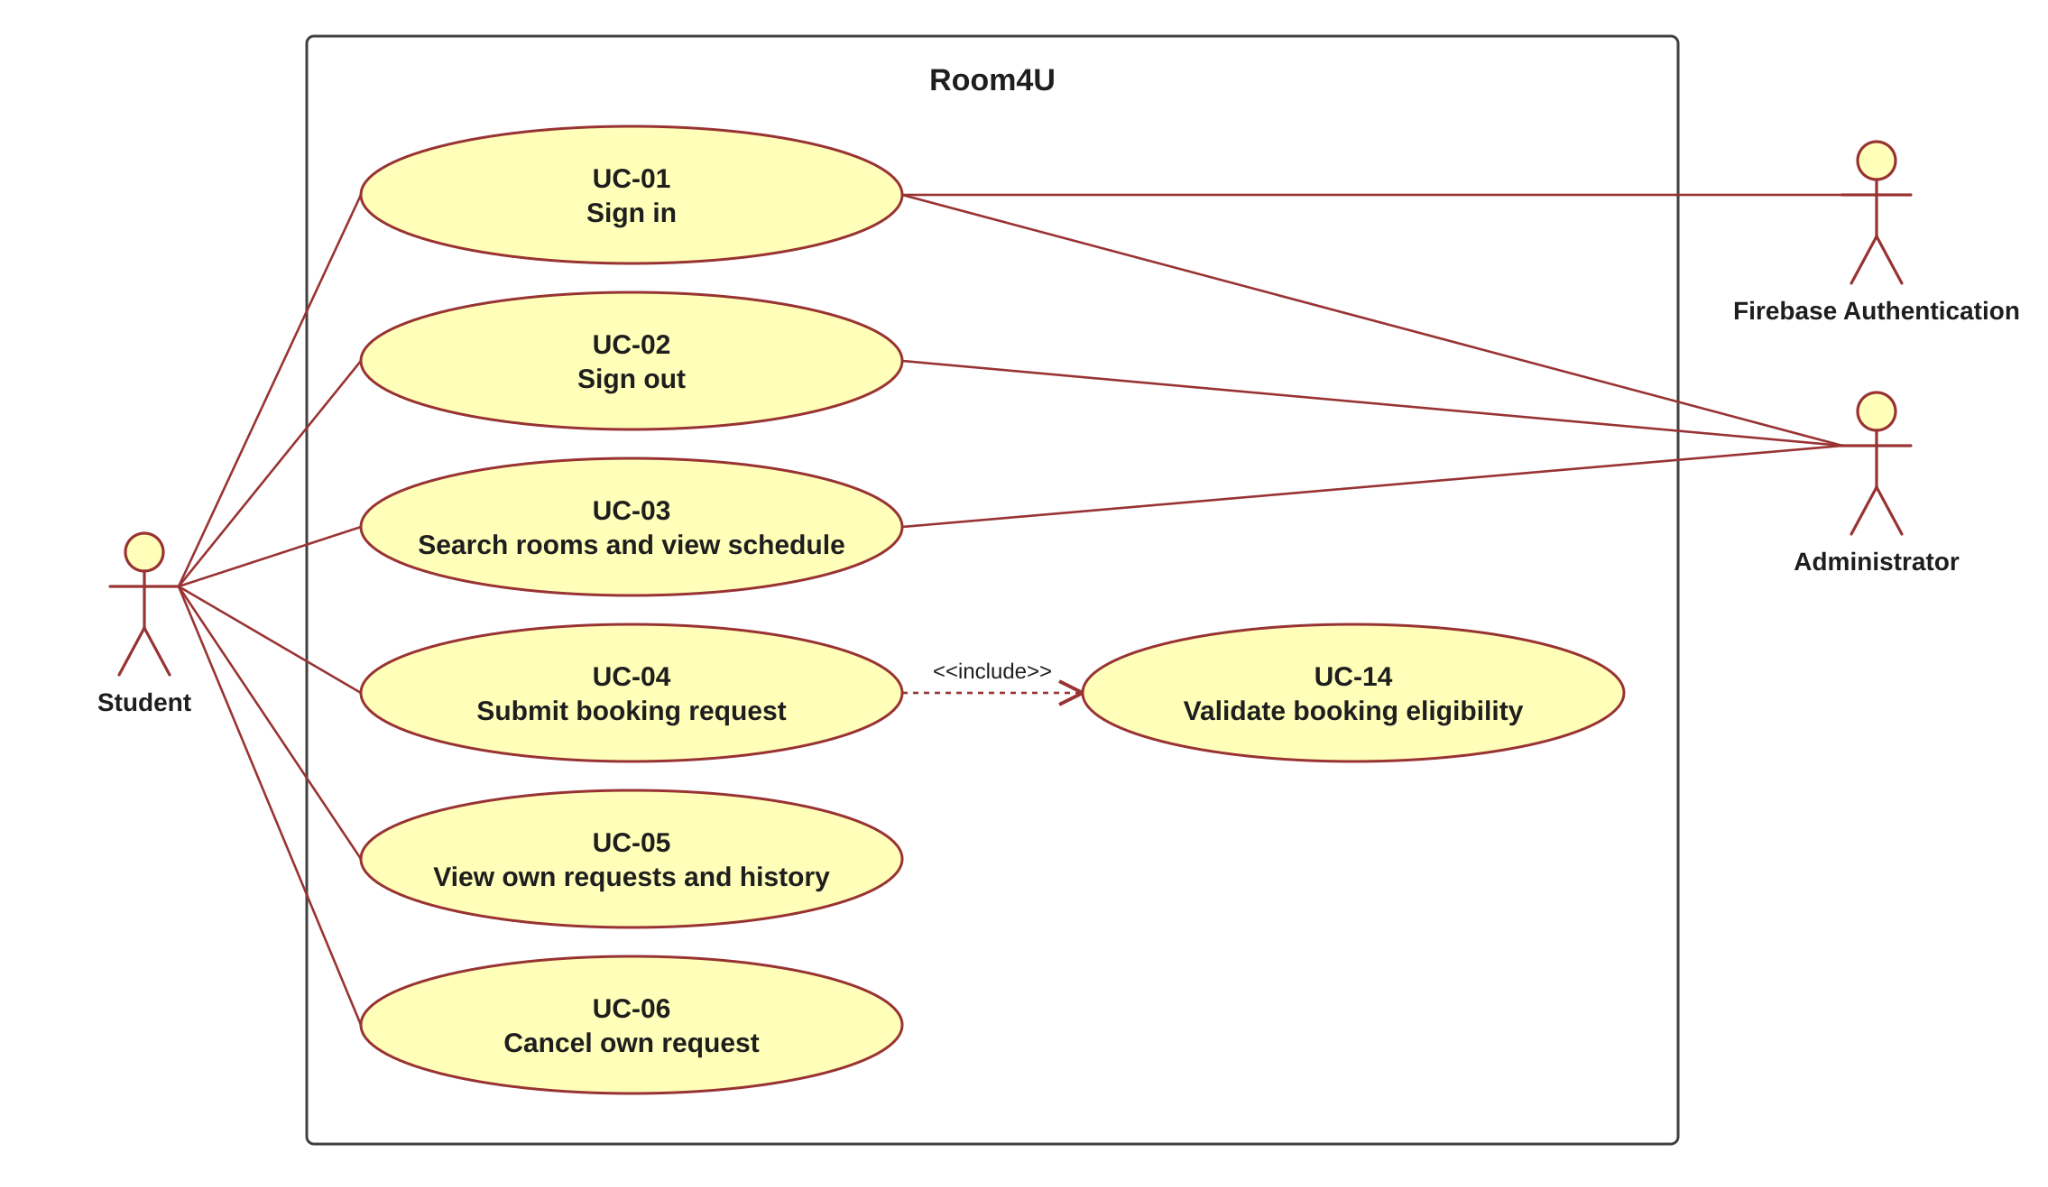
\includegraphics[width=\textwidth,height=0.68\textheight,keepaspectratio]{images/use-case-student.png}
\caption{Student workflows and shared session and room access. The dashed include arrow points from UC-04 to UC-14 because each submission validates eligibility. UC-14 is internal included behavior and has no direct user association. Preconditions such as sign-in are not modeled as repeated include relationships.}
\end{figure}

\begin{figure}[H]
\centering
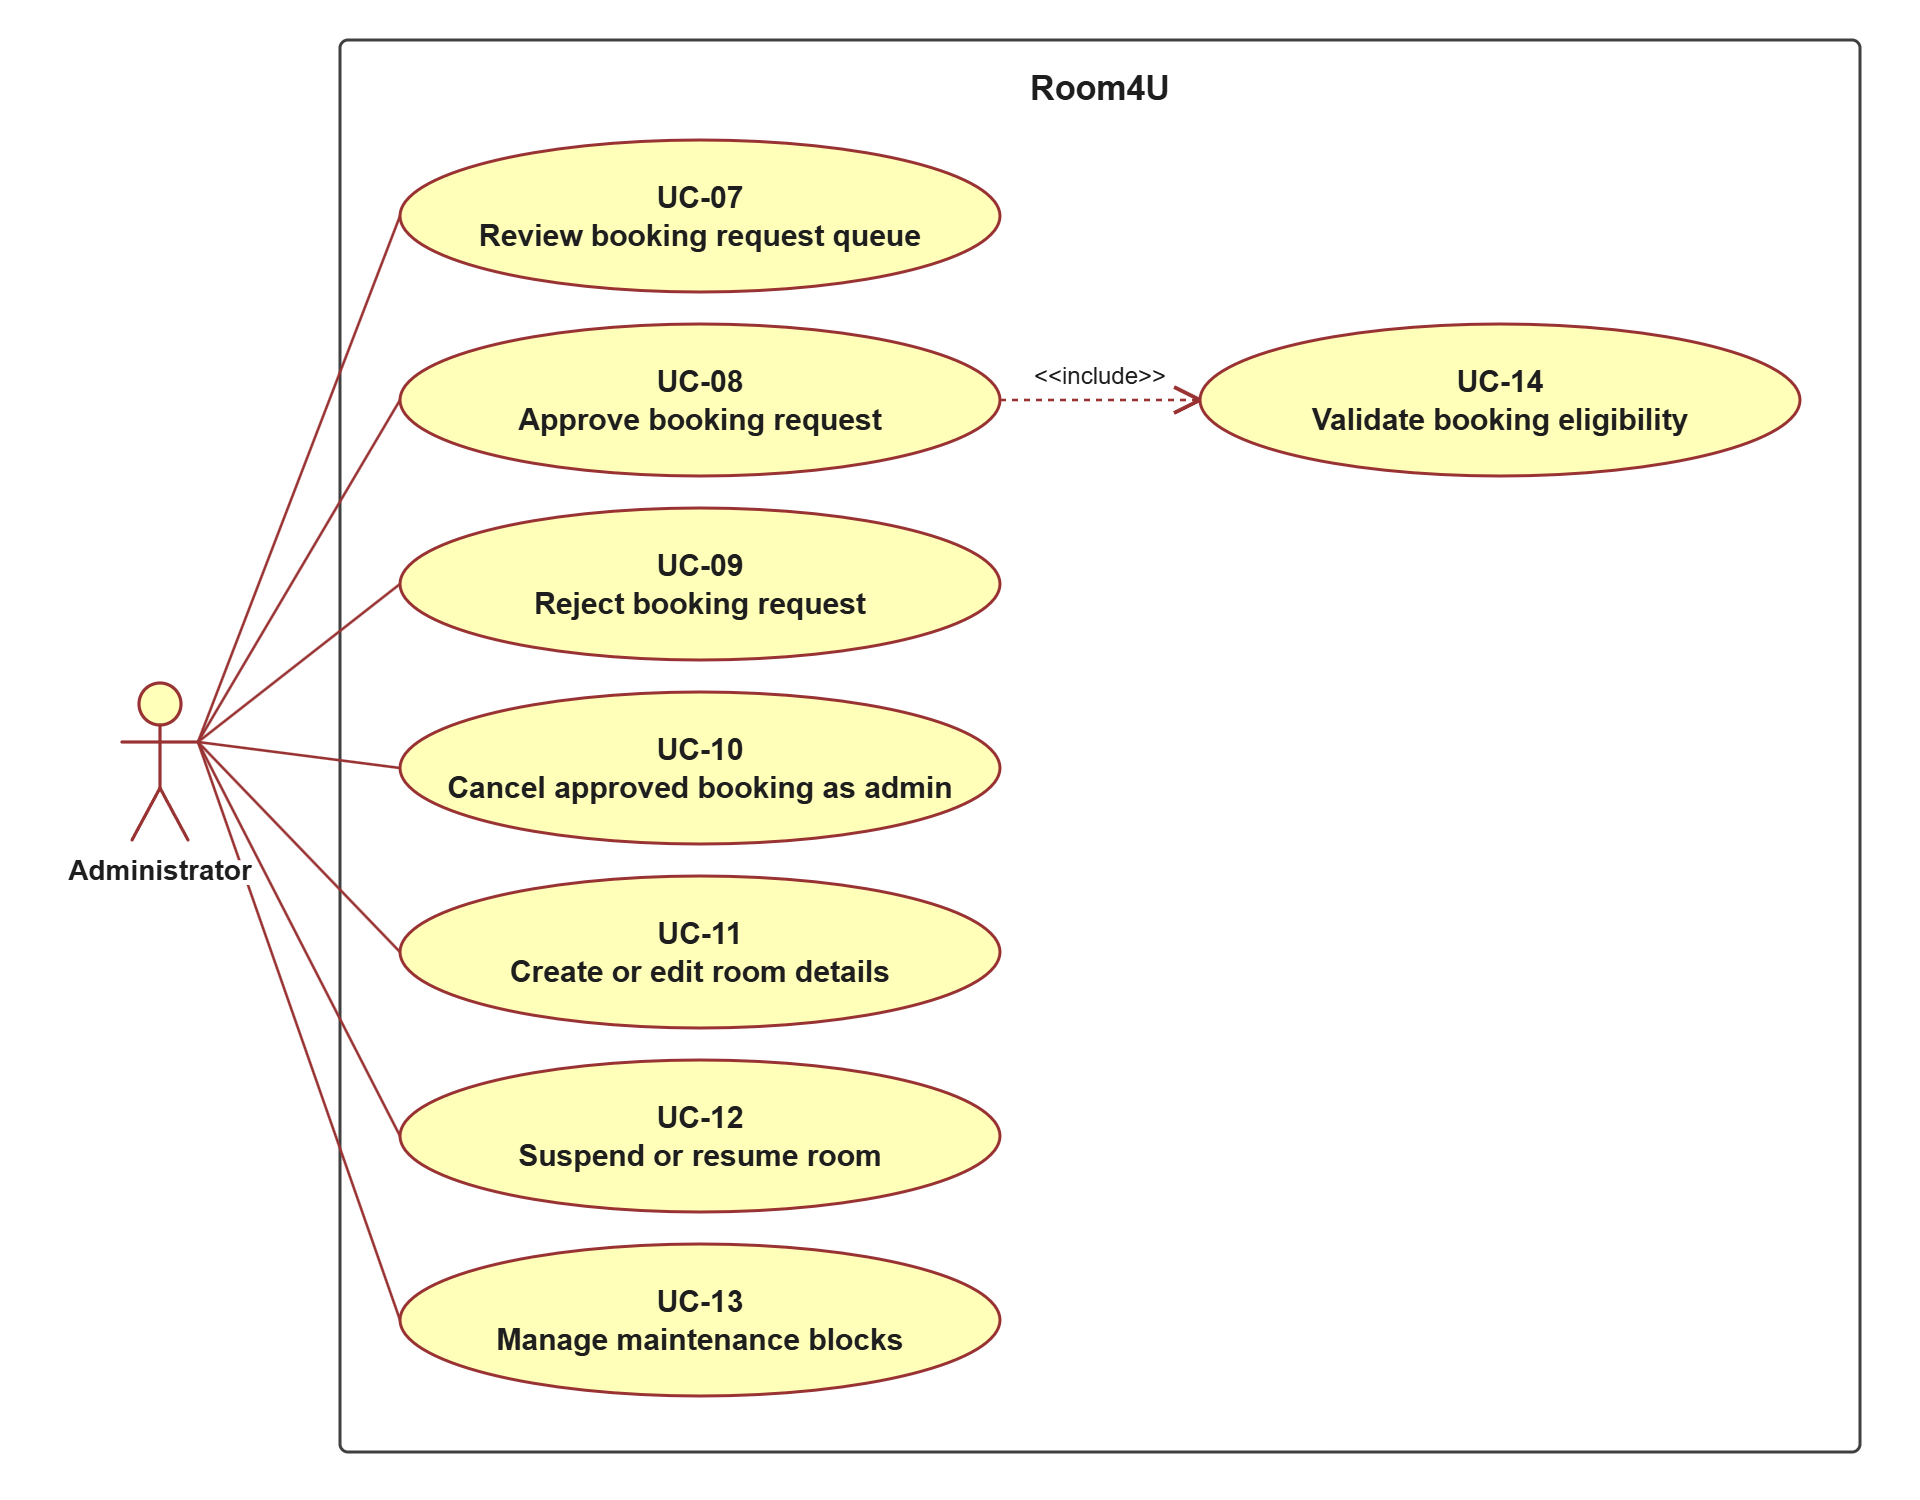
\includegraphics[width=\textwidth,height=0.68\textheight,keepaspectratio]{images/use-case-administrator.png}
\caption{Administrator workflows for requests, rooms and maintenance. UC-08 includes UC-14 for each approval. Rejection, cancellation and maintenance management are separate user goals, not unconditional includes of approval. No extend relationship or actor generalization is needed for the specified behavior.}
\end{figure}

\subsection{Actors}
\begin{srstable}{p{0.25\textwidth}|L}
\textbf{Actor} & \textbf{Responsibilities} \\ \hline
Student & Uses an account created in advance; searches rooms and views schedules; submits, views and cancels only the Student's own booking requests. \\ \hline
Administrator & Reviews, approves, rejects and cancels booking requests; manages rooms and maintenance blocks; and searches rooms and views schedules. An Administrator may work in several windows at the same time. \\ \hline
Firebase Authentication & External system that checks a user's sign-in credentials. It participates in UC-01 only; Room4U determines the user's role and permitted access. \\ \hline
\end{srstable}

The backend and PostgreSQL are internal parts of Room4U, not use-case actors. The instructor and TA are project stakeholders, not product actors.

\subsection{Use Case List}
\begingroup
\small
\setstretch{1.0}
\setlength{\tabcolsep}{3pt}
\renewcommand{\arraystretch}{1.1}
\begin{longtable}{|>{\raggedright\arraybackslash}p{0.40\textwidth}|>{\raggedright\arraybackslash}p{0.20\textwidth}|>{\raggedright\arraybackslash}p{0.12\textwidth}|>{\raggedright\arraybackslash}p{0.23\textwidth}|}
\hline
\textbf{ID and use case} & \textbf{Primary actor} & \textbf{Priority} & \textbf{Related FR} \\ \hline
\endfirsthead
\hline
\textbf{ID and use case} & \textbf{Primary actor} & \textbf{Priority} & \textbf{Related FR} \\ \hline
\endhead
\hline
\endfoot
\hline
\endlastfoot
UC-01 Sign in & Student or Administrator & Must & FR-01--FR-03 \\ \hline
UC-02 Sign out & Student or Administrator & Must & FR-05 \\ \hline
UC-03 Search rooms and view schedule & Student or Administrator & Must & FR-06--FR-09, FR-27 \\ \hline
UC-04 Submit booking request & Student & Must & FR-10--FR-11, FR-19 \\ \hline
UC-05 View own requests and history & Student & Must & FR-04, FR-12, FR-19 \\ \hline
UC-06 Cancel own request & Student & Must & FR-04, FR-13, FR-19 \\ \hline
UC-07 Review booking request queue & Administrator & Must & FR-03, FR-14, FR-19 \\ \hline
UC-08 Approve booking request & Administrator & Must & FR-15--FR-16, FR-19 \\ \hline
UC-09 Reject booking request & Administrator & Must & FR-17, FR-19 \\ \hline
UC-10 Cancel approved booking as administrator & Administrator & Must & FR-18--FR-19 \\ \hline
UC-11 Create or edit room details & Administrator & Must & FR-20--FR-21, FR-27 \\ \hline
UC-12 Suspend or resume room & Administrator & Must & FR-16, FR-22--FR-23, FR-27 \\ \hline
UC-13 Manage maintenance blocks & Administrator & Must & FR-16, FR-24--FR-27 \\ \hline
UC-14 Validate booking eligibility & None (included by UC-04 and UC-08) & Included Must & FR-10, FR-15--FR-16, FR-22 \\ \hline
\end{longtable}
\endgroup

\clearpage
\section{Use Case Specifications}

All listed use cases are Must-have. Student and Administrator accounts are pre-created. Firebase Authentication is the supporting external actor only in UC-01; the database and backend are internal parts of Room4U. Decisions D01--D08 are accepted in the reviewed requirements baseline; these specifications do not claim that the described functionality has been implemented or tested.

FR-02, FR-03 and NFR-02 apply as cross-cutting constraints to every protected action, including UC-04--UC-06. Room4U checks the current identity and application role; Student request operations also verify ownership. UC-14 inherits authentication and authorization from its caller, UC-04 or UC-08, and has no independent actor or screen. UC-02 can clear local private state when a session has expired. State-changing actions recheck the current record before committing. A failed or refused write leaves status, availability and required history unchanged. Pending requests do not reserve a room; Approved bookings and active maintenance blocks do. Intervals are half-open: they conflict only when each interval starts before the other ends, so adjacent intervals are allowed.

\Needspace{6\baselineskip}
\begin{usecasebox}{UC-01 Sign in}
\noindent\textbf{Primary actor:} Student or Administrator.\quad
\textbf{Supporting actor:} Firebase Authentication.\quad
\textbf{Priority:} Must.\par
\textbf{Trace:} FR-01--03; BR-01; NFR-02, NFR-04, NFR-06--07, NFR-12; Screen S01.\par
\textbf{Trigger:} The user chooses Sign in.\par
\textbf{Preconditions:} A pre-created account exists. An active Room4U session is not required; connectivity is handled at run time.\par
\textbf{Success postcondition:} Room4U establishes the user's application role and opens the corresponding home view.\par
\textbf{Failure postcondition:} No application session or protected data is granted.\par
\textbf{Main flow}
\begin{enumerate}[label=\arabic*.,leftmargin=2em,itemsep=1pt,topsep=2pt]
  \item The user opens the sign-in screen.
  \item The user enters the account email and password and submits the form.
  \item Firebase Authentication verifies the credentials.
  \item Room4U validates the returned identity and loads the account's application role.
  \item Room4U opens the Student room view or the Administrator request queue according to that role.
\end{enumerate}
\Needspace{3\baselineskip}
\textbf{Alternative flows}
\begin{itemize}[label={},leftmargin=0pt,itemsep=1pt,topsep=1pt]
  \item \textbf{A1 (at step 1):} If a valid Room4U session already exists, the system opens the role-appropriate home view.
\end{itemize}
\Needspace{3\baselineskip}
\textbf{Exception flows}
\begin{itemize}[label={},leftmargin=0pt,itemsep=1pt,topsep=1pt]
  \item \textbf{E1 (at step 3):} Invalid credentials produce a generic error and allow the user to retry without revealing whether the account exists.
  \item \textbf{E2 (at steps 3--4):} A network failure, invalid identity or missing application role prevents access and displays a retry or sign-in message.
\end{itemize}
\end{usecasebox}

\Needspace{6\baselineskip}
\begin{usecasebox}{UC-02 Sign out}
\noindent\textbf{Primary actor:} Student or Administrator.\quad
\textbf{Supporting actor:} None.\quad
\textbf{Priority:} Must.\par
\textbf{Trace:} FR-05; BR-16; NFR-02, NFR-06--07, NFR-12; Screens S02--S08.\par
\textbf{Trigger:} The user chooses Sign out.\par
\textbf{Preconditions:} A Room4U application session is active, or local private state remains after session expiry.\par
\textbf{Success postcondition:} The client session and private view are cleared; subsequent protected operations require sign-in.\par
\textbf{Failure postcondition:} The interface does not re-expose private data after sign-out is requested.\par
\textbf{Main flow}
\begin{enumerate}[label=\arabic*.,leftmargin=2em,itemsep=1pt,topsep=2pt]
  \item The user chooses Sign out from the authenticated navigation.
  \item Room4U displays a confirmation dialog over the current view with Cancel and Log Out actions.
  \item The user confirms by choosing Log Out.
  \item Room4U clears the current client identity and private cached view.
  \item Room4U opens the sign-in screen.
  \item When the user later requests a protected operation, Room4U requires a valid session.
\end{enumerate}
\Needspace{3\baselineskip}
\textbf{Alternative flows}
\begin{itemize}[label={},leftmargin=0pt,itemsep=1pt,topsep=1pt]
  \item \textbf{A1 (at step 3):} If the user chooses Cancel or closes the dialog, Room4U closes it and leaves the session and current screen unchanged; the use case ends.
  \item \textbf{A2 (at step 1):} If the session has already expired, Room4U clears the local private view and opens the sign-in screen; the use case ends.
\end{itemize}
\Needspace{3\baselineskip}
\textbf{Exception flows}
\begin{itemize}[label={},leftmargin=0pt,itemsep=1pt,topsep=1pt]
  \item \textbf{E1 (at step 4):} If the network is unavailable, Room4U still clears local private state and opens the sign-in screen; it does not claim to revoke a token copied outside the client.
\end{itemize}
\end{usecasebox}

\Needspace{6\baselineskip}
\begin{usecasebox}{UC-03 Search rooms and view schedule}
\noindent\textbf{Primary actor:} Student or Administrator.\quad
\textbf{Supporting actor:} None.\quad
\textbf{Priority:} Must.\par
\textbf{Trace:} FR-06--09, FR-27; BR-05--07, BR-16; NFR-01--02, NFR-04--05, NFR-07, NFR-12; Screen S02.\par
\textbf{Trigger:} The user opens Rooms or changes a search filter.\par
\textbf{Preconditions:} The user is signed in.\par
\textbf{Success postcondition:} Matching rooms and the selected room's current schedule are visible without exposing another student's identity.\par
\textbf{Failure postcondition:} No room, booking or maintenance data is changed.\par
\textbf{Main flow}
\begin{enumerate}[label=\arabic*.,leftmargin=2em,itemsep=1pt,topsep=2pt]
  \item The user selects a booking date and enters a group size.
  \item Room4U validates the filter values.
  \item Room4U lists matching rooms with stable identity, name, capacity, equipment, image or placeholder, and availability state.
  \item The user opens a room's schedule for the selected date.
  \item Room4U displays Approved occupancy and active maintenance intervals, omits Pending requests as reservations, and hides other students' personal details.
\end{enumerate}
\Needspace{3\baselineskip}
\textbf{Alternative flows}
\begin{itemize}[label={},leftmargin=0pt,itemsep=1pt,topsep=1pt]
  \item \textbf{A1 (at step 3):} If no room matches, Room4U shows an empty state and lets the user change the filters.
  \item \textbf{A2 (at step 5):} If the selected room is suspended, Room4U labels it and does not offer a valid new-request path for that room.
\end{itemize}
\Needspace{3\baselineskip}
\textbf{Exception flows}
\begin{itemize}[label={},leftmargin=0pt,itemsep=1pt,topsep=1pt]
  \item \textbf{E1 (at step 2):} Invalid filter values receive field-level errors; no search result is presented as valid.
  \item \textbf{E2 (at steps 3--5):} A load failure shows a retry state and is not presented as an empty result or a free schedule.
\end{itemize}
\end{usecasebox}

\Needspace{6\baselineskip}
\begin{usecasebox}{UC-04 Submit booking request}
\noindent\textbf{Primary actor:} Student.\quad
\textbf{Supporting actor:} None.\quad
\textbf{Priority:} Must.\par
\textbf{Trace:} FR-10--11, FR-19, FR-27; BR-01--07, BR-09, BR-11; NFR-02, NFR-04--05, NFR-07, NFR-09--12; Screens S03--S04.\par
\textbf{Trigger:} The student chooses Request room.\par
\textbf{Preconditions:} The student is signed in and has selected a room. Eligibility is checked at submission time rather than assumed from the earlier search.\par
\textbf{Success postcondition:} One uniquely identified Pending request and its creation event exist; the request does not reserve the interval.\par
\textbf{Failure postcondition:} No request or history event is created.\par
\textbf{Main flow}
\begin{enumerate}[label=\arabic*.,leftmargin=2em,itemsep=1pt,topsep=2pt]
  \item Room4U shows the selected room, booking rules and time zone.
  \item The student enters the date, start time, duration and group size.
  \item The student confirms the request.
  \item Room4U includes UC-14 to validate the current room, time, capacity and availability.
  \item Room4U creates the Pending request and its creation event as one consistent outcome; the interval remains available unless another Approved booking or maintenance block occupies it.
  \item Room4U shows the request ID and explains that administrator approval is still required.
\end{enumerate}
\Needspace{3\baselineskip}
\textbf{Alternative flows}
\begin{itemize}[label={},leftmargin=0pt,itemsep=1pt,topsep=1pt]
  \item \textbf{A1 (at step 2):} The student changes the selected room and returns to search without submitting.
\end{itemize}
\Needspace{3\baselineskip}
\textbf{Exception flows}
\begin{itemize}[label={},leftmargin=0pt,itemsep=1pt,topsep=1pt]
  \item \textbf{E1 (at step 4):} Invalid input, a suspended room, an Approved overlap or active maintenance prevents submission; Room4U identifies the issue and preserves valid form values.
  \item \textbf{E2 (at step 5):} If persistence fails, neither the request nor its event is committed; Room4U does not show a request ID or claim success.
\end{itemize}
\end{usecasebox}

\Needspace{6\baselineskip}
\begin{usecasebox}{UC-05 View own requests and history}
\noindent\textbf{Primary actor:} Student.\quad
\textbf{Supporting actor:} None.\quad
\textbf{Priority:} Must.\par
\textbf{Trace:} FR-04, FR-12, FR-19; BR-09, BR-16; NFR-01--02, NFR-04--05, NFR-07, NFR-10, NFR-12; Screen S04.\par
\textbf{Trigger:} The student opens My requests.\par
\textbf{Preconditions:} The student is signed in.\par
\textbf{Success postcondition:} The student sees only their own request details and ordered history.\par
\textbf{Failure postcondition:} No request belonging to another student is disclosed.\par
\textbf{Main flow}
\begin{enumerate}[label=\arabic*.,leftmargin=2em,itemsep=1pt,topsep=2pt]
  \item The student opens My requests.
  \item Room4U retrieves requests owned by the authenticated student only.
  \item The student selects one of their requests.
  \item Room4U shows its room, time, group size, status, ordered history and any recorded processing or cancellation reason.
  \item The student may refresh to retrieve newer committed data.
\end{enumerate}
\Needspace{3\baselineskip}
\textbf{Alternative flows}
\begin{itemize}[label={},leftmargin=0pt,itemsep=1pt,topsep=1pt]
  \item \textbf{A1 (at step 2):} If the student has no requests, Room4U shows an empty state and a link to room search.
\end{itemize}
\Needspace{3\baselineskip}
\textbf{Exception flows}
\begin{itemize}[label={},leftmargin=0pt,itemsep=1pt,topsep=1pt]
  \item \textbf{E1 (at step 3):} A direct link to another owner's request is denied without returning its private details.
  \item \textbf{E2 (at steps 2--5):} A load failure offers retry and is not presented as a successful current result.
\end{itemize}
\end{usecasebox}

\Needspace{6\baselineskip}
\begin{usecasebox}{UC-06 Cancel own request}
\noindent\textbf{Primary actor:} Student.\quad
\textbf{Supporting actor:} None.\quad
\textbf{Priority:} Must.\par
\textbf{Trace:} FR-04, FR-13, FR-19; BR-09--10, BR-12; NFR-02, NFR-04, NFR-07, NFR-09--12; Screen S04.\par
\textbf{Trigger:} The owner chooses Cancel request.\par
\textbf{Preconditions:} The student is signed in and is the request owner. Current status and start-time eligibility are rechecked during the flow.\par
\textbf{Success postcondition:} An eligible request becomes Cancelled, a transition event is retained, and any Approved interval is released.\par
\textbf{Failure postcondition:} Status, occupancy and history remain unchanged.\par
\textbf{Main flow}
\begin{enumerate}[label=\arabic*.,leftmargin=2em,itemsep=1pt,topsep=2pt]
  \item The student opens their request and chooses Cancel.
  \item Room4U presents the room and time details and asks for confirmation.
  \item The student confirms.
  \item Room4U rechecks ownership, current Pending or Approved status, and that the booking start is still in the future.
  \item Room4U records Cancelled with a transition event and refreshes the request view; if the request was Approved, its interval is released.
\end{enumerate}
\Needspace{3\baselineskip}
\textbf{Alternative flows}
\begin{itemize}[label={},leftmargin=0pt,itemsep=1pt,topsep=1pt]
  \item \textbf{A1 (at step 3):} If the student declines confirmation, Room4U leaves the request unchanged.
\end{itemize}
\Needspace{3\baselineskip}
\textbf{Exception flows}
\begin{itemize}[label={},leftmargin=0pt,itemsep=1pt,topsep=1pt]
  \item \textbf{E1 (at step 4):} A started request or a Rejected or Cancelled request cannot be cancelled again.
  \item \textbf{E2 (at step 4):} If another session has changed the request, Room4U refuses the stale action, refreshes the view and reports the current status.
  \item \textbf{E3 (at step 5):} A persistence failure preserves the prior status, occupancy and history.
\end{itemize}
\end{usecasebox}

\Needspace{6\baselineskip}
\begin{usecasebox}{UC-07 Review booking request queue}
\noindent\textbf{Primary actor:} Administrator.\quad
\textbf{Supporting actor:} None.\quad
\textbf{Priority:} Must.\par
\textbf{Trace:} FR-14, FR-19; BR-09, BR-16; NFR-02, NFR-07, NFR-12; Screens S05--S06.\par
\textbf{Trigger:} The Administrator opens Booking requests.\par
\textbf{Preconditions:} The user is signed in with the Administrator role.\par
\textbf{Success postcondition:} The Administrator sees the current request queue and details for a selected request; no request is processed by viewing it.\par
\textbf{Failure postcondition:} No request status or history is changed.\par
\textbf{Main flow}
\begin{enumerate}[label=\arabic*.,leftmargin=2em,itemsep=1pt,topsep=2pt]
  \item The Administrator opens the booking request queue.
  \item Room4U defaults to Pending and offers status filters, including Approved, with room, time, group size and submission time.
  \item The Administrator selects a request.
  \item Room4U shows the current request history and the room's current availability.
  \item Room4U offers only the processing actions permitted by the request's current status.
\end{enumerate}
\Needspace{3\baselineskip}
\textbf{Alternative flows}
\begin{itemize}[label={},leftmargin=0pt,itemsep=1pt,topsep=1pt]
  \item \textbf{A1 (at step 2):} If there are no Pending requests, Room4U shows an empty queue.
\end{itemize}
\Needspace{3\baselineskip}
\textbf{Exception flows}
\begin{itemize}[label={},leftmargin=0pt,itemsep=1pt,topsep=1pt]
  \item \textbf{E1 (at step 4):} If the selected item is stale or already processed, Room4U shows its latest state and refreshes the queue.
  \item \textbf{E2 (at steps 1--5):} A user without the Administrator role is denied access.
  \item \textbf{E3 (at steps 2--4):} A load failure is reported with a retry option and is not shown as an empty queue.
\end{itemize}
\end{usecasebox}

\Needspace{6\baselineskip}
\begin{usecasebox}{UC-08 Approve booking request}
\noindent\textbf{Primary actor:} Administrator.\quad
\textbf{Supporting actor:} None.\quad
\textbf{Priority:} Must.\par
\textbf{Trace:} FR-15--16, FR-19, FR-27; BR-02--09, BR-11; NFR-02--04, NFR-07, NFR-09--12; Screen S06.\par
\textbf{Trigger:} The Administrator chooses Approve for a request.\par
\textbf{Preconditions:} The Administrator is signed in and has opened a request. Eligibility is not assumed from the displayed details.\par
\textbf{Success postcondition:} One eligible request becomes Approved, reserves its interval and has a corresponding history event.\par
\textbf{Failure postcondition:} No conflicting booking or partial status, availability or history change is committed.\par
\textbf{Main flow}
\begin{enumerate}[label=\arabic*.,leftmargin=2em,itemsep=1pt,topsep=2pt]
  \item The Administrator reviews the request and chooses Approve.
  \item Room4U asks the Administrator to confirm the decision.
  \item The Administrator confirms.
  \item Room4U rechecks that the request is Pending and includes UC-14 using current committed data for time, room state, capacity and occupancy.
  \item Room4U commits Approved status, the reservation and its history as one atomic outcome.
  \item Room4U displays the outcome and updates the queue and room schedule.
\end{enumerate}
\Needspace{3\baselineskip}
\textbf{Alternative flows}
\begin{itemize}[label={},leftmargin=0pt,itemsep=1pt,topsep=1pt]
  \item \textbf{A1 (at step 3):} If the Administrator declines confirmation, Room4U makes no change.
\end{itemize}
\Needspace{3\baselineskip}
\textbf{Exception flows}
\begin{itemize}[label={},leftmargin=0pt,itemsep=1pt,topsep=1pt]
  \item \textbf{E1 (at steps 4--5):} If a concurrent approval or maintenance operation wins the conflict, this request remains Pending and Room4U reports the conflict.
  \item \textbf{E2 (at step 4):} If the request is no longer Pending, its start is no longer eligible, the room is suspended or its capacity is insufficient, Room4U refuses approval and reports the cause.
  \item \textbf{E3 (at step 5):} A write failure leaves the prior status, occupancy and history intact.
\end{itemize}
\end{usecasebox}

\Needspace{6\baselineskip}
\begin{usecasebox}{UC-09 Reject booking request}
\noindent\textbf{Primary actor:} Administrator.\quad
\textbf{Supporting actor:} None.\quad
\textbf{Priority:} Must.\par
\textbf{Trace:} FR-17, FR-19; BR-09--10, BR-13; NFR-02, NFR-07, NFR-09--12; Screens S04, S06.\par
\textbf{Trigger:} The Administrator chooses Reject.\par
\textbf{Preconditions:} The Administrator is signed in and has opened a request.\par
\textbf{Success postcondition:} A Pending request becomes Rejected and its valid reason is retained in the owner's history.\par
\textbf{Failure postcondition:} The current status and history remain unchanged.\par
\textbf{Main flow}
\begin{enumerate}[label=\arabic*.,leftmargin=2em,itemsep=1pt,topsep=2pt]
  \item The Administrator chooses Reject and enters a reason.
  \item Room4U trims and validates the reason as nonblank and 1--250 characters.
  \item The Administrator confirms rejection.
  \item Room4U rechecks that the request is Pending.
  \item Room4U records Rejected, its transition event and reason, then refreshes the queue.
\end{enumerate}
\Needspace{3\baselineskip}
\textbf{Alternative flows}
\begin{itemize}[label={},leftmargin=0pt,itemsep=1pt,topsep=1pt]
  \item \textbf{A1 (at step 3):} If the Administrator cancels the confirmation, Room4U leaves the request status and history unchanged; the use case ends.
  \item \textbf{A2 (at step 4):} If the request is still Pending but its start time has passed, rejection remains allowed; continue at step 5.
\end{itemize}
\Needspace{3\baselineskip}
\textbf{Exception flows}
\begin{itemize}[label={},leftmargin=0pt,itemsep=1pt,topsep=1pt]
  \item \textbf{E1 (at step 2):} A blank or overlong reason receives a field error. Room4U preserves the entered reason and makes no status or history change; return to step 1 to correct it.
  \item \textbf{E2 (at step 4):} If a concurrent action has already processed the request, Room4U refuses the stale rejection, displays the current status and refreshes the queue. No transition or history event is added; the use case ends.
  \item \textbf{E3 (at step 5):} A persistence failure leaves the request and history unchanged.
\end{itemize}
\end{usecasebox}

\Needspace{6\baselineskip}
\begin{usecasebox}{UC-10 Cancel approved booking as admin}
\noindent\textbf{Primary actor:} Administrator.\quad
\textbf{Supporting actor:} None.\quad
\textbf{Priority:} Must.\par
\textbf{Trace:} FR-18--19; BR-09--10, BR-12--13, BR-15; NFR-02, NFR-07, NFR-09--12; Screens S04, S06.\par
\textbf{Trigger:} The Administrator opens an Approved booking and chooses Cancel.\par
\textbf{Preconditions:} The Administrator is signed in; the booking is accessible from request details or an affected-booking link.\par
\textbf{Success postcondition:} A future Approved booking becomes Cancelled, its interval is released and the reason and history remain visible to authorized users.\par
\textbf{Failure postcondition:} The booking, occupancy and history remain unchanged.\par
\textbf{Main flow}
\begin{enumerate}[label=\arabic*.,leftmargin=2em,itemsep=1pt,topsep=2pt]
  \item The Administrator reviews the Approved booking details.
  \item The Administrator enters a cancellation reason and confirms.
  \item Room4U validates the reason, current Approved status and that the booking start is still in the future.
  \item Room4U records Cancelled with its transition event and reason, and releases the interval as one consistent outcome.
  \item The owner can see the cancellation reason in My requests.
\end{enumerate}
\Needspace{3\baselineskip}
\textbf{Alternative flows}
\begin{itemize}[label={},leftmargin=0pt,itemsep=1pt,topsep=1pt]
  \item \textbf{A1 (at step 2):} If the Administrator abandons cancellation, Room4U makes no change.
\end{itemize}
\Needspace{3\baselineskip}
\textbf{Exception flows}
\begin{itemize}[label={},leftmargin=0pt,itemsep=1pt,topsep=1pt]
  \item \textbf{E1 (at step 3):} An invalid reason, a booking that has started, or a changed status prevents cancellation.
  \item \textbf{E2 (at step 4):} A write failure preserves the prior status, reservation and history.
\end{itemize}
\end{usecasebox}

\Needspace{6\baselineskip}
\begin{usecasebox}{UC-11 Create or edit room details}
\noindent\textbf{Primary actor:} Administrator.\quad
\textbf{Supporting actor:} None.\quad
\textbf{Priority:} Must.\par
\textbf{Trace:} FR-20--21, FR-27; BR-05, BR-14; NFR-02, NFR-07, NFR-09, NFR-11--12; Screen S07.\par
\textbf{Trigger:} The Administrator chooses Add room or Edit room.\par
\textbf{Preconditions:} The Administrator is signed in. An existing room is selected for an edit.\par
\textbf{Success postcondition:} Valid room details are saved and available to later room queries; an edit retains the stable room ID.\par
\textbf{Failure postcondition:} No invalid room or partial edit is stored; existing details remain intact.\par
\textbf{Main flow}
\begin{enumerate}[label=\arabic*.,leftmargin=2em,itemsep=1pt,topsep=2pt]
  \item The Administrator opens a new-room form or an existing room.
  \item The Administrator enters the room code, name, capacity and equipment description, and may select a preloaded photo.
  \item Room4U validates field limits, room-code uniqueness after trimming and case-insensitive comparison, and the capacity range.
  \item For an edit, Room4U preserves the room ID and checks that the proposed capacity still accommodates every future Approved group in that room.
  \item The Administrator chooses Save. Room4U revalidates the fields, room-code uniqueness and, for an edit, the proposed capacity against all future Approved bookings using current data. These checks and the save form one consistent operation so concurrent approvals cannot violate the room-capacity constraint. Room4U saves valid details, retains the room ID on edit and displays the result.
\end{enumerate}
\Needspace{3\baselineskip}
\textbf{Alternative flows}
\begin{itemize}[label={},leftmargin=0pt,itemsep=1pt,topsep=1pt]
  \item \textbf{A1 (at step 1):} For an edit, Room4U loads existing values and retains the stable room ID.
  \item \textbf{A2 (at step 2):} If no photo is selected, Room4U uses the placeholder image.
\end{itemize}
\Needspace{3\baselineskip}
\textbf{Exception flows}
\begin{itemize}[label={},leftmargin=0pt,itemsep=1pt,topsep=1pt]
  \item \textbf{E1 (at steps 3 or 5):} Invalid fields or a duplicate room code prevent saving. Room4U identifies invalid fields and preserves valid form values; return to step 2.
  \item \textbf{E2 (at steps 4 or 5):} If the proposed capacity is below the group size of a future Approved booking, including one approved concurrently, Room4U refuses the edit and leaves stored room and booking data unchanged; return to step 2.
  \item \textbf{E3 (at step 5):} A persistence failure prevents saving. No partial room change is committed; Room4U preserves entered form values and reports the failure. The Administrator may retry from step 5 or leave without saving.
\end{itemize}
\end{usecasebox}

\Needspace{6\baselineskip}
\begin{usecasebox}{UC-12 Suspend or resume room}
\noindent\textbf{Primary actor:} Administrator.\quad
\textbf{Supporting actor:} None.\quad
\textbf{Priority:} Must.\par
\textbf{Trace:} FR-16, FR-22--23, FR-27; BR-08, BR-11; NFR-02--03, NFR-07, NFR-09, NFR-11--12; Screen S07.\par
\textbf{Trigger:} The Administrator chooses Suspend or Resume.\par
\textbf{Preconditions:} The Administrator is signed in.\par
\textbf{Success postcondition:} The room's active/suspended state changes consistently; existing Approved bookings and maintenance remain retained.\par
\textbf{Failure postcondition:} No partial availability change occurs.\par
\textbf{Main flow}
\begin{enumerate}[label=\arabic*.,leftmargin=2em,itemsep=1pt,topsep=2pt]
  \item The Administrator opens Room Management, selects a room and chooses Suspend.
  \item Room4U explains that suspension blocks new submissions and approvals but preserves existing Approved bookings and maintenance.
  \item The Administrator confirms suspension.
  \item Room4U atomically rechecks the current room state and sets it to suspended, consistently with concurrent approvals. An approval committed before suspension remains valid; an approval after suspension fails. Existing Approved bookings and maintenance blocks remain unchanged.
  \item Subsequent searches, submissions and approval checks reflect the new room state.
\end{enumerate}
\Needspace{3\baselineskip}
\textbf{Alternative flows}
\begin{itemize}[label={},leftmargin=0pt,itemsep=1pt,topsep=1pt]
  \item \textbf{A1 (at step 1):} If the selected room is suspended, the Administrator chooses Resume instead of Suspend.
  \item \textbf{A1.1:} The Administrator selects Resume.
  \item \textbf{A1.2:} Room4U explains that new submissions and approvals will be allowed again, subject to booking rules and existing occupancy.
  \item \textbf{A1.3:} The Administrator confirms.
  \item \textbf{A1.4:} Room4U rechecks that the room is still suspended and changes it to active, preserving all existing Approved bookings and maintenance blocks.
  \item \textbf{A1.5:} Continue at main-flow step 5, then end the use case.
  \item \textbf{A2 (at main-flow step 3 or A1.3):} If the Administrator declines confirmation, the room state, bookings and maintenance blocks remain unchanged; the use case ends.
\end{itemize}
\Needspace{3\baselineskip}
\textbf{Exception flows}
\begin{itemize}[label={},leftmargin=0pt,itemsep=1pt,topsep=1pt]
  \item \textbf{E1 (at step 4 or A1.4):} If the room state has changed since it was displayed, Room4U refuses the stale action, shows the current state and refreshes the view. The use case ends; the Administrator may start a new action using refreshed data.
  \item \textbf{E2 (at step 4 or A1.4):} A persistence failure prevents the state change. No partial change is committed; the prior room state, bookings and maintenance blocks remain intact. Room4U reports the failure and the use case ends.
\end{itemize}
\end{usecasebox}

\Needspace{6\baselineskip}
\begin{usecasebox}{UC-13 Manage maintenance blocks}
\noindent\textbf{Primary actor:} Administrator.\quad
\textbf{Supporting actor:} None.\quad
\textbf{Priority:} Must.\par
\textbf{Trace:} FR-16, FR-24--27; BR-06--08, BR-13, BR-15; NFR-02--03, NFR-07, NFR-09, NFR-11--12; Screens S06, S08.\par
\textbf{Trigger:} The Administrator chooses Add maintenance or Remove block.\par
\textbf{Preconditions:} The Administrator is signed in and has selected a room.\par
\textbf{Success postcondition:} A valid non-conflicting block is added, or an eligible future block is removed with its record retained; other occupancy is preserved.\par
\textbf{Failure postcondition:} No maintenance record or booking is partially changed.\par
\textbf{Main flow}
\begin{enumerate}[label=\arabic*.,leftmargin=2em,itemsep=1pt,topsep=2pt]
  \item The Administrator enters the room, maintenance start and end, and reason.
  \item Room4U validates that the end is later than the start and that the trimmed reason contains 1--250 characters.
  \item Room4U checks current Approved bookings and active maintenance intervals for the selected room.
  \item The Administrator confirms creation.
  \item Room4U rechecks the conflicts and commits the maintenance block and its retained record as one consistent outcome.
  \item Room4U updates room schedules and subsequent submission and approval checks.
\end{enumerate}
\Needspace{3\baselineskip}
\textbf{Alternative flows}
\begin{itemize}[label={},leftmargin=0pt,itemsep=1pt,topsep=1pt]
  \item \textbf{A1 (at step 1):} Remove a future maintenance block.
  \item \textbf{A1.1:} The Administrator selects an existing maintenance block.
  \item \textbf{A1.2:} Room4U displays its room, interval, reason and current state, then asks for confirmation of removal.
  \item \textbf{A1.3:} The Administrator confirms removal.
  \item \textbf{A1.4:} Room4U rechecks with current server time and data that the block still exists, is active and has not started.
  \item \textbf{A1.5:} Room4U marks the block removed and retains its record. Removal does not change any booking or other maintenance block.
  \item \textbf{A1.6:} Room4U refreshes the schedule and availability. Only the removed block ceases to restrict the interval; all other occupancy and room-state restrictions still apply. The use case ends.
  \item \textbf{A2 (at step 3):} If an Approved booking conflicts with the proposed maintenance interval, the Administrator opens the affected booking and performs UC-10. After successful cancellation, continue at main-flow step 2 to revalidate the interval and recheck all conflicts. If cancellation is declined or fails, no maintenance block is created and the use case ends.
  \item \textbf{A3 (at step 4 or A1.3):} If the Administrator declines confirmation, no maintenance or booking data changes; the use case ends.
\end{itemize}
\Needspace{3\baselineskip}
\textbf{Exception flows}
\begin{itemize}[label={},leftmargin=0pt,itemsep=1pt,topsep=1pt]
  \item \textbf{E1 (at step 2):} An invalid interval or reason prevents creation. Room4U identifies the invalid fields and preserves valid form values; return to step 1.
  \item \textbf{E2 (at steps 3 or 5):} An Approved booking overlap, overlapping active maintenance block or competing approval prevents creation. Room4U identifies the conflict and commits no new block; the Administrator may revise the interval from step 1 or follow A2 to resolve an affected booking.
  \item \textbf{E3 (at A1.4):} If the selected block no longer exists, has already been removed or has started, Room4U refuses removal and refreshes the displayed data. No maintenance or booking record changes; the use case ends.
  \item \textbf{E4 (at step 5 or A1.5):} A persistence failure prevents creation or removal. No partial change is committed; existing maintenance and booking records remain unchanged. Room4U reports the failure and the use case ends.
\end{itemize}
\end{usecasebox}

\Needspace{6\baselineskip}
\begin{usecasebox}{UC-14 Validate booking eligibility}
\noindent\textbf{Primary actor:} None (included internal behavior).\par
\textbf{Supporting actor:} None.\quad\textbf{Priority:} Must.\par
\textbf{Trace:} FR-10, FR-15--16, FR-27; BR-01--08, BR-11; NFR-02--03, NFR-09, NFR-11; Screens S03, S06.\par
\textbf{Trigger:} UC-04 or UC-08 requests eligibility validation.\par
\textbf{Preconditions:} The calling use case has authenticated and authorized its actor; candidate request fields and current room data are available.\par
\textbf{Success postcondition:} Eligibility is returned to the caller for that operation; this included behavior does not itself create or transition a request.\par
\textbf{Failure postcondition:} A specific violated rule is returned and no booking state changes.\par
\textbf{Main flow}
\begin{enumerate}[label=\arabic*.,leftmargin=2em,itemsep=1pt,topsep=2pt]
  \item Room4U checks that the selected room exists and currently accepts submissions or approvals for the requested action.
  \item Room4U validates date, start time, duration, advance limit and group size against the current room capacity.
  \item Room4U checks current Approved bookings and active maintenance for overlap using the defined interval boundaries.
  \item Room4U returns the eligibility result to UC-04 or UC-08; for approval, the caller commits only if the current validation and approval remain one atomic decision.
\end{enumerate}
\Needspace{3\baselineskip}
\textbf{Alternative flows}
\begin{itemize}[label={},leftmargin=0pt,itemsep=1pt,topsep=1pt]
  \item \textbf{A1 (at step 3):} Overlapping Pending requests are ignored because they do not reserve room capacity.
\end{itemize}
\Needspace{3\baselineskip}
\textbf{Exception flows}
\begin{itemize}[label={},leftmargin=0pt,itemsep=1pt,topsep=1pt]
  \item \textbf{E1 (at steps 1--3):} If a rule fails or the current data is no longer eligible, Room4U returns the cause to the caller and leaves all records unchanged.
\end{itemize}
\end{usecasebox}

\section{Prototype / Mockups}

This section presents the Room4U user-interface prototypes and mockups.
The screens illustrate the layout, information hierarchy, navigation,
and main interactions of the system. Room4U provides two role-based
interfaces: the Student Interface and the Administrator Interface. Both
use the Room4U open-book logo and a consistent blue-and-white visual
language, including the account bar, left navigation, room information
panels, status indicators, and primary action buttons. The mockups
communicate the intended appearance and behavior of the system before
implementation.

The following subsections describe the interactive prototypes, screen
list, individual mockups, key confirmation and result dialogs, and
accessibility considerations.

\section*{9.1. Interactive Prototype}\label{interactive-prototype}
\addcontentsline{toc}{section}{9.1. Interactive Prototype}

Room4U provides separate navigation flows for Student and Administrator
roles. The Student prototype covers room discovery, availability
checking, booking submission, request tracking, request details,
cancellation, history, and logout. The Administrator prototype covers
request processing, room management, room creation and editing, room
suspension and resumption, room-usage schedules, and maintenance
scheduling.

\begin{itemize}
\item
  Student Interactive Prototype: Students can search for meeting rooms,
  inspect room information and availability, submit booking requests,
  review request statuses and details, cancel eligible requests, view
  processed requests, and log out.

  \begin{itemize}
  \item
    \textbf{Prototype Link:}
    \href{https://www.figma.com/proto/0kLDFGO5txhnNfoH99CaKa/Room4U---Version-3?node-id=7-4}{Figma Student Prototype}
  \end{itemize}
\item
  Administrator Interactive Prototype: Administrators can review and
  process booking requests, approve or reject pending requests, cancel
  approved bookings when permitted, manage room information, suspend or
  resume rooms, inspect room usage, and create or remove maintenance
  schedules. The interface also provides confirmation, success, and
  validation dialogs for important actions.

  \begin{itemize}
  \item
    \textbf{Prototype Link:}
    \href{https://www.figma.com/proto/0kLDFGO5txhnNfoH99CaKa/Room4U---Version-3?node-id=51-239}{Figma Administrator Prototype}
  \end{itemize}
\end{itemize}

\section*{9.2. Screen List and Mockups}\label{screen-list-and-mockups}
\addcontentsline{toc}{section}{9.2. Screen List and Mockups}

This subsection lists the main Room4U screens and their associated use
cases. The screens are grouped by user role. Each entry identifies the
screen's purpose and summarizes the information,
actions, and important interaction states represented by the mockups.

\subsection*{Screen List}
\addcontentsline{toc}{subsection}{Screen List}
\label{screen-list}

\begin{longtable}{|p{0.16\textwidth}|p{0.39\textwidth}|p{0.35\textwidth}|}
\hline
\textbf{Screen ID} & \textbf{Screen Name} & \textbf{Related Use Case(s)} \\
\hline
\endfirsthead
\hline
\textbf{Screen ID} & \textbf{Screen Name} & \textbf{Related Use Case(s)} \\
\hline
\endhead
S01 & Sign In & UC-01 \\
\hline
S02 & Room Search and Availability & UC-02, UC-03 \\
\hline
S03 & Booking Request & UC-04 \\
\hline
S04 & My Requests, Details and History & UC-02, UC-05, UC-06 \\
\hline
S05 & Admin Request Queue & UC-02, UC-07 \\
\hline
S06 & Request Details and Processing & UC-07, UC-08, UC-09, UC-10 \\
\hline
S07 & Room Management & UC-11, UC-12 \\
\hline
S08 & Room Availability and Maintenance & UC-13 \\
\hline
\end{longtable}

\section*{9.2.1. Student Interface}\label{student-interface}
\addcontentsline{toc}{section}{9.2.1. Student Interface}

The Student Interface supports the complete student-side booking flow.
Students can sign in, search for rooms, inspect availability, submit a
booking request, monitor its status, open request details, cancel an
eligible request, review request history, and log out.

\subsection*{9.2.1.1. S01 - Sign In}\label{s01---sign-in}
\addcontentsline{toc}{subsection}{9.2.1.1. S01 - Sign In}

\begin{itemize}
\item
  Description: This screen is the entry point for both Student and
  Administrator users. It provides Email and Password fields and a Sign
  In button. Users sign in with accounts provided by the system; no
  public registration flow is shown. The screen includes Room4U branding
  and a short explanation of the service. If authentication fails, an
  error message is displayed so the user can check the credentials and
  try again.
\item
  \textbf{Mockup View:}
\end{itemize}

\begin{quote}
\begin{center}
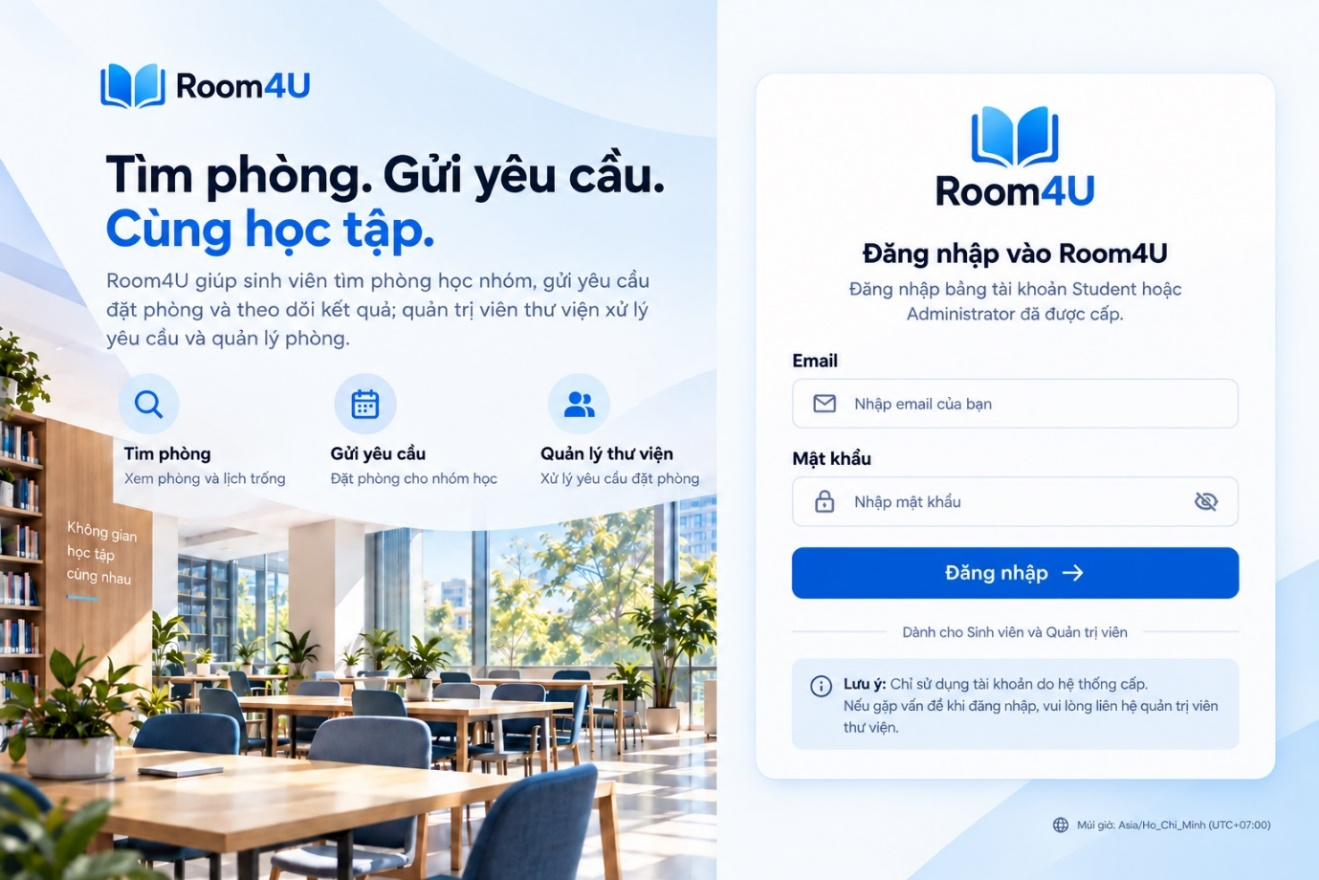
\includegraphics[width=0.9\textwidth,height=0.72\textheight,keepaspectratio]{images/image1.jpeg}
\end{center}
\end{quote}

\subsection*{9.2.1.2. S02 - Room Search and
Availability}\label{s02---room-search-and-availability}
\addcontentsline{toc}{subsection}{9.2.1.2. S02 - Room Search and
Availability}

\begin{itemize}
\item
  Description: This flow helps students find a suitable meeting room and
  check its schedule before submitting a booking request. It consists of
  room-search results and a room-availability view.

  \begin{itemize}
  \item
    Room Search: Students can search using available criteria such as
    the intended date, number of people, and room requirements. Results
    are presented as room cards showing a room image, room name,
    capacity, floor, equipment, current status, and an action to inspect
    the room or its availability.
  \item
    Room Availability: After selecting a room, students can view its
    time-slot schedule for a selected date. The schedule distinguishes
    available periods from approved bookings, maintenance periods, and
    other unavailable periods so that students can choose a valid time
    before opening the booking-request form.
  \end{itemize}
\item
  \textbf{Mockup Views:}
\end{itemize}

\subsubsection*{S02.1 -- Room Search}
\addcontentsline{toc}{subsubsection}{S02.1 -- Room Search}

\begin{center}
\begin{center}
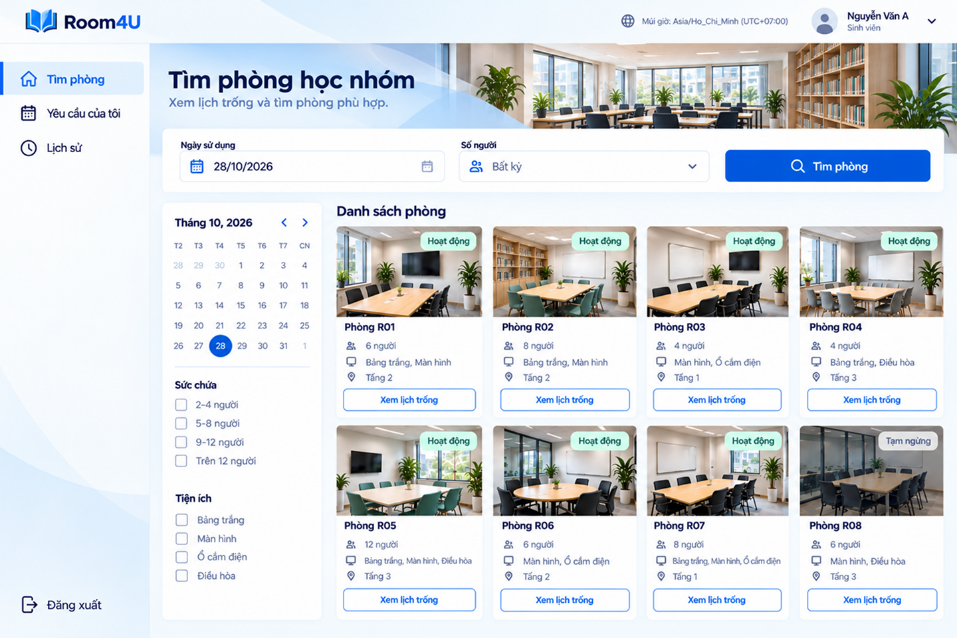
\includegraphics[width=0.9\textwidth,height=0.72\textheight,keepaspectratio]{images/image2.png}
\end{center}
\end{center}

\subsubsection{S02.2 -- Room
Availability}\label{s02.2-room-availability}

\begin{quote}
\begin{center}
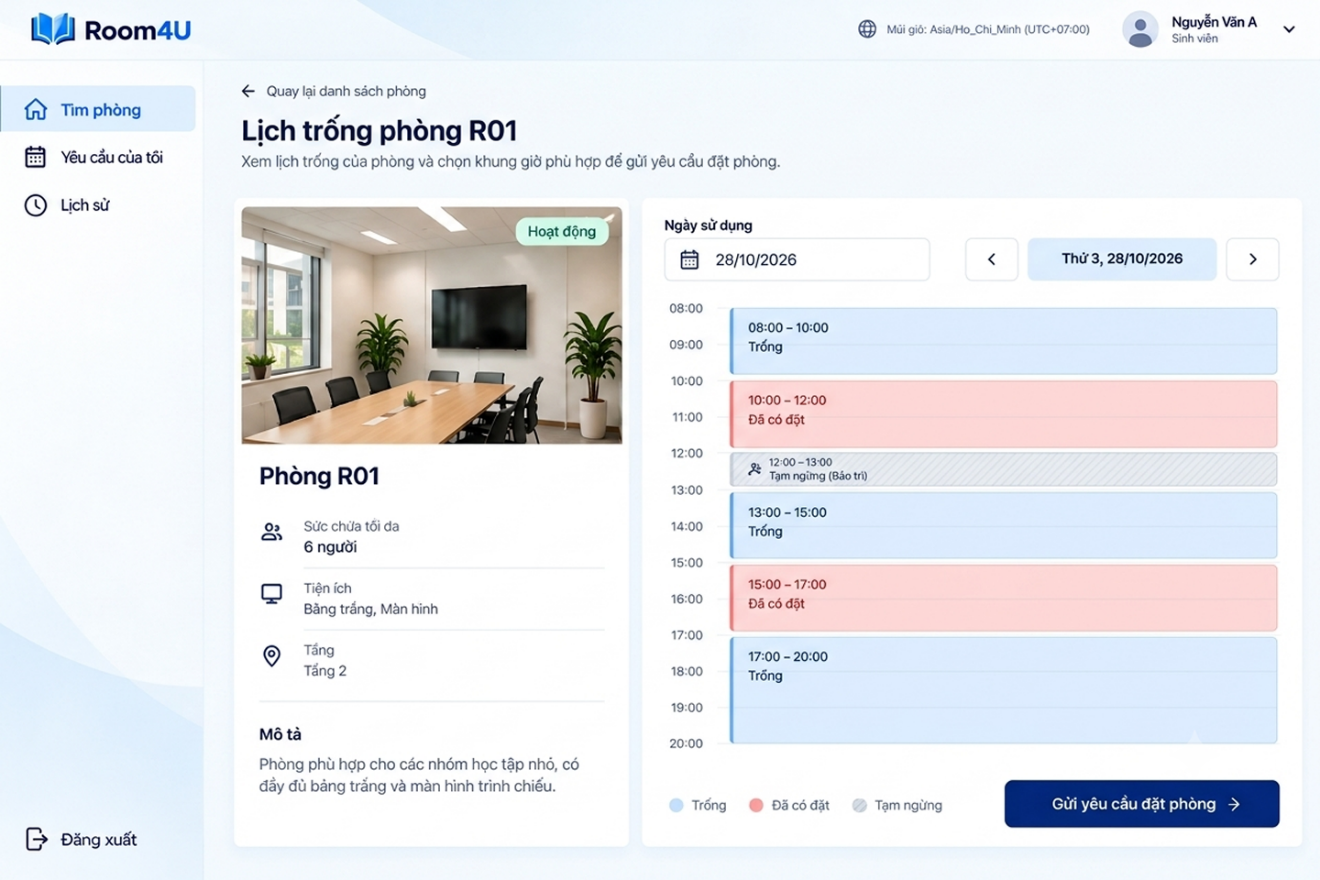
\includegraphics[width=0.9\textwidth,height=0.72\textheight,keepaspectratio]{images/image3.png}
\end{center}
\end{quote}

\subsection*{9.2.1.3. S03 - Booking
Request}\label{s03---booking-request}
\addcontentsline{toc}{subsection}{9.2.1.3. S03 - Booking Request}

\begin{itemize}
\item
  Description: This screen allows a student to submit a booking request
  for the selected room. The form displays the room information and
  collects the usage date, start time, duration, number of participants,
  purpose of use, and an optional note. The available duration options
  are 30, 60, 90, and 120 minutes. The system calculates the end time
  from the selected start time and duration and displays it for the
  student to review. The start time must be later than the current time
  and no more than seven days from the current time (BR-04). The system
  validates the request against room capacity, availability, and the
  applicable booking rules. A successfully submitted request receives a
  request ID and appears with Pending status in the
  student's request list.
\item
  \textbf{Mockup View:}
\end{itemize}

\begin{center}
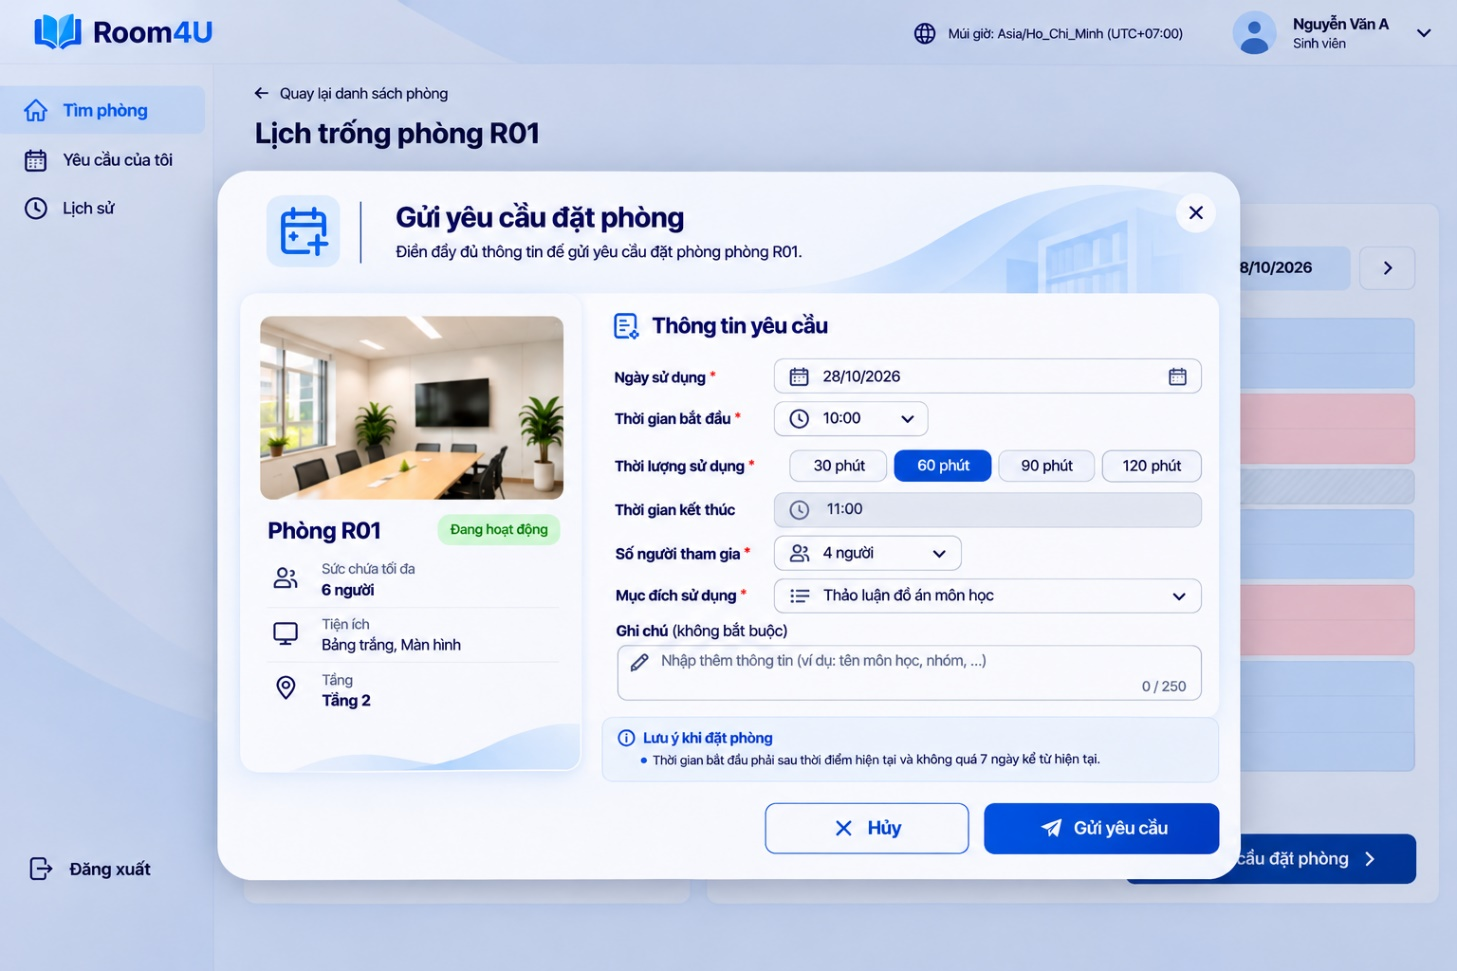
\includegraphics[width=0.9\textwidth,height=0.72\textheight,keepaspectratio]{images/image4.jpeg}
\end{center}

\begin{center}
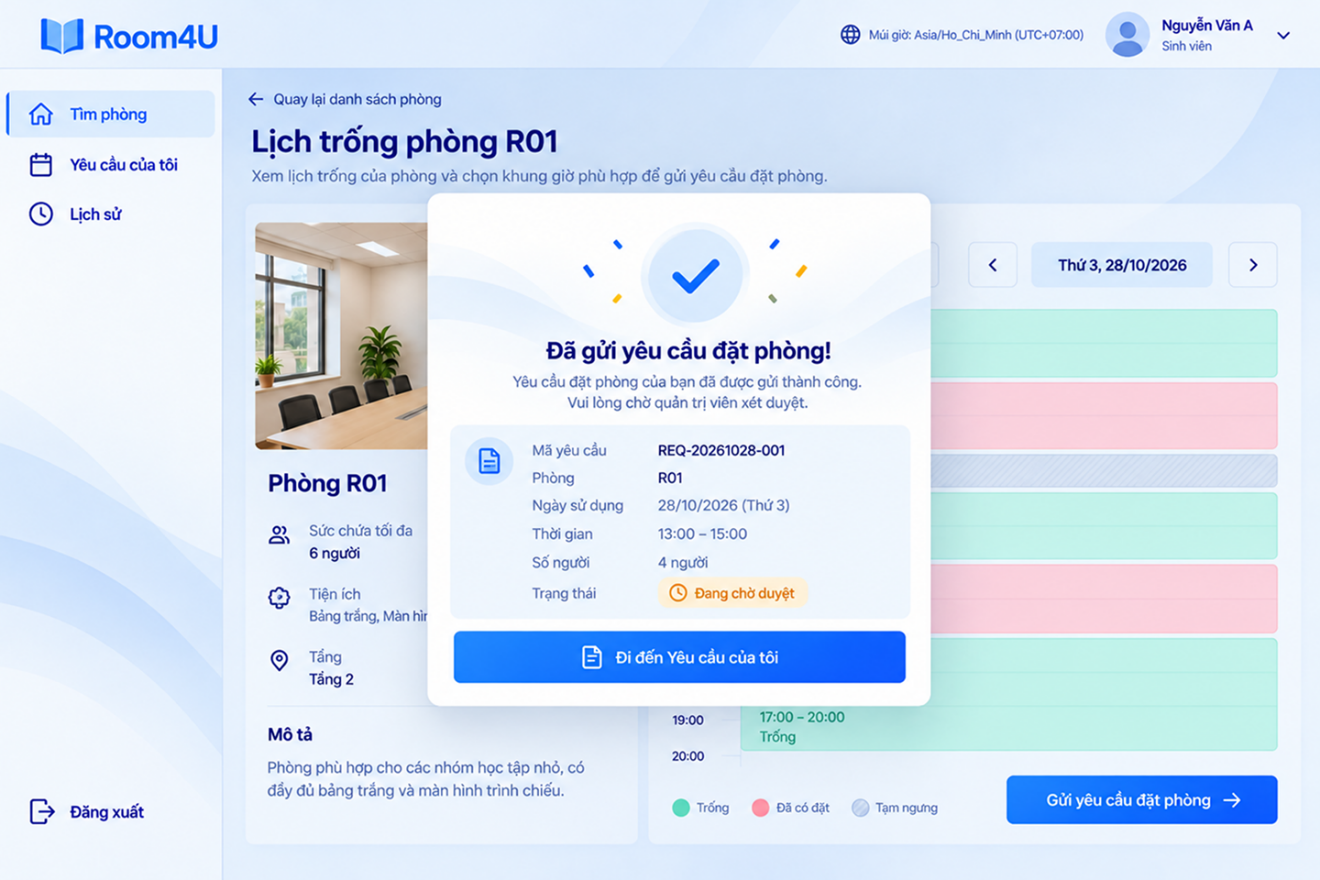
\includegraphics[width=0.9\textwidth,height=0.72\textheight,keepaspectratio]{images/image5.png}
\end{center}

\subsection*{9.2.1.4. S04 - My Requests and
History}\label{s04---my-requests-and-history}
\addcontentsline{toc}{subsection}{9.2.1.4. S04 - My Requests and
History}

\begin{itemize}
\item
  Description: This area allows students to monitor submitted booking
  requests and review requests that have already been processed. The
  active-request screen provides search and status filters. Each row
  shows the request ID, room, usage date and time, purpose, current
  status, and a View Details action. Students can open a request to
  inspect its full information. A separate History screen lists
  previously processed requests.
\end{itemize}

\subsection*{9.2.1.4.1. S04.1 - My Requests
List}\label{s04.1---my-requests-list}
\addcontentsline{toc}{subsection}{9.2.1.4.1. S04.1 - My Requests List}

This screen displays the student's request list. Status
tabs help students narrow the results, while the search field supports
searching by request ID, room, or purpose. The table presents the
request ID, room, usage date and time, purpose, status, and a View
Details action. Pagination is provided when the results exceed one page.

\begin{itemize}
\item
  \textbf{Mockup View :}
\end{itemize}

\begin{center}
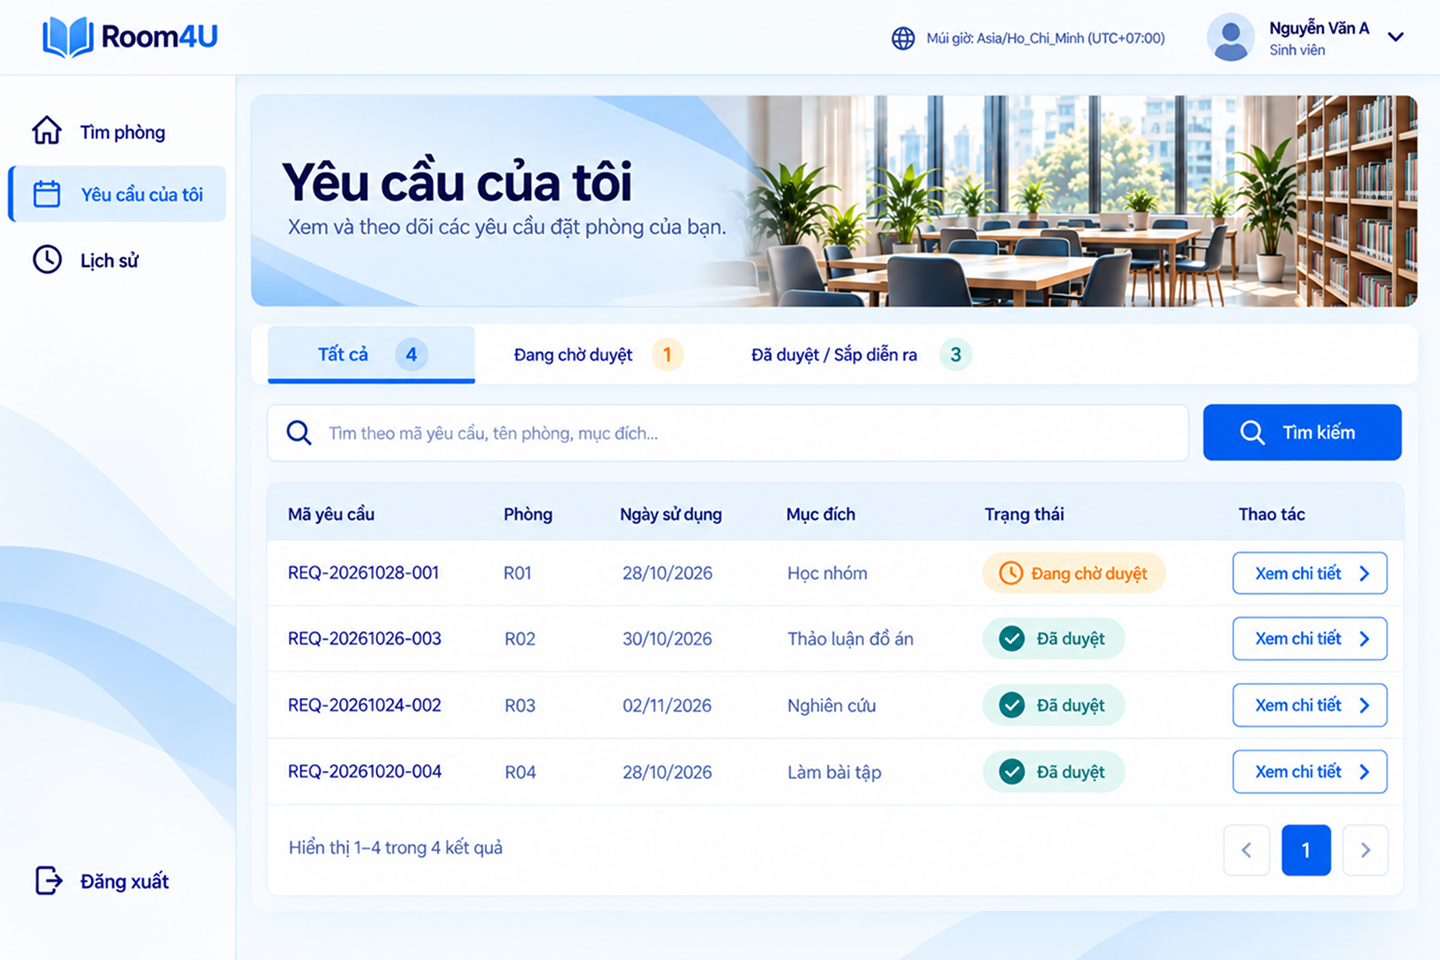
\includegraphics[width=0.9\textwidth,height=0.72\textheight,keepaspectratio]{images/image6.png}
\end{center}

\subsection*{9.2.1.4.2. S04.2 - Booking Request
Details}\label{s04.2---booking-request-details}
\addcontentsline{toc}{subsection}{9.2.1.4.2. S04.2 - Booking Request
Details}

This screen presents the full information for one selected request. It
includes the request ID and current status, room information, usage date
and time, number of participants, purpose, optional note, and requester
information. The student can use Cancel Request when cancellation is
permitted. Cancellation is subject to the applicable request-status and
booking-time rules; it is not an unconditional action.

\begin{itemize}
\item
  \textbf{Mockup View:}
\end{itemize}

\begin{quote}
\begin{center}
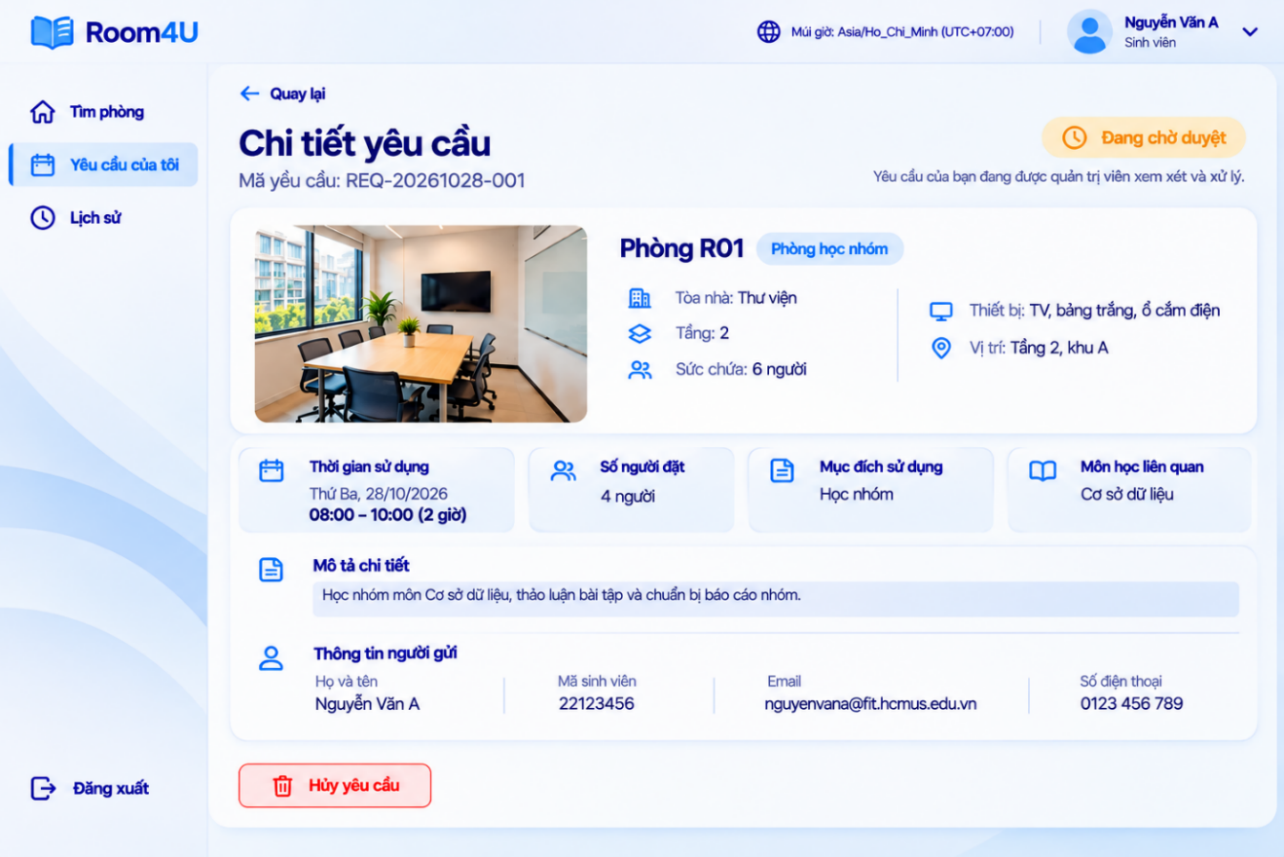
\includegraphics[width=0.9\textwidth,height=0.72\textheight,keepaspectratio]{images/image7.png}
\end{center}
\end{quote}

Cancellation Interaction: When a student selects Cancel Request for an
eligible request, the system asks for confirmation before changing the
request status. If cancellation is not allowed, the interface explains
why the action cannot proceed. Closing the dialog or choosing not to
continue leaves the request unchanged.

History Function: The History screen allows students to review
previously processed booking requests. It includes Rejected and
Cancelled requests, as well as Approved requests whose scheduled usage
time has passed. An approved request retains its Approved status; the
interface may indicate that its scheduled time has passed rather than
changing the status to Completed. The history table shows the request
ID, room, usage date, purpose, status, and a View Details action. Search
and pagination help students locate older records.

Logout Interaction: The Logout option is available in the left
navigation. Selecting it opens a confirmation dialog over the current
page. The dialog provides Cancel and Log Out actions. Cancel closes the
dialog and keeps the student on the current page; Log Out ends the
session and returns the user to the Sign In screen.

\begin{itemize}
\item
  Mockup View -- History Page with Logout Confirmation:
\end{itemize}

\begin{center}
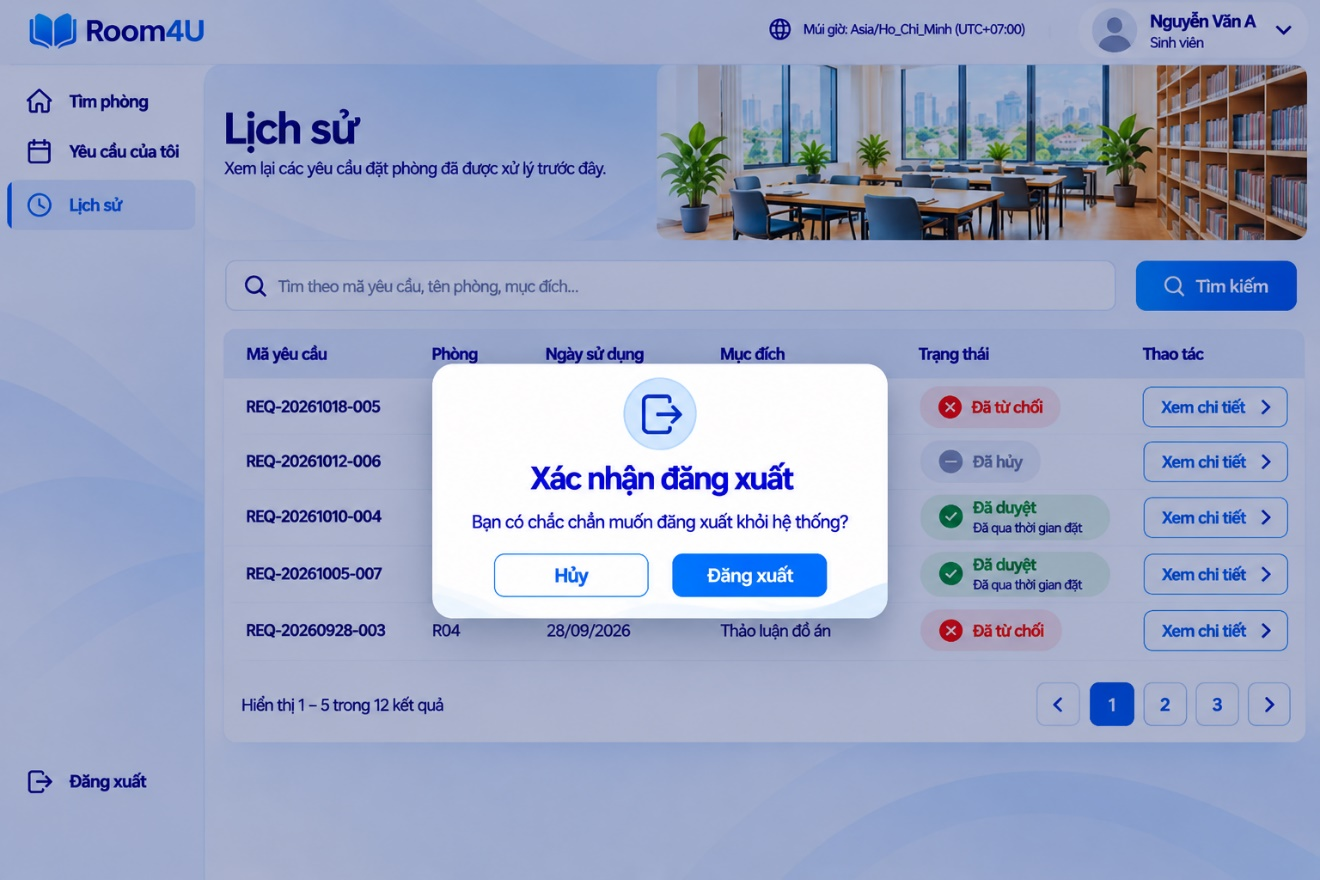
\includegraphics[width=0.9\textwidth,height=0.72\textheight,keepaspectratio]{images/image8.jpeg}
\end{center}

\section*{9.2.2. Administrator Interface}\label{administrator-interface}
\addcontentsline{toc}{section}{9.2.2. Administrator Interface}

The Administrator Interface supports the management and supervision of
Room4U operations. Administrators can review and process student booking
requests, inspect request details and processing history, approve or
reject pending requests, and cancel approved bookings when the
applicable conditions are met. The interface also provides
room-management functions, including adding rooms, updating room
information, and suspending or resuming rooms. In addition,
administrators can monitor room usage, view maintenance schedules,
create maintenance blocks, and remove the effect of eligible future
maintenance blocks while retaining their records. Confirmation, success,
and error dialogs provide feedback for important actions and prevent
changes when the required conditions are not satisfied.

\subsection*{9.2.2.1. S05 - Admin
Dashboard}\label{s05---admin-dashboard}
\addcontentsline{toc}{subsection}{9.2.2.1. S05 - Admin Dashboard}

\begin{itemize}
\item
  Description: This screen is the administrator' s
  request-management queue. It provides status categories for Pending,
  Approved, Rejected, and Cancelled requests, together with a search
  field and a submission-date filter. The request table displays key
  information such as request ID, room, requested usage period, number
  of participants, submission time, and current status. Administrators
  select View Details to inspect and process an individual request.
\item
  \textbf{Mockup View:}
\end{itemize}

\begin{center}
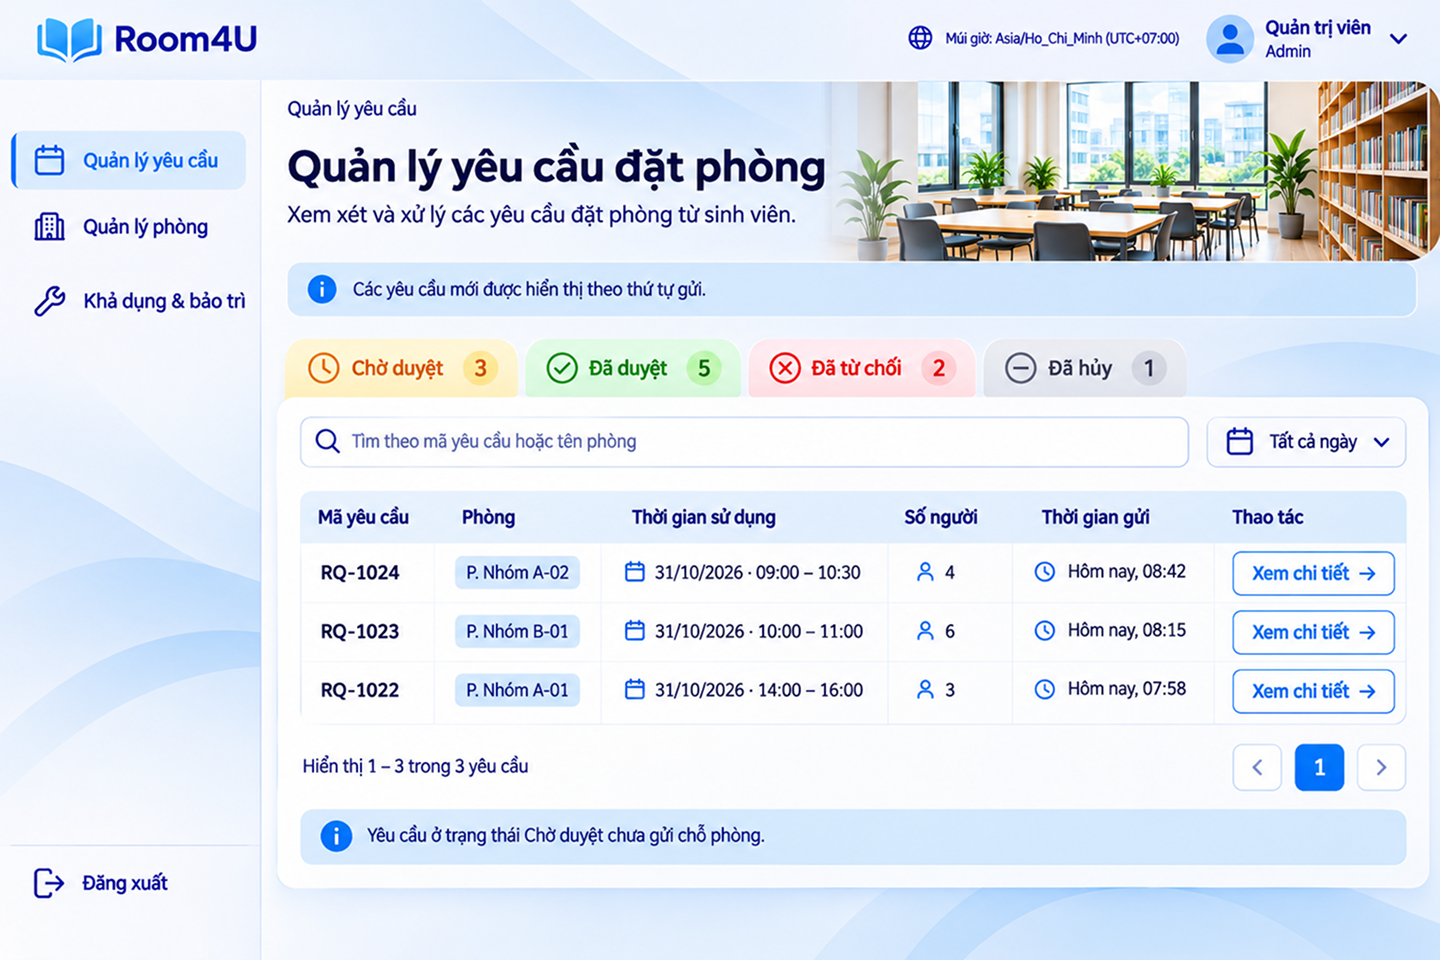
\includegraphics[width=0.9\textwidth,height=0.72\textheight,keepaspectratio]{images/image9.png}
\end{center}

\subsection*{9.2.2.2. S06 - Booking Request Details and
Processing}\label{s06---booking-request-details-and-processing}
\addcontentsline{toc}{subsection}{9.2.2.2. S06 - Booking Request Details
and Processing}

\begin{itemize}
\item
  Description: This screen presents the details and processing controls
  for a selected booking request. Its layout changes according to the
  request status. Common information includes booking details, requester
  information, room information, the room schedule, and
  request-processing history.

  \begin{itemize}
  \item
    Pending Requests: Administrators review the requested date and time,
    duration, number of participants, purpose, notes, requester details,
    room capacity, equipment, and room availability. They can approve a
    request when the slot is valid or reject it by providing a reason.
    Before approval, the system checks for scheduling conflicts. If the
    requested period is no longer available, the interface displays a
    conflict message and does not approve the request.
  \item
    Approved, Rejected, and Cancelled Requests: Administrators can
    review the booking information, current status, processing reason
    when applicable, and request history. For an Approved request, the
    detail screen provides a Cancel Booking action when cancellation is
    permitted. The administrator must enter a reason and confirm the
    action. The cancellation-reason field allows 1--250 characters after
    leading and trailing whitespace are removed (BR-13). Rejected and
    Cancelled requests are presented for review rather than as pending
    requests awaiting approval.
  \end{itemize}
\item
  \textbf{Mockup Views:}
\end{itemize}

\subsubsection{S06.1 -- Pending Request
Details:}\label{s06.1-pending-request-details}

\begin{quote}
\begin{center}
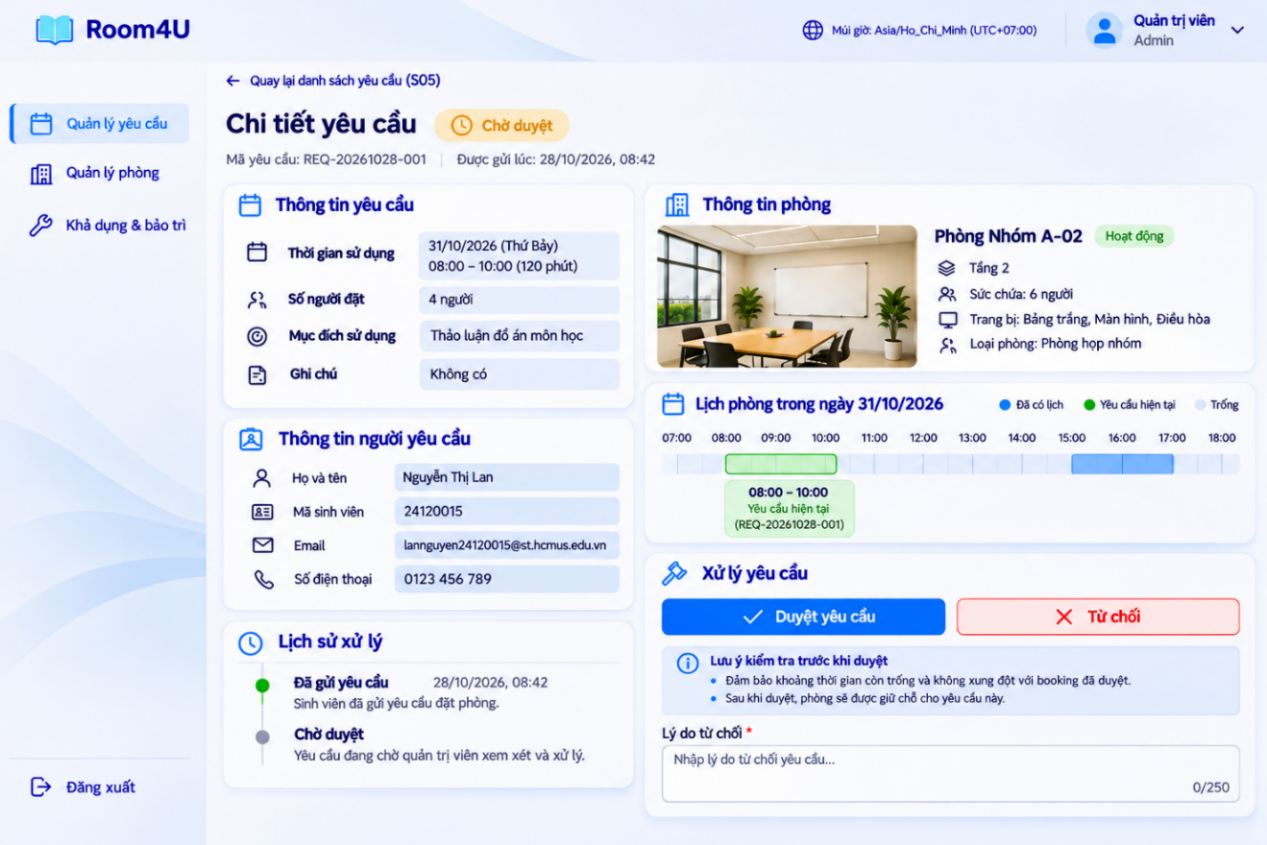
\includegraphics[width=0.9\textwidth,height=0.72\textheight,keepaspectratio]{images/image10.png}
\end{center}
\end{quote}

\subsubsection*{\texorpdfstring{ S06.1a -- Confirm
Approval:}{ S06.1a -- Confirm Approval:}}\label{s06.1a-confirm-approval}
\addcontentsline{toc}{subsubsection}{ S06.1a -- Confirm Approval:}

\begin{quote}
\begin{center}
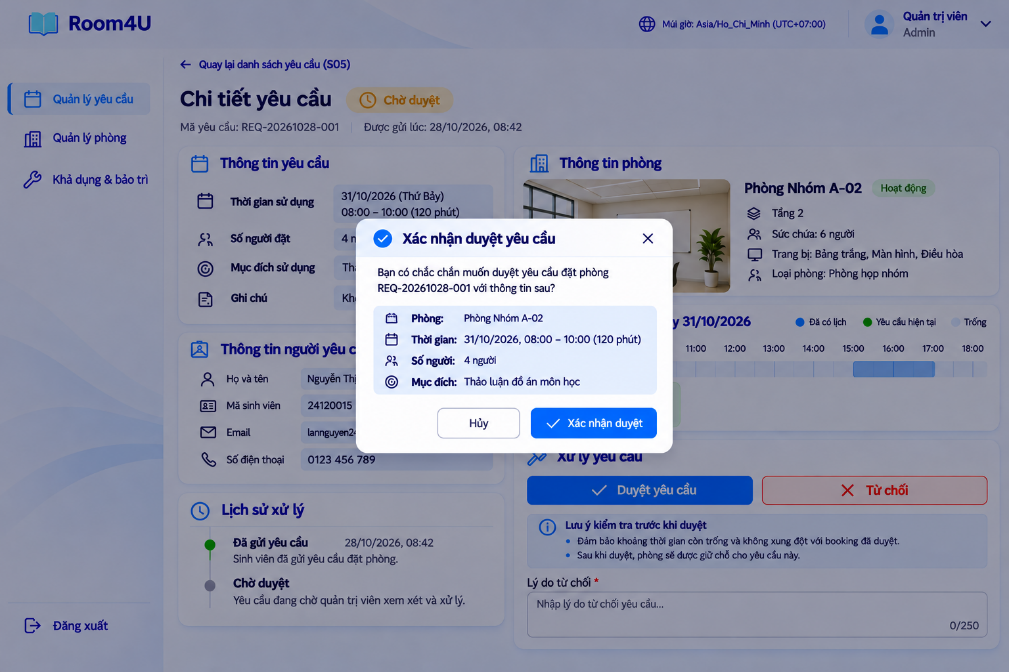
\includegraphics[width=0.9\textwidth,height=0.72\textheight,keepaspectratio]{images/image11.png}
\end{center}
\end{quote}

\subsubsection*{S06.1b -- Reject Request:}\label{s06.1b-reject-request}
\addcontentsline{toc}{subsubsection}{S06.1b -- Reject Request:}

\begin{quote}
\begin{center}
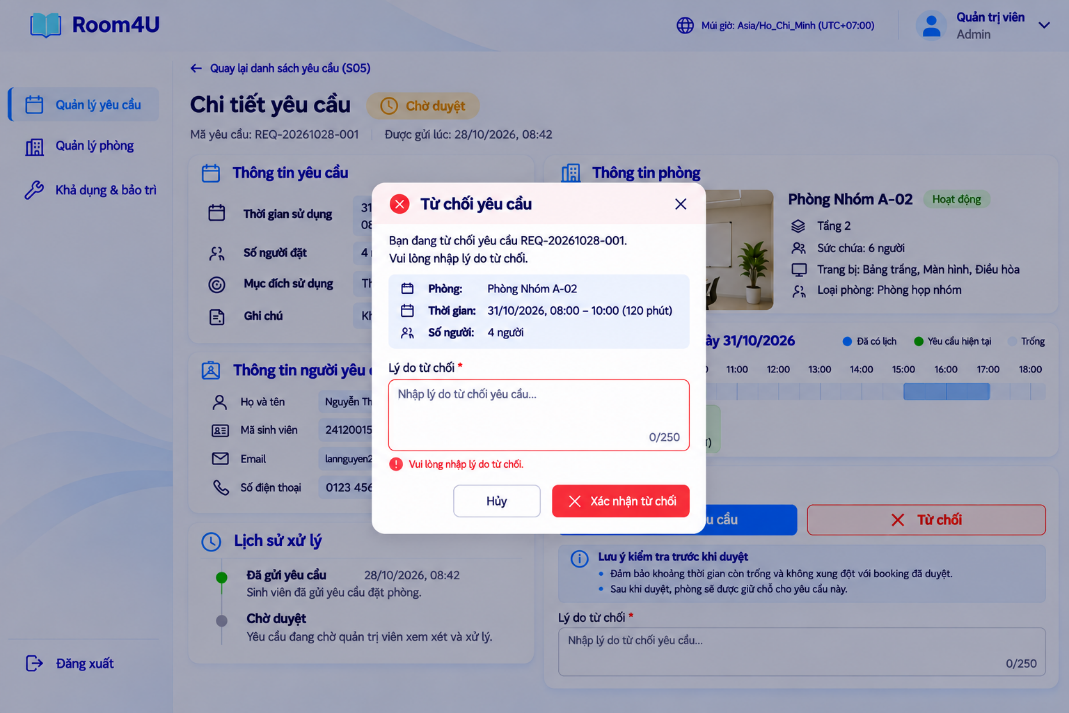
\includegraphics[width=0.9\textwidth,height=0.72\textheight,keepaspectratio]{images/image12.png}
\end{center}
\end{quote}

\subsubsection*{S06.1c -- Approval
Success:}\label{s06.1c-approval-success}
\addcontentsline{toc}{subsubsection}{S06.1c -- Approval Success:}

\begin{quote}
\begin{center}
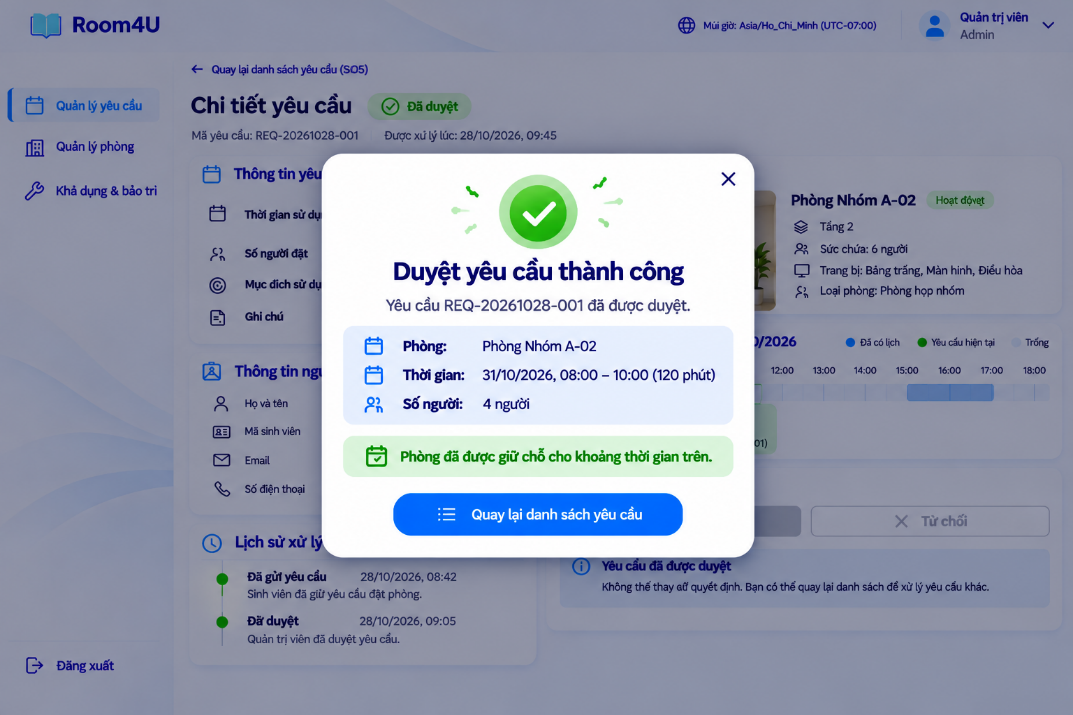
\includegraphics[width=0.9\textwidth,height=0.72\textheight,keepaspectratio]{images/image13.png}
\end{center}
\end{quote}

\subsubsection*{S06.1d -- Rejection
Success:}\label{s06.1d-rejection-success}
\addcontentsline{toc}{subsubsection}{S06.1d -- Rejection Success:}

\begin{quote}
\begin{center}
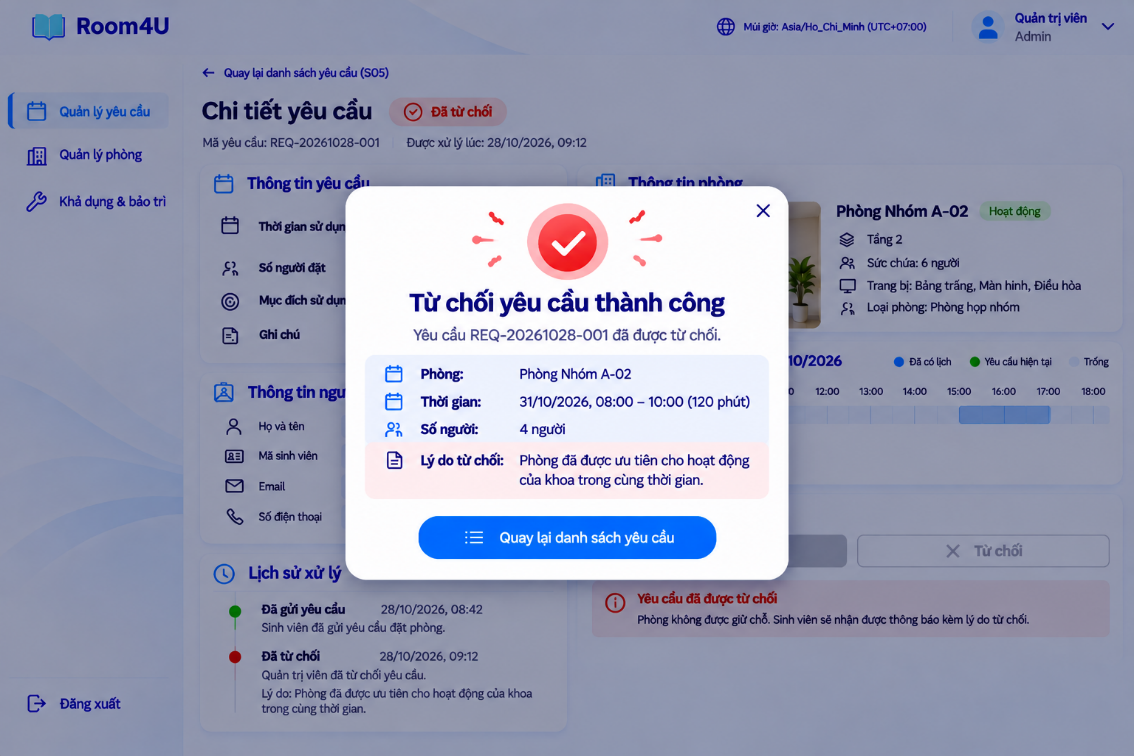
\includegraphics[width=0.9\textwidth,height=0.72\textheight,keepaspectratio]{images/image14.png}
\end{center}
\end{quote}

\subsubsection*{S06.1e -- Scheduling
Conflict:}\label{s06.1e-scheduling-conflict}
\addcontentsline{toc}{subsubsection}{S06.1e -- Scheduling Conflict:}

\begin{quote}
\begin{center}
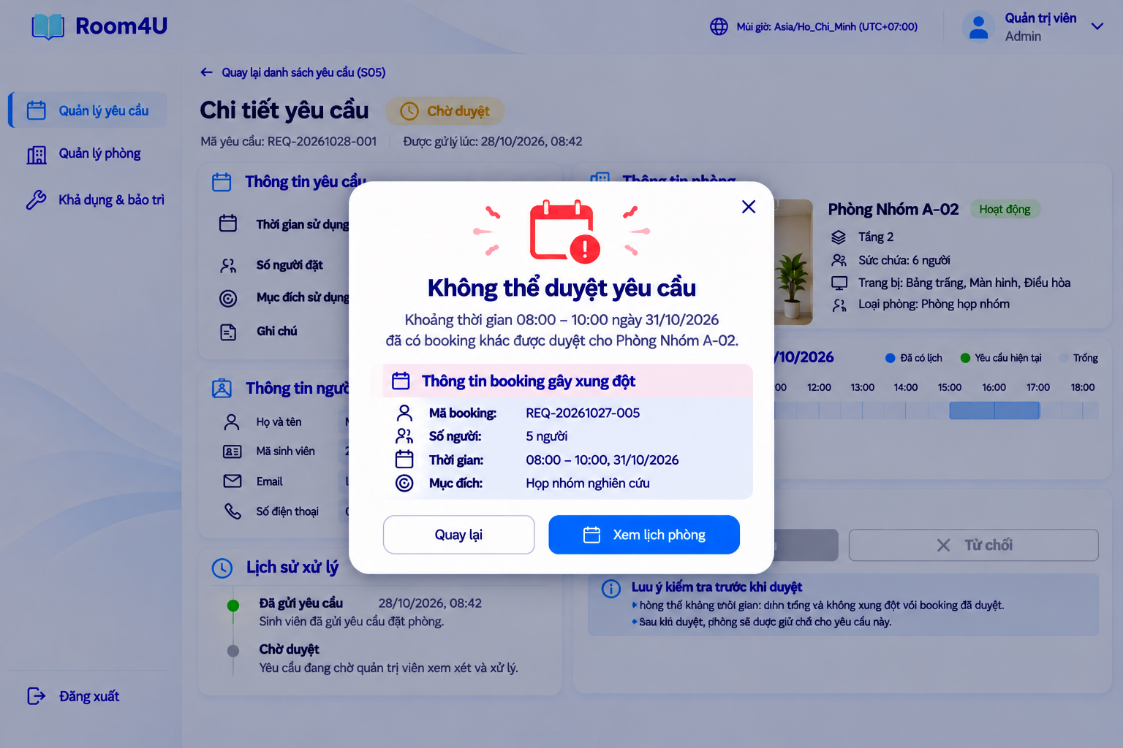
\includegraphics[width=0.9\textwidth,height=0.72\textheight,keepaspectratio]{images/image15.png}
\end{center}
\end{quote}

\subsubsection{S06.2 -- Approved Request Details and
Cancellation:}\label{s06.2-approved-request-details-and-cancellation}

\begin{quote}
\begin{center}
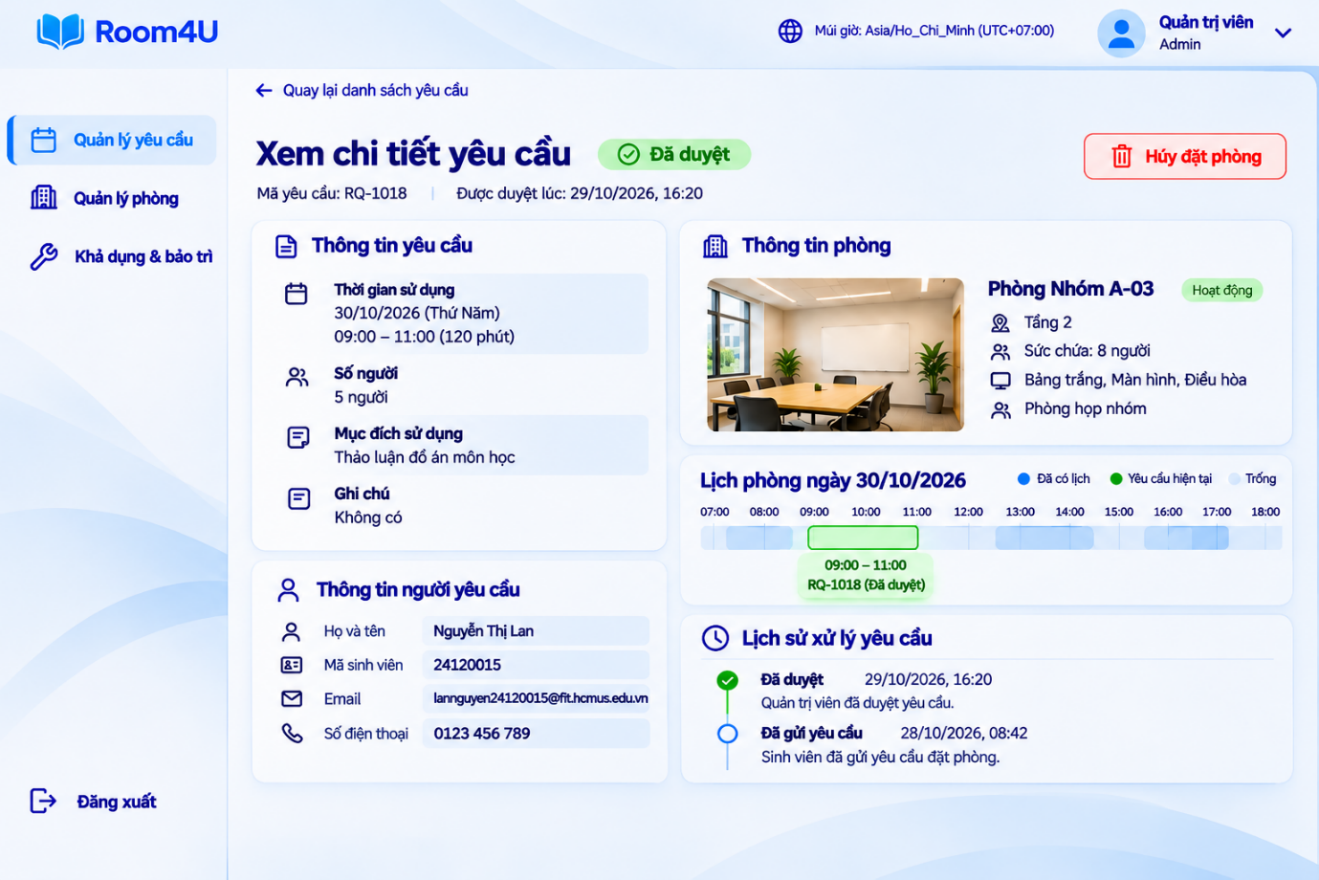
\includegraphics[width=0.9\textwidth,height=0.72\textheight,keepaspectratio]{images/image16.png}
\end{center}

\begin{center}
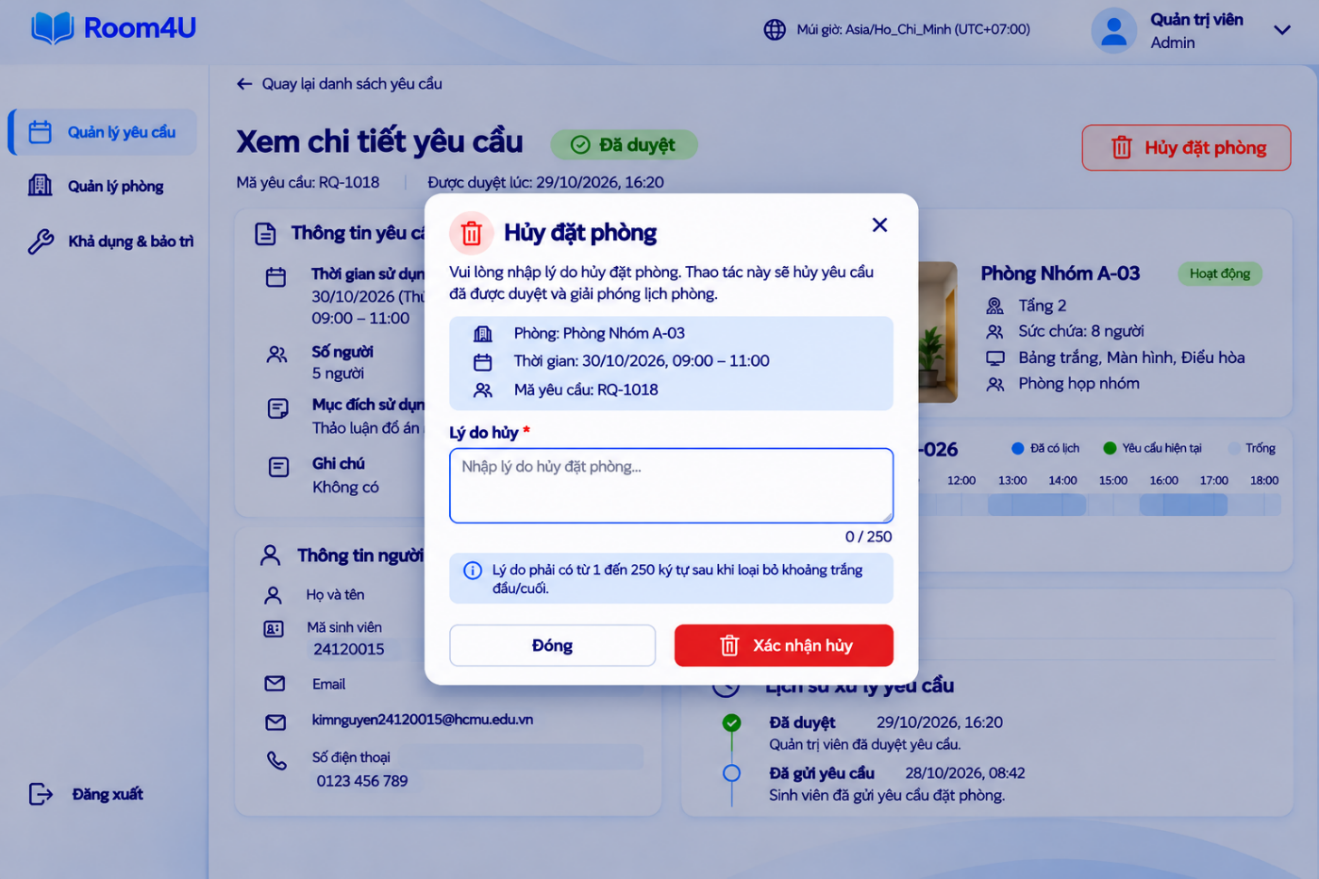
\includegraphics[width=0.9\textwidth,height=0.72\textheight,keepaspectratio]{images/image17.png}
\end{center}

\begin{center}
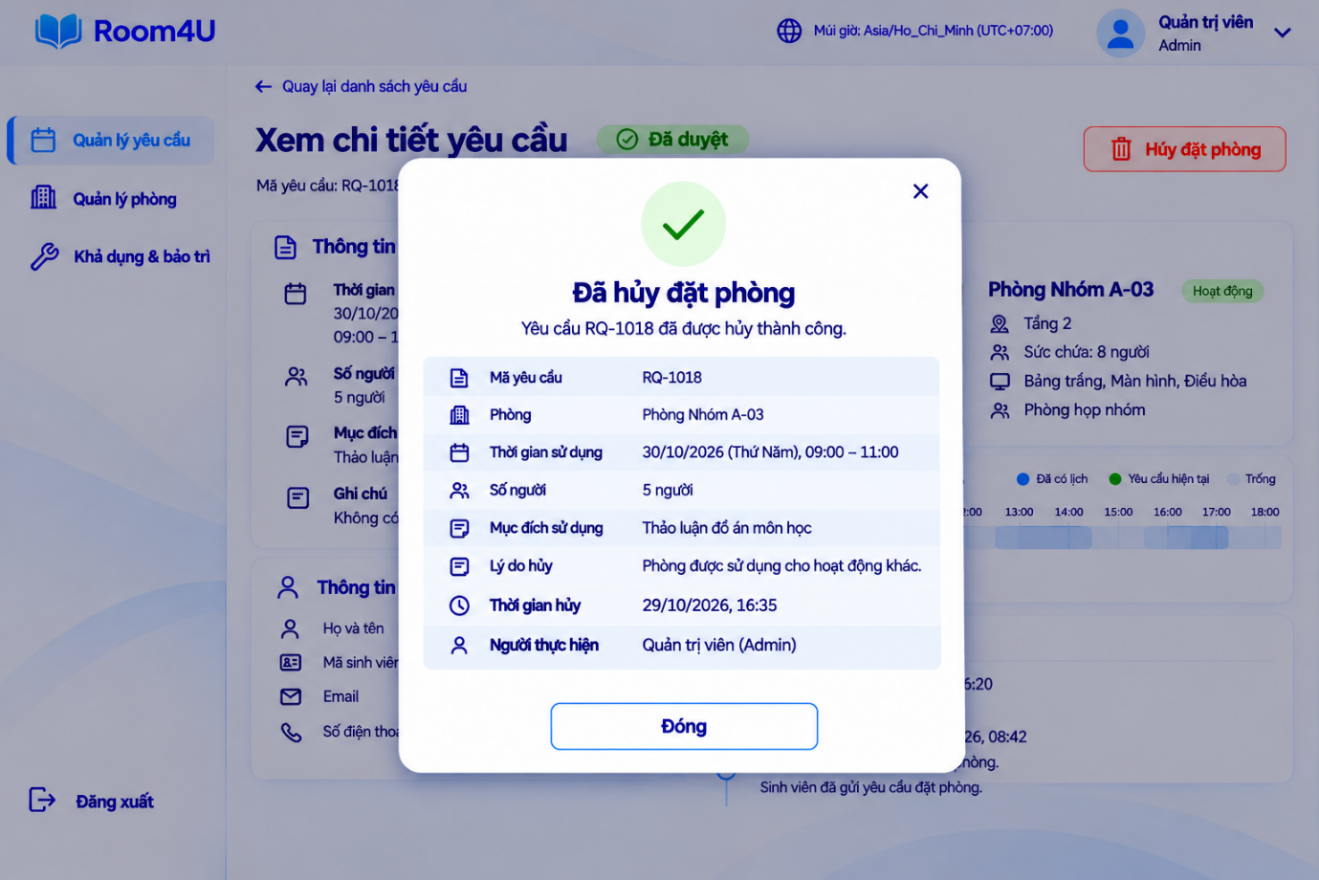
\includegraphics[width=0.9\textwidth,height=0.72\textheight,keepaspectratio]{images/image18.png}
\end{center}
\end{quote}

Approved Booking Cancellation: The administrator can initiate
cancellation from the Approved Request Details screen when the
applicable conditions allow it. A cancellation dialog requests a reason
and asks the administrator to confirm. The reason must contain 1--250
characters after trimming leading and trailing whitespace (BR-13). After
confirmation, the request is updated to Cancelled and the interface
displays the result and relevant booking information.

\subsubsection{S06.3 -- Rejected Request
Details:}\label{s06.3-rejected-request-details}

\begin{quote}
\begin{center}
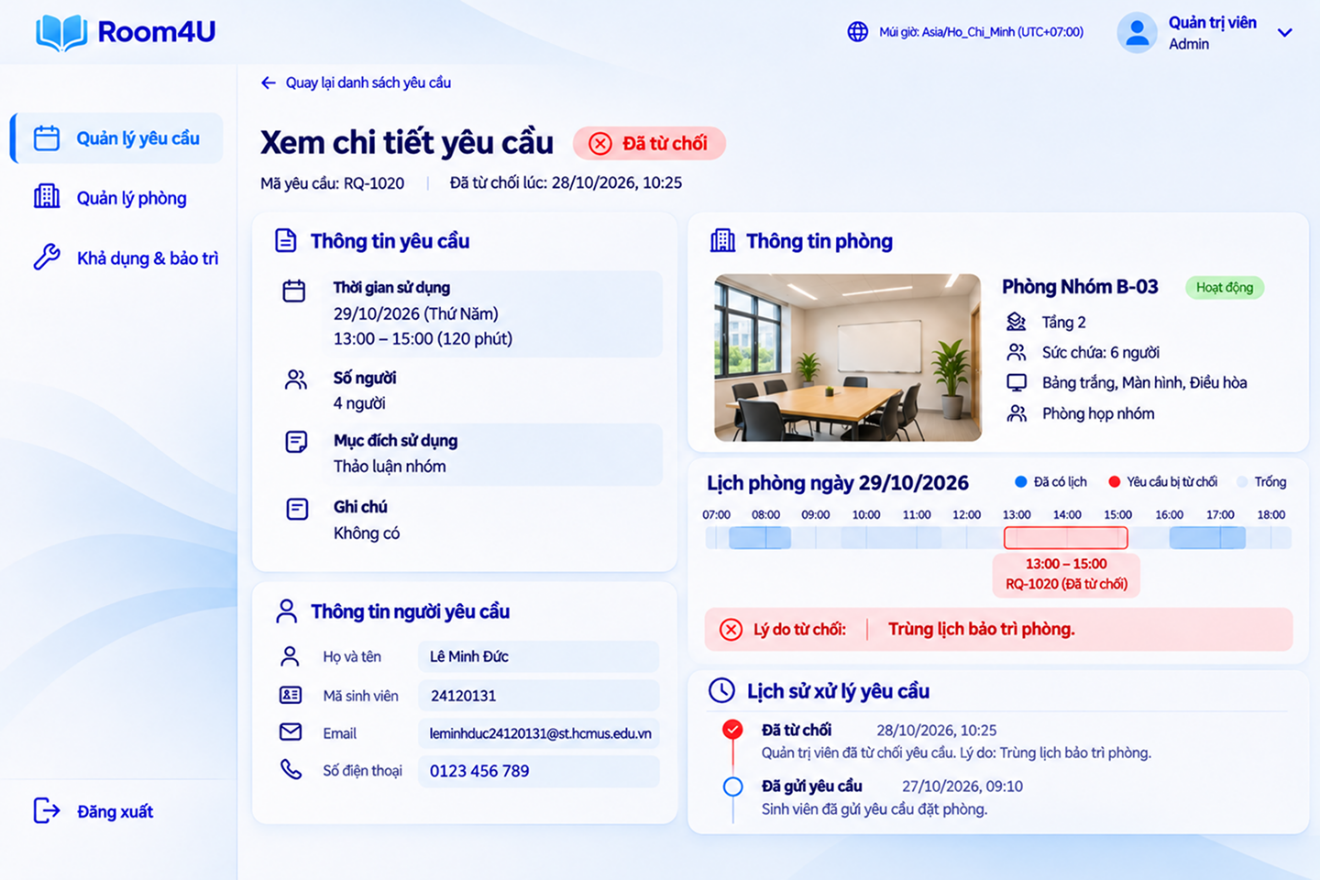
\includegraphics[width=0.9\textwidth,height=0.72\textheight,keepaspectratio]{images/image19.png}
\end{center}
\end{quote}

\subsubsection{S06.4 -- Cancelled Request
Details:}\label{s06.4-cancelled-request-details}

\begin{quote}
\begin{center}
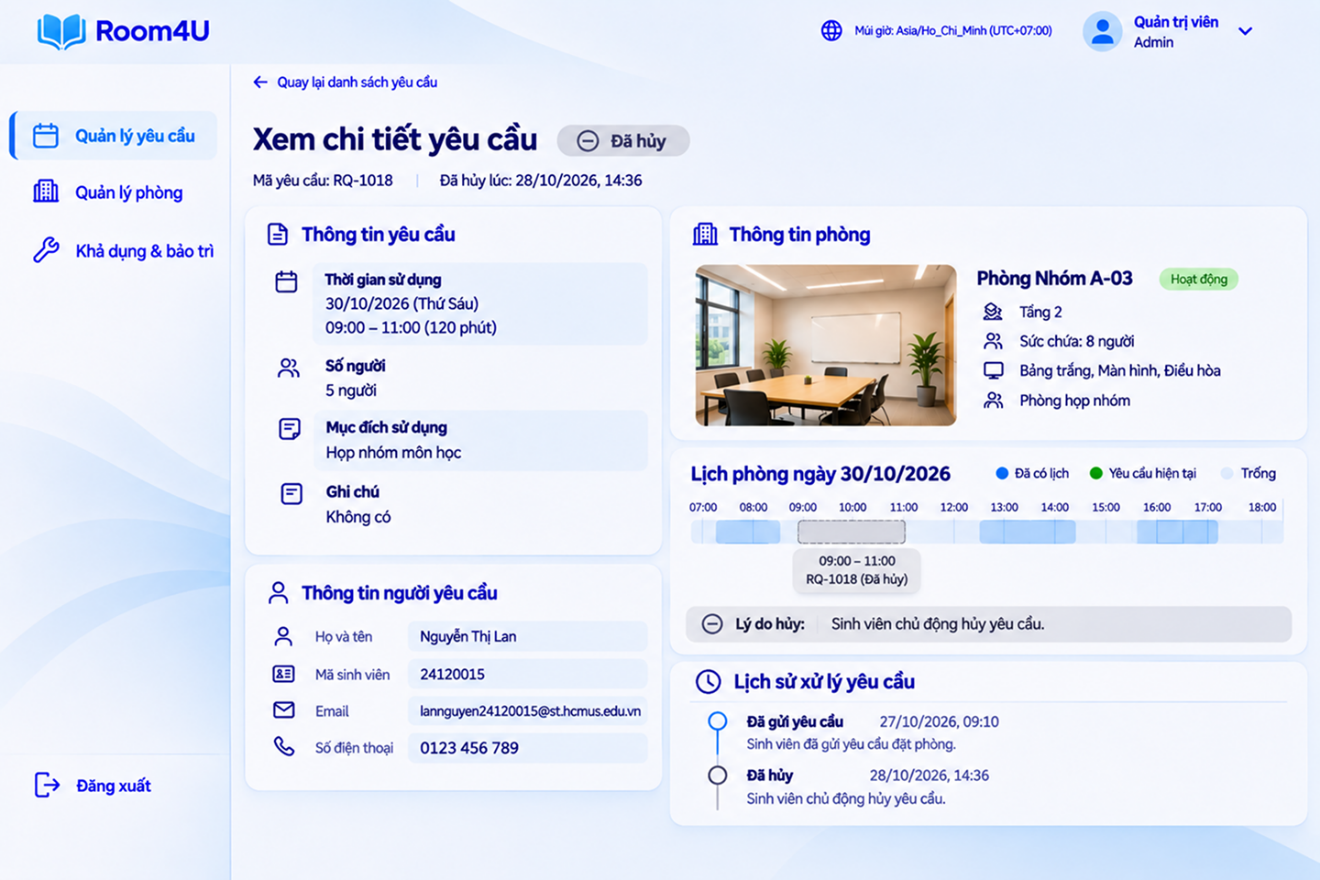
\includegraphics[width=0.9\textwidth,height=0.72\textheight,keepaspectratio]{images/image20.png}
\end{center}
\end{quote}

\subsection*{9.2.2.3. S07 - Room
Management}\label{s07---room-management}
\addcontentsline{toc}{subsection}{9.2.2.3. S07 - Room Management}

\begin{itemize}
\item
  Description: This screen allows administrators to manage room records
  and monitor each room's current status. Summary cards
  show the total number of rooms and the counts of Active, Under
  Maintenance, and Suspended rooms. Administrators can search for a room
  and filter the list by floor or status. The room table and detail
  panel show the room code, room name, floor, capacity, equipment,
  description, and status. Available actions include adding a room,
  editing room information, and suspending or resuming a room, subject
  to the system rules.
\item
  \textbf{Mockup View:}
  \begin{center}
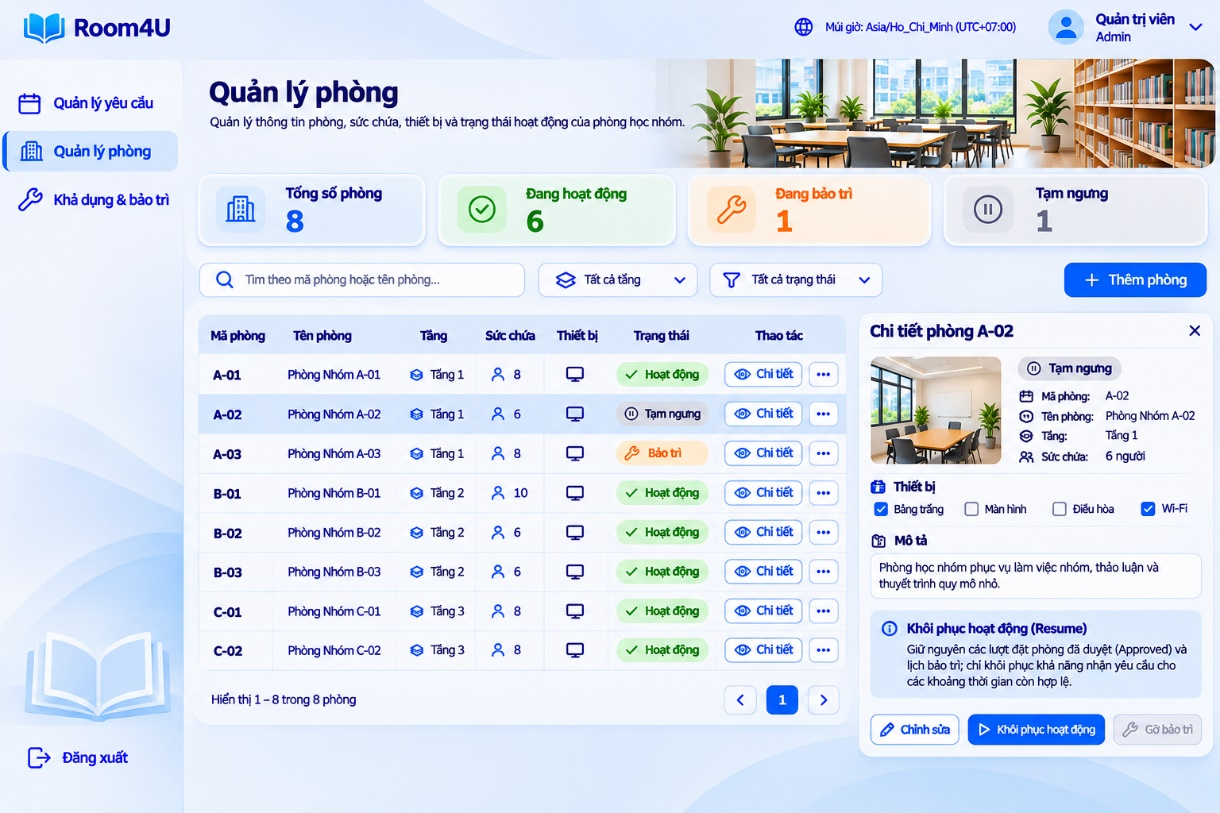
\includegraphics[width=0.9\textwidth,height=0.72\textheight,keepaspectratio]{images/image21.jpeg}
\end{center}
\end{itemize}

Room Creation: The Add Room dialog collects a unique room code, room
name, floor, capacity, equipment selections, and an optional
description. The room code must be unique without case sensitivity after
leading and trailing whitespace are removed. Capacity must be an integer
from 1 to 50. The description is optional and limited to 250 characters.
After a valid submission, a success dialog confirms that the new room
has been added and shows its key details.

Room Editing: The Edit Room dialog displays the selected room's existing
information for update. Administrators can update the room code, name,
floor, capacity, equipment, and optional description. The internal room
ID remains unchanged. The room code may be updated subject to the
uniqueness rules in BR-14. When Save is selected, Room4U revalidates the
fields, including room-code uniqueness, and checks the proposed capacity
against current future Approved bookings. The save is consistent with
concurrent approvals so no future Approved booking can exceed the saved
room capacity. After a valid update, a success dialog confirms that the
room information has been updated.

Suspend and Resume: The room detail panel provides the applicable
room-status action. When a suspended room is resumed, existing Approved
bookings and maintenance schedules are preserved. Resume restores the
ability to receive new booking requests only for time periods that
remain valid; it does not cancel, modify, or overwrite existing bookings
or maintenance records.

\subsection*{9.2.2.4. S08 - Room Availability and
Maintenance}\label{s08---room-availability-and-maintenance}
\addcontentsline{toc}{subsection}{9.2.2.4. S08 - Room Availability and
Maintenance}

\begin{itemize}
\item
  Description: This screen allows administrators to inspect room usage
  and manage maintenance schedules. The interface separates the
  room-usage calendar from the maintenance schedule so that Approved
  bookings and maintenance records can be reviewed without confusing
  their meanings.

  \begin{itemize}
  \item
    Room Usage History: Administrators can inspect room schedules in the
    available calendar views and identify Approved bookings, maintenance
    periods, and available time slots. The schedule is organized by room
    and date to support availability checks.
  \item
    Maintenance Schedule: Administrators can view existing maintenance
    records, create a maintenance schedule, inspect its details, and
    remove its effect when eligible. A maintenance record identifies the
    affected room, start and end time, reason, and status. The
    maintenance list provides view and remove actions; an edit action is
    not included in the current UC-13 flow.
  \item
    Maintenance Rules and Removal Flow: To create a maintenance
    schedule, the administrator specifies the room, start time, end
    time, and reason. The system rejects creation if the requested
    period overlaps an Approved booking or an active maintenance period.
    Creating maintenance does not automatically cancel or modify an
    Approved booking. To remove a schedule's effect, the
    administrator selects a block that is Active and has not started,
    reviews the information, and confirms the action. On success, the
    system removes the block' s effect on availability,
    updates the room schedule, and retains the maintenance record for
    reference. If the block has already started or no longer meets the
    eligibility conditions, the system displays an error and makes no
    change to the record.
  \end{itemize}
\item
  \textbf{Mockup Views:}

  \begin{itemize}
  \item
    \textbf{S08.1 -- Room Usage History:}
  \end{itemize}
\end{itemize}

\begin{quote}
\begin{center}
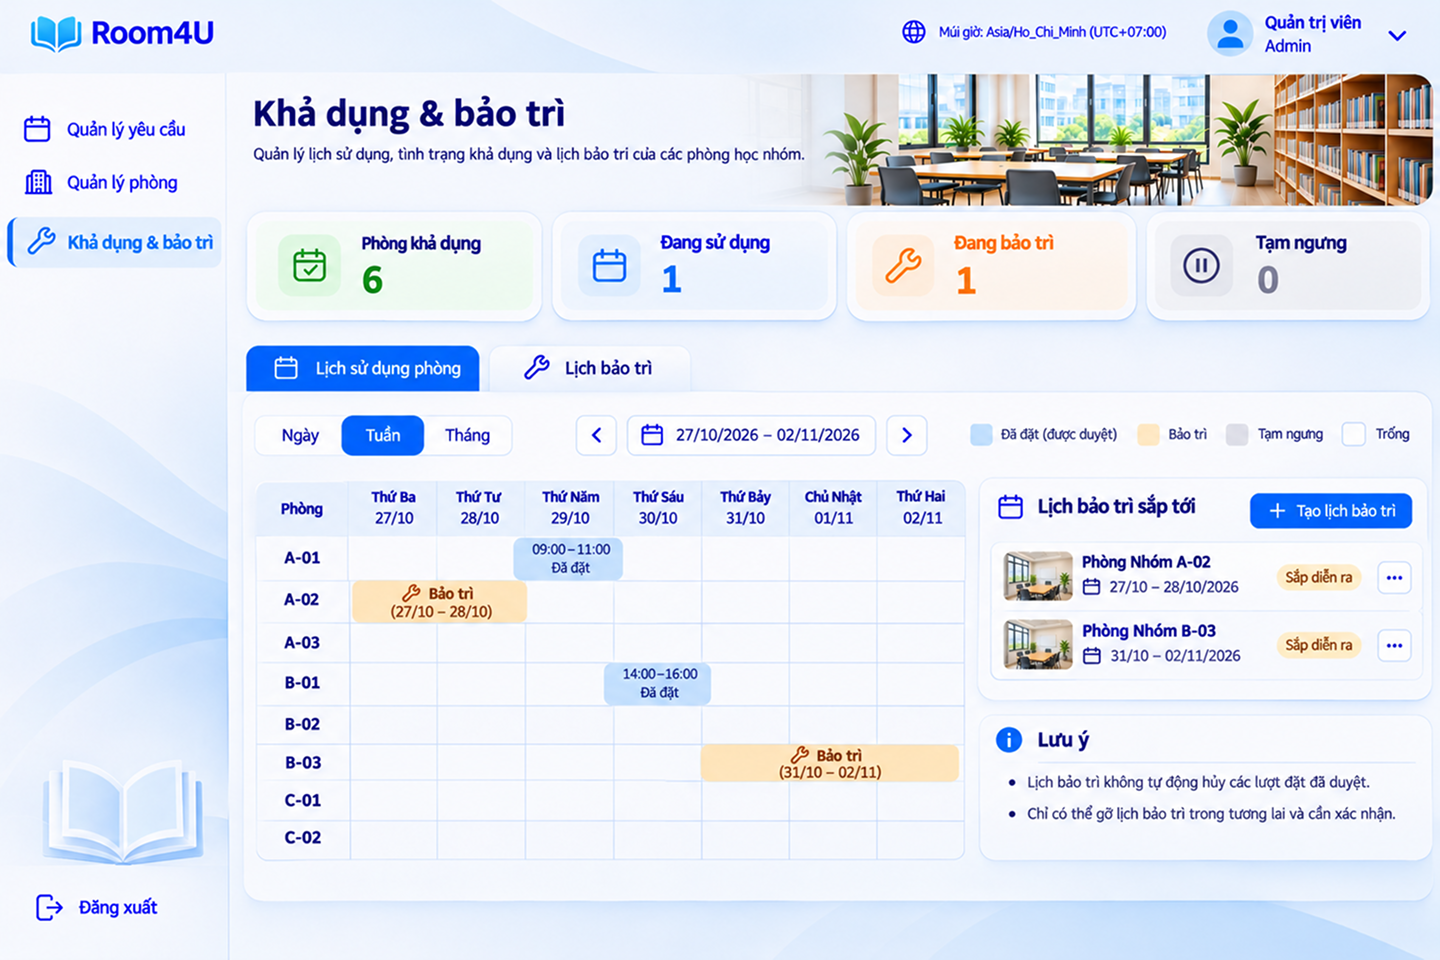
\includegraphics[width=0.9\textwidth,height=0.72\textheight,keepaspectratio]{images/image22.png}
\end{center}
\end{quote}

Create Maintenance Schedule: The creation dialog collects the room,
maintenance date, start time, end time, and reason. The end time must be
later than the start time. The system validates the selected interval
against Approved bookings and active maintenance schedules before
creating the record.

Maintenance List Actions: Each maintenance record can be viewed or
selected for removal when eligible. The current flow does not provide an
edit action. A successful removal deactivates the
schedule's effect but retains its record; unsuccessful
removal leaves the record and schedule unchanged.

\begin{itemize}
\item
  \textbf{S08.2 -- Maintenance Schedule:}
\end{itemize}

\begin{quote}
\begin{center}
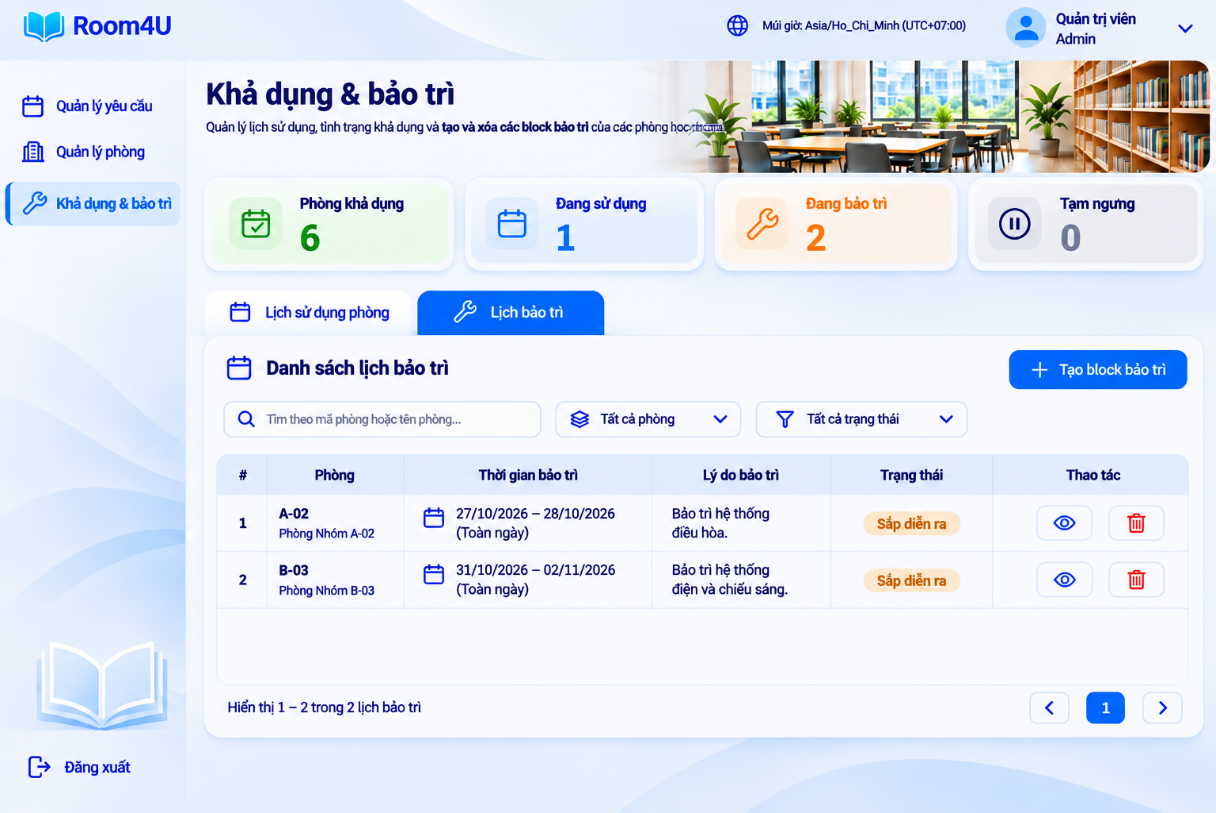
\includegraphics[width=0.9\textwidth,height=0.72\textheight,keepaspectratio]{images/image23.png}
\end{center}

\textbf{Case 1 -- Removal Not Allowed:} The maintenance schedule has
already started. The system explains that the schedule is no longer
eligible for removal, provides the room and schedule details, and offers
a Close action. The record and its effect remain unchanged.

\begin{center}
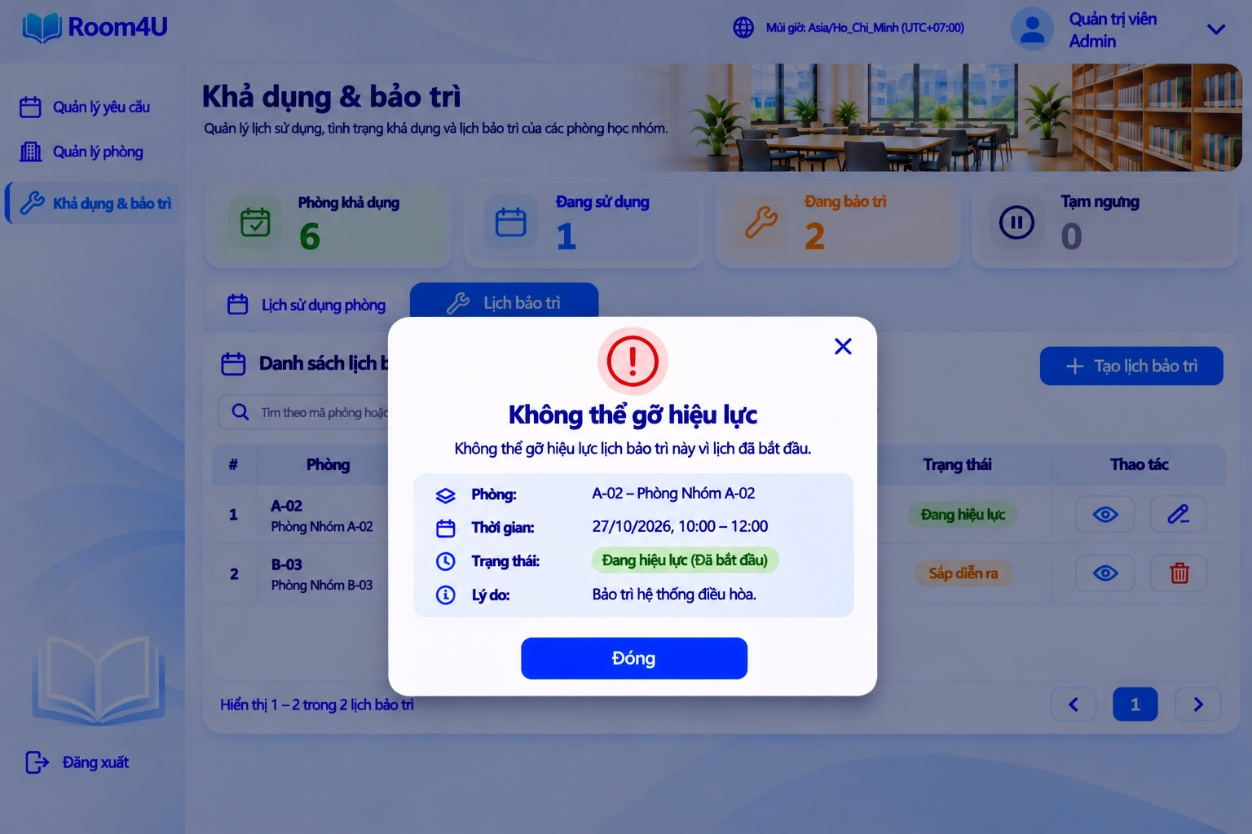
\includegraphics[width=0.9\textwidth,height=0.72\textheight,keepaspectratio]{images/image24.jpeg}
\end{center}

\textbf{Case 2 -- Creation Not Allowed --- Conflicting Approved
Booking:} The system rejects the creation because the requested
maintenance period overlaps with an existing Approved booking (FR-25).
The dialog displays the affected room and conflicting time periods. No
new maintenance record is created, and existing bookings remain
unchanged.

\begin{center}
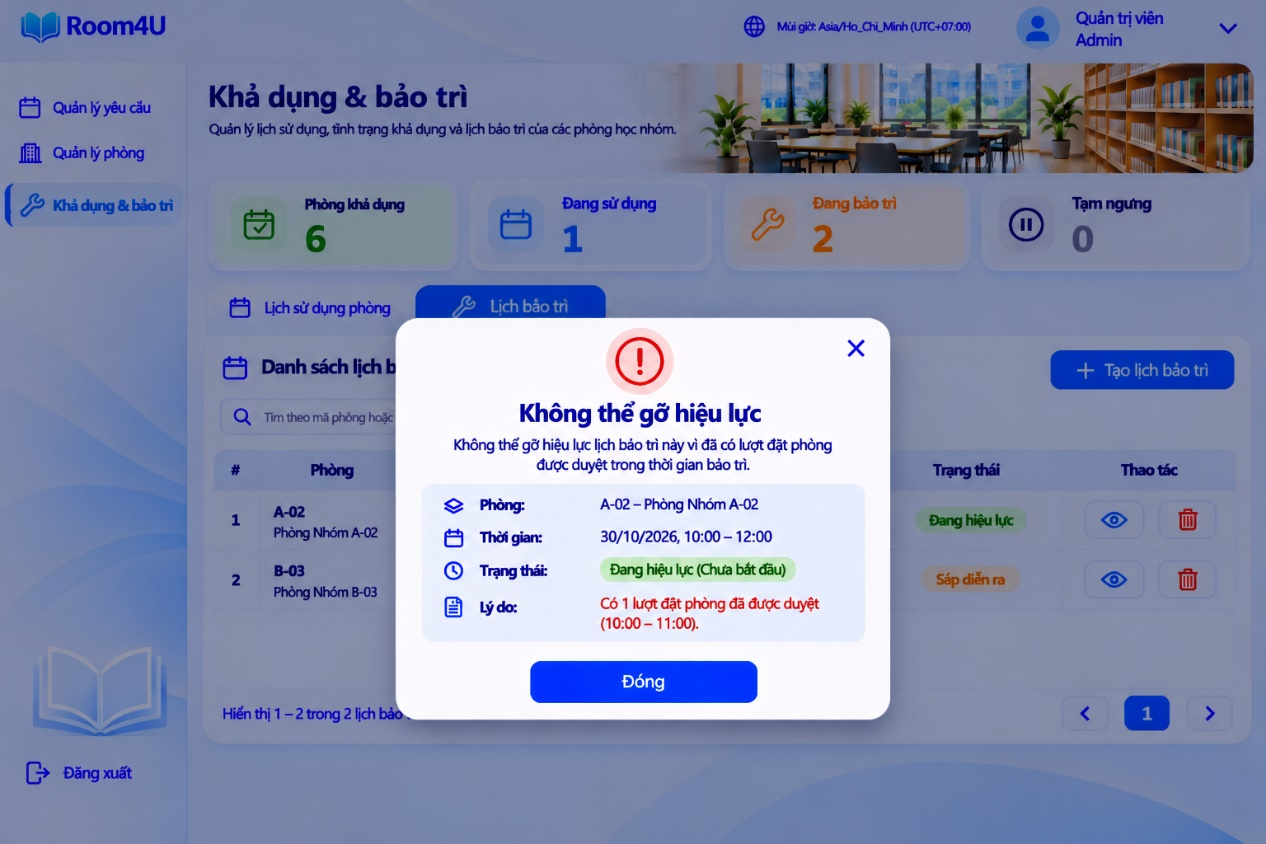
\includegraphics[width=0.9\textwidth,height=0.72\textheight,keepaspectratio]{images/image25.jpeg}
\end{center}
\end{quote}

\section*{9.3. Accessibility
Considerations}\label{accessibility-considerations}
\addcontentsline{toc}{section}{9.3. Accessibility Considerations}

Color and Status Indicators: The blue-and-white palette maintains a
consistent visual hierarchy. Statuses use distinct text labels and
supporting icons as well as color, so meaning is not communicated by
color alone.

Input Labels and Feedback: Form fields use visible labels and helpful
placeholders. Required fields and validation messages should be clearly
identified, especially for booking submission, rejection reasons, room
creation and editing, and administrator cancellation reasons.

\begin{itemize}
\item
  Keyboard and Focus: Interactive controls such as buttons, search
  fields, form inputs, navigation items, and dialogs should have a
  logical keyboard order and a visible focus state during
  implementation.
\item
  Keyboard Navigation: Interactive elements, including buttons, input
  fields, dropdowns, and navigation links, should support keyboard
  navigation to improve accessibility and usability.
\item
  Dialog Feedback: Confirmation, success, and error dialogs should have
  clear titles, concise explanations, and action labels that describe
  the outcome. Error dialogs should explain why an operation is blocked
  and confirm that the underlying record remains unchanged.
\end{itemize}

\section{Requirements Traceability Matrix}

Every functional requirement (FR), non-functional requirement (NFR) and business rule (BR) below is traced to related use cases and screens where directly applicable, a planned PA3 design topic and a planned PA4 verification reference. System-wide operational requirements may use N/A where there is no direct user-facing use case or screen. The design topics and verification references are plans, not completed artifacts. PA3 will replace the planned topics with actual diagram or component references; PA4 will replace acceptance criteria and verification methods with concrete test-case identifiers.

FR-02, FR-03 and NFR-02 are cross-cutting constraints for every protected operation in UC-03--UC-13, including Student operations UC-04--UC-06. UC-14 inherits the caller's identity, role and ownership checks from UC-04 or UC-08 and has no independent actor or screen. UC-01 is sign-in; UC-02 can clear local private data when its session has expired. In grouped mappings, UC-12 uses S07 for Suspend/Resume, while S08 maps maintenance operations to UC-13.

\subsection{Functional Requirements}
\begingroup
\small
\setstretch{1.0}
\setlength{\tabcolsep}{3pt}
\renewcommand{\arraystretch}{1.1}
\begin{longtable}{|>{\raggedright\arraybackslash}p{0.085\textwidth}|>{\raggedright\arraybackslash}p{0.19\textwidth}|>{\raggedright\arraybackslash}p{0.13\textwidth}|>{\raggedright\arraybackslash}p{0.28\textwidth}|>{\raggedright\arraybackslash}p{0.225\textwidth}|}
\hline
\textbf{Req. ID} & \textbf{Related use cases} & \textbf{Related screens} & \textbf{Planned PA3 design topic} & \textbf{Planned PA4 verification} \\ \hline
\endfirsthead
\hline
\textbf{Req. ID} & \textbf{Related use cases} & \textbf{Related screens} & \textbf{Planned PA3 design topic} & \textbf{Planned PA4 verification} \\ \hline
\endhead
\hline
\endfoot
\hline
\endlastfoot
FR-01 & UC-01 & S01 & Identity and access design & AC-01 \\ \hline
FR-02 & UC-03--UC-13 (cross-cutting); UC-02 local-sign-out exception; UC-14 via caller & S02--S08 & Identity and access design & AC-02 \\ \hline
FR-03 & UC-01, UC-03--UC-13 (cross-cutting); UC-14 via caller & S01--S08 & Identity and access design & AC-02 \\ \hline
FR-04 & UC-05, UC-06 & S04 & Identity and access design & AC-02 \\ \hline
FR-05 & UC-02 & S02--S08 & Identity and access design & AC-03 \\ \hline
FR-06 & UC-03 & S02 & Room queries and calendar & AC-04 \\ \hline
FR-07 & UC-03 & S02 & Room queries and calendar & AC-04 \\ \hline
FR-08 & UC-03 & S02 & Room queries and calendar & AC-05 \\ \hline
FR-09 & UC-03 & S02 & Room queries and calendar & AC-05 \\ \hline
FR-10 & UC-04, UC-14 & S03 & Request lifecycle & AC-06, AC-07 \\ \hline
FR-11 & UC-04 & S03, S04 & Request lifecycle & AC-06 \\ \hline
FR-12 & UC-05 & S04 & Request lifecycle & AC-08 \\ \hline
FR-13 & UC-06 & S04 & Request lifecycle & AC-09 \\ \hline
FR-14 & UC-07 & S05, S06 & Approval transaction and history & AC-10 \\ \hline
FR-15 & UC-08, UC-14 & S06 & Approval transaction and history & AC-10, AC-11 \\ \hline
FR-16 & UC-08 (S06), UC-12 (S07), UC-13 (S08) & S06, S07, S08 & Approval transaction and history & AC-11, AC-12 \\ \hline
FR-17 & UC-09 & S06, S04 & Approval transaction and history & AC-13 \\ \hline
FR-18 & UC-10 & S06, S04 & Approval transaction and history & AC-14 \\ \hline
FR-19 & UC-04, UC-06, UC-08--UC-10 & S04, S06 & Approval transaction and history & AC-08, AC-14 \\ \hline
FR-20 & UC-11 & S07 & Room and maintenance design & AC-15 \\ \hline
FR-21 & UC-11 & S07 & Room and maintenance design & AC-15 \\ \hline
FR-22 & UC-12 & S07 & Room and maintenance design & AC-16 \\ \hline
FR-23 & UC-12 & S07 & Room and maintenance design & AC-16 \\ \hline
FR-24 & UC-13 & S08 & Room and maintenance design & AC-17 \\ \hline
FR-25 & UC-13 & S08, S06 & Room and maintenance design & AC-12, AC-17 \\ \hline
FR-26 & UC-13 & S08 & Room and maintenance design & AC-18 \\ \hline
FR-27 & UC-03 (S02), UC-11--UC-12 (S07), UC-13 (S08) & S02, S07, S08 & Room and maintenance design & AC-16--AC-18 \\ \hline
\end{longtable}
\endgroup

\subsection{Non-Functional Requirements}
\begingroup
\small
\setstretch{1.0}
\setlength{\tabcolsep}{3pt}
\renewcommand{\arraystretch}{1.1}
\begin{longtable}{|>{\raggedright\arraybackslash}p{0.085\textwidth}|>{\raggedright\arraybackslash}p{0.19\textwidth}|>{\raggedright\arraybackslash}p{0.13\textwidth}|>{\raggedright\arraybackslash}p{0.28\textwidth}|>{\raggedright\arraybackslash}p{0.225\textwidth}|}
\hline
\textbf{Req. ID} & \textbf{Related use cases} & \textbf{Related screens} & \textbf{Planned PA3 design topic} & \textbf{Planned PA4 verification} \\ \hline
\endfirsthead
\hline
\textbf{Req. ID} & \textbf{Related use cases} & \textbf{Related screens} & \textbf{Planned PA3 design topic} & \textbf{Planned PA4 verification} \\ \hline
\endhead
\hline
\endfoot
\hline
\endlastfoot
NFR-01 & UC-03, UC-05 & S02, S04 & Quality and cross-cutting design & NFR-01 verification method in Section 6.2 \\ \hline
NFR-02 & UC-03--UC-13 (cross-cutting); UC-02 local-sign-out exception; UC-14 via caller & S02--S08 & Quality and cross-cutting design & NFR-02 verification method in Section 6.2 \\ \hline
NFR-03 & UC-08 (S06), UC-12 (S07), UC-13 (S08) & S06, S07, S08 & Quality and cross-cutting design & NFR-03 verification method in Section 6.2 \\ \hline
NFR-04 & UC-01, UC-03--UC-06, UC-08 & S01--S08 & Quality and cross-cutting design & NFR-04 verification method in Section 6.2 \\ \hline
NFR-05 & UC-03--UC-05 & S02--S04 & Quality and cross-cutting design & NFR-05 verification method in Section 6.2 \\ \hline
NFR-06 & UC-01--UC-13 & All screens & Quality and cross-cutting design & NFR-06 verification method in Section 6.2 \\ \hline
NFR-07 & UC-01--UC-13 & S01--S08 & Quality and cross-cutting design & NFR-07 verification method in Section 6.2 \\ \hline
NFR-08 & N/A -- system-wide operational requirement & N/A -- no direct user-facing screen & Backup and recovery planning & NFR-08 restore drill in Section 6.2 \\ \hline
NFR-09 & UC-04, UC-06, UC-08--UC-13 & S03--S08 & Quality and cross-cutting design & NFR-09 verification method in Section 6.2 \\ \hline
NFR-10 & UC-04--UC-06, UC-08--UC-10 & S04, S06 & Quality and cross-cutting design & NFR-10 verification method in Section 6.2 \\ \hline
NFR-11 & UC-04, UC-08--UC-13 & S03, S06--S08 & Quality and cross-cutting design & NFR-11 verification method in Section 6.2 \\ \hline
NFR-12 & UC-01--UC-13 & S01--S08 & Quality and cross-cutting design & NFR-12 verification method in Section 6.2 \\ \hline
\end{longtable}
\endgroup

\subsection{Business Rules}
\begingroup
\small
\setstretch{1.0}
\setlength{\tabcolsep}{3pt}
\renewcommand{\arraystretch}{1.1}
\begin{longtable}{|>{\raggedright\arraybackslash}p{0.085\textwidth}|>{\raggedright\arraybackslash}p{0.19\textwidth}|>{\raggedright\arraybackslash}p{0.13\textwidth}|>{\raggedright\arraybackslash}p{0.28\textwidth}|>{\raggedright\arraybackslash}p{0.225\textwidth}|}
\hline
\textbf{Rule ID} & \textbf{Related use cases} & \textbf{Related screens} & \textbf{Planned PA3 design topic} & \textbf{Planned PA4 acceptance seeds} \\ \hline
\endfirsthead
\hline
\textbf{Rule ID} & \textbf{Related use cases} & \textbf{Related screens} & \textbf{Planned PA3 design topic} & \textbf{Planned PA4 acceptance seeds} \\ \hline
\endhead
\hline
\endfoot
\hline
\endlastfoot
BR-01 & UC-01, UC-04 & S01, S03 & Rule enforcement and state model & AC-01, AC-06 \\ \hline
BR-02 & UC-04, UC-08, UC-14 & S03, S06 & Rule enforcement and state model & AC-07 \\ \hline
BR-03 & UC-04, UC-08, UC-14 & S03, S06 & Rule enforcement and state model & AC-07 \\ \hline
BR-04 & UC-04, UC-08, UC-14 & S03, S06 & Rule enforcement and state model & AC-07, AC-11 \\ \hline
BR-05 & UC-03, UC-04, UC-08, UC-11, UC-14 & S02, S03, S06, S07 & Rule enforcement and state model & AC-04, AC-07, AC-15 \\ \hline
BR-06 & UC-03, UC-04, UC-08, UC-13, UC-14 & S02, S03, S06, S08 & Rule enforcement and state model & AC-07, AC-11, AC-17 \\ \hline
BR-07 & UC-03, UC-04, UC-08, UC-13 & S02, S03, S06, S08 & Rule enforcement and state model & AC-05, AC-06, AC-11 \\ \hline
BR-08 & UC-08, UC-13, UC-14 & S06, S08 & Rule enforcement and state model & AC-11, AC-12 \\ \hline
BR-09 & UC-04, UC-06, UC-08--UC-10 & S03, S04, S06 & Rule enforcement and state model & AC-06, AC-09--AC-14 \\ \hline
BR-10 & UC-06, UC-09, UC-10 & S04, S06 & Rule enforcement and state model & AC-09, AC-13, AC-14 \\ \hline
BR-11 & UC-04 (S03), UC-08 (S06), UC-12 (S07), UC-14 via caller & S03, S06, S07 & Rule enforcement and state model & AC-16 \\ \hline
BR-12 & UC-04, UC-06, UC-10 & S03, S04, S06 & Rule enforcement and state model & AC-14 \\ \hline
BR-13 & UC-09, UC-10, UC-13 & S06, S08 & Rule enforcement and state model & AC-13, AC-14, AC-17 \\ \hline
BR-14 & UC-11 & S07 & Rule enforcement and state model & AC-15 \\ \hline
BR-15 & UC-10, UC-13 & S06, S08 & Rule enforcement and state model & AC-12, AC-17, AC-18 \\ \hline
BR-16 & UC-03, UC-05, UC-07 & S02, S04--S06 & Rule enforcement and state model & AC-02, AC-05, AC-08 \\ \hline
\end{longtable}
\endgroup
\section{Requirements Review}

\textbf{Review date:} 6 November 2026.\par
\textbf{Participants:} \vnname{Nguyễn Thành Long}, \vnname{Lại Minh Thông}, \vnname{Nguyễn Kim Ngân} and \vnname{Trần Thiên Phúc}.\par
\textbf{Record prepared by:} \vnname{Trần Thiên Phúc}.\par

The team reviewed the PA2 draft by jointly reading the requirements and agreed that the requirements in the reviewed version were acceptable. This record summarizes that meeting outcome and the specification findings addressed during SRS preparation. The corrections below are documented separately from the meeting outcome so changes to the reviewed version remain traceable.

\subsection{Issues and Resolutions}
\begingroup
\small
\setstretch{1.0}
\setlength{\tabcolsep}{4pt}
\renewcommand{\arraystretch}{1.15}
\begin{longtable}{|>{\centering\arraybackslash}p{0.04\textwidth}|>{\raggedright\arraybackslash}p{0.25\textwidth}|>{\raggedright\arraybackslash}p{0.15\textwidth}|>{\raggedright\arraybackslash}p{0.46\textwidth}|}
\hline
\textbf{\#} & \textbf{Issue found} & \textbf{Requirement(s)} & \textbf{Resolution} \\ \hline
\endfirsthead
\hline
\textbf{\#} & \textbf{Issue found} & \textbf{Requirement(s)} & \textbf{Resolution} \\ \hline
\endhead
\hline
\endfoot
\hline
\endlastfoot
1 & UC-11 checked future Approved bookings before the Administrator selected Save, leaving the behavior unclear if a booking was approved concurrently with a room-capacity reduction. & FR-21; BR-14; NFR-09 & Corrected in the current draft. UC-11 step 5 now revalidates the fields, room-code uniqueness and proposed capacity against current future Approved bookings when Save is selected. The checks and save must remain consistent with concurrent approvals. E1--E3 describe invalid input, unsafe capacity reductions and persistence failures without partial changes. \\ \hline
2 & The Resume alternative in UC-12 did not explicitly describe the room-state update or identify where execution continued. & FR-23; FR-27; BR-11 & Corrected in the current draft. A1.1--A1.5 now describe selection, explanation, confirmation, a current-state recheck and changing the room to active. Existing Approved bookings and maintenance blocks remain unchanged. The flow continues at main-flow step 5. Confirmation cancellation, stale state and persistence failures have explicit outcomes. \\ \hline
3 & The maintenance-removal alternative in UC-13 lacked a complete sequence for checking eligibility, retaining the record, updating availability and handling changed conditions. & FR-26; FR-27; BR-15 & Corrected in the current draft. A1.1--A1.6 now require confirmation and a recheck that the block exists, remains active and has not started. Removal retains its record and preserves other bookings and maintenance blocks. The schedule is refreshed. E3--E4 handle ineligible or changed blocks and persistence failures without partial changes. \\ \hline
4 & Some UC-09 alternative and exception flows did not identify their continuation or termination clearly enough to derive an unambiguous scenario. & FR-17; FR-19; BR-09--10; BR-13 & Corrected in the current draft. A2 explicitly continues at step 5 when a past-start request remains Pending. E1 returns to step 1 to correct the reason. A1 and E2 explicitly end the use case. A stale rejection cannot add a transition or history event. \\ \hline
\end{longtable}
\endgroup

The revised passages can be inspected directly at the use-case and step references above. These resolutions describe corrections to the specification; they do not claim that the corresponding functionality has been implemented or tested.

\subsubsection*{Room-Editing Consistency Correction}
The room-editing description was aligned with FR-21 and UC-11. The internal room ID remains stable, while the room code may be updated subject to BR-14. Field validation and capacity checks are performed at Save time using current data.

\subsection{Traceability Review}

Section 10 contains entries for all 27 functional requirements, 12 non-functional requirements and 16 business rules. Each entry identifies related use cases and screens where applicable, a planned PA3 design topic, and a planned verification reference. System-wide operational requirements may use N/A for direct use-case and screen mappings.

Requirement sources are recorded in Section 6 through the source columns and the NFR source-mapping paragraph. Together, Sections 6 and 10 provide the trace from PA1 and the PA2 clarification decisions to the specified behavior and planned verification.

PA3 and PA4 references remain planned mappings. Actual design references and test-case identifiers will replace them when those artifacts are produced; no completed design or test execution is claimed in PA2.

\subsection{Review Outcome and Requirements Baseline}

\textbf{Meeting outcome:} The participants agreed that the requirements in the version reviewed during the meeting were acceptable.\par
\textbf{Specification corrections:} The four findings listed in Section 11.1 have been addressed in the current working draft.\par
\textbf{Confirmation of the revised version:} On 6 November 2026, \vnname{Nguyễn Thành Long}, \vnname{Trần Thiên Phúc}, \vnname{Lại Minh Thông} and \vnname{Nguyễn Kim Ngân} reviewed the corrected passages in UC-09, UC-11, UC-12 and UC-13 and confirmed that the four findings in Section 11.1 had been resolved.\par
\textbf{Decisions D01--D08:} The team accepted D01--D08 as written in the reviewed SRS.\par
\textbf{Baseline decision:} The team approved Room4U SRS version 1.0 as the PA2 requirements baseline for PA3 design and PA4 test planning. The team approved this shared document's content at the conclusion of the follow-up review as that baseline.

\clearpage
\section{AI Usage Log}

\small
\renewcommand{\arraystretch}{1.2}
\setlength{\tabcolsep}{4pt}
\begin{longtable}{|p{0.05\textwidth}|p{0.12\textwidth}|p{0.14\textwidth}|p{0.18\textwidth}|p{0.42\textwidth}|}
\hline
\textbf{\#} & \textbf{Member} & \textbf{Tool} & \textbf{Task / purpose} & \textbf{How the output was verified and changed} \\ \hline
\endfirsthead
\hline
\textbf{\#} & \textbf{Member} & \textbf{Tool} & \textbf{Task / purpose} & \textbf{How the output was verified and changed} \\ \hline
\endhead
1 & \vnname{Trần Thiên Phúc} & ChatGPT & Assisted in drafting use case specifications and the requirements traceability matrix, and reviewing other SRS sections. & Compared the drafts with the agreed functional requirements and business rules; revised use-case flows and traceability mappings based on review findings, and checked the compiled PDF. \\ \hline

2 & \vnname{Nguyễn Kim Ngân} &
ChatGPT (OpenAI), Gemini (Google) &
Used both tools to explore UI/UX design ideas, obtain
suggestions for screen layouts, review interface designs,
and generate visual mockup references. &
Reviewed and evaluated the AI-generated suggestions,
selected relevant ideas, and independently refined the
mockups to ensure consistency with the project requirements.
\\ \hline

3 & \vnname{Nguyễn Thành Long} & ChatGPT, Gemini & Used the tools to generate objective examples and review/refine the Introduction and non-functional requirements against the Project Proposal. & Checked suggestions section by section against the completed Project Proposal, then selected and edited relevant material before incorporating it into the SRS. \\ \hline

4 & \vnname{Lại Minh Thông} & Claude & Translated parts of the PA2 text between Vietnamese and English, and checked the English wording and meaning (grammar, terminology, and clarity of ``shall'' statements). & Compared the English output with the Vietnamese source and the terms used in PA1 (for example, Pending, Approved, and Administrator). Rejected or reworded phrases that changed the meaning. \\ \hline

5 & \vnname{Lại Minh Thông} & Claude & Cut the text of individual sections (by heading) out of the full PA2 file and exported each section as a separate file. & Opened every exported file to check that it contains only its own section. Compared the text with the source file to confirm that nothing changed during extraction. Checked tables and page breaks. \\ \hline
\end{longtable}
\normalsize
\renewcommand{\arraystretch}{1}
\setlength{\tabcolsep}{6pt}


\end{document}
